\documentclass[a4paper, 12pt]{report}

%%%%%%%%%%%%
% Packages %
%%%%%%%%%%%%
\usepackage{rest-api}
\usepackage[english]{babel}
\usepackage[noheader]{packages/sleek}
\usepackage{packages/sleek-title}
\usepackage{packages/sleek-theorems}
\usepackage{packages/sleek-listings}
\usepackage[most]{tcolorbox}
\usepackage{comment}


\usepackage{color}
\usepackage{tabularx}

\usepackage{pdfpages}

\definecolor{pblue}{rgb}{0.13,0.13,1}
\definecolor{pgreen}{rgb}{0,0.5,0}
\definecolor{pred}{rgb}{0.9,0,0}
\definecolor{pgrey}{rgb}{0.46,0.45,0.48}
\definecolor{tsyellow}{RGB}{255,185,88}

\usepackage{listings}
\lstset{language=Java,
 columns=fullflexible,
  showspaces=false,
  showtabs=false,
  frame=single,
  breaklines=true,
  postbreak=\mbox{\textcolor{red}{$\hookrightarrow$}\space},
  showstringspaces=false,
  breakatwhitespace=true,
  commentstyle=\color{pgreen},
  keywordstyle=\color{pblue},
  stringstyle=\color{pred},
  basicstyle=\ttfamily
}

\colorlet{punct}{red!60!black}
\definecolor{background}{HTML}{EEEEEE}
\definecolor{delim}{RGB}{20,105,176}
\colorlet{numb}{magenta!60!black}

\lstdefinelanguage{json}{
    basicstyle=\normalfont\ttfamily,
    numbers=left,
    numberstyle=\scriptsize,
    stepnumber=1,
    numbersep=8pt,
    showstringspaces=false,
    breaklines=true,
    frame=lines,
    backgroundcolor=\color{background},
    literate=
     *{0}{{{\color{numb}0}}}{1}
      {1}{{{\color{numb}1}}}{1}
      {2}{{{\color{numb}2}}}{1}
      {3}{{{\color{numb}3}}}{1}
      {4}{{{\color{numb}4}}}{1}
      {5}{{{\color{numb}5}}}{1}
      {6}{{{\color{numb}6}}}{1}
      {7}{{{\color{numb}7}}}{1}
      {8}{{{\color{numb}8}}}{1}
      {9}{{{\color{numb}9}}}{1}
      {:}{{{\color{punct}{:}}}}{1}
      {,}{{{\color{punct}{,}}}}{1}
      {\{}{{{\color{delim}{\{}}}}{1}
      {\}}{{{\color{delim}{\}}}}}{1}
      {[}{{{\color{delim}{[}}}}{1}
      {]}{{{\color{delim}{]}}}}{1},
}

\usepackage{enumitem,amssymb}

\newlist{todolist}{itemize}{2}
\setlist[todolist]{label=$\square$}

\newenvironment{boxexercise}
{\begin{tcolorbox}
[enhanced jigsaw,breakable,pad at break*=1mm,
 colback=tsyellow!20,boxrule=0pt,frame hidden]}
{\end{tcolorbox}}

\newenvironment{summary}
{\hspace{10pt}\par\small\it
 \begin{list}{}{\leftmargin=35pt\rightmargin=25pt}
 \item\ignorespaces\advance\baselineskip -1pt}
{\end{list}\vspace{-0.5cm}}

\newenvironment{remark}
{\vspace{0.5cm}\noindent\small\it
 \marginpar{\vspace{-3mm}
\includegraphics[width=1.0cm]{idea}}}
{\vspace{0.5cm}}

\newtheorem{envoefening}{\textbf{Oefening}}[chapter]
\newenvironment{oefening}
               {\begin{boxexercise}\begin{envoefening}}
               {\end{envoefening}\end{boxexercise}}
               
\newcommand*{\xml}[1]{\texttt{<#1>}}

%%%%%%%%%%%%%%
% Title-page %
%%%%%%%%%%%%%%

\logo{./resources/pdf/logo.png}
\institute{Hogeschool PXL}
\faculty{PXL-Digital}
%\department{Department of Anything but Psychology}
\title{Java Advanced\\An Introduction to Spring Boot}
\author{\textit{Author}\\Nele \textsc{Custers}}
%\supervisor{Linus \textsc{Torvalds}}
%\context{Well, I was bored...}
\date{\today}

%%%%%%%%%%%%%%%%
% Bibliography %
%%%%%%%%%%%%%%%%

\usepackage{biblatex}
\addbibresource{./resources/bib/references.bib}

%%%%%%%%%%
% Others %
%%%%%%%%%%

\lstdefinestyle{latex}{
    language=TeX,
    style=default,
    %%%%%
    commentstyle=\ForestGreen,
    keywordstyle=\TrueBlue,
    stringstyle=\VeronicaPurple,
    emphstyle=\TrueBlue,
    %%%%%
    emph={LaTeX, usepackage, textit, textbf, textsc}
}

\FrameTBStyle{latex}

\def\tbs{\textbackslash}

%%%%%%%%%%%%
% Document %
%%%%%%%%%%%%

\begin{document}
    \maketitle
    \romantableofcontents
    
 
  
\chapter{Introduction}
    
\fcolorbox{black}[HTML]{E9F0E9}{\parbox{\textwidth}{%
\noindent \textbf{Learning goals}\\
The junior-colleague
\begin{enumerate}[nolistsep]
\item can describe what Spring is
\item can describe what Spring Boot is
\item can explain what a three-tier application is
\item can identify the three layers in a Spring Boot application
\item can explain the responsibilities of the layers in a Spring Boot application
\item can explain the architecture of a Spring RESTful web application
\item can explain what a DTO is
\item can explain what an entity-object is
\item can explain what dependency injection is
\item can explain what a Spring bean is
\item can explain what a Spring container is
\item can explain what a Spring Boot starter is
\end{enumerate}}}


\section{Enterprise Applications with Java}

Spring Boot is een framework om enterprise applications te bouwen met Java.
Enterprise applicaties zijn applicaties die bedrijven bouwen of laten bouwen voor hun klanten en medewerkers.  Enterprise applicaties worden ontwikkeld om de bedrijfsprocessen te ondersteunen. 

Enterprise applicaties hebben specifieke kenmerken. Deze kenmerken komen voort uit de complexe aard en specifieke eisen van grootschalige bedrijfssystemen.  Enkele belangrijke kenmerken van enterprise applicaties vanuit het oogpunt van een ontwikkelaar:

\begin{itemize}
\item{Schaalbaarheid (scalability):} Enterprise applicaties moeten een groot aantal gebruikers en gegevens aankunnen.  Ontwikkelaars moeten de architectuur van de applicatie zodanig ontwerpen dat schalen mogelijk is om een groeiend aantal gebruikers en datavolumes aan te kunnen.

\item{Betrouwbaarheid en hoge beschikbaarheid:} Van enterprise applicaties wordt verwacht dat ze 24/7 beschikbaar zijn en snelle responstijden hebben.  Ontwikkelaars moeten oplossingen voorzien om problemen en downtime te voorkomen.  Ze moeten de betrouwbare werking van de applicatie kunnen garanderen.

\item{Beveiliging:} Enterprise applicaties verwerken gevoelige bedrijfsgegevens, waaronder financiële informatie, klantgegevens,...   Ontwikkelaars moeten robuuste beveiligingsmaatregelen implementeren,  zoals authenticatie,  autorisatie,  versleuteling van gegevens en audittrails,  om de gegevens te beschermen tegen ongeautoriseerde toegang.

\item{Integratie:} Enterprise applicaties moeten vaak worden geïntegreerd met verschillende bestaande systemen zoals databanken en externe services.  Voorbeelden van externe services zijn bijvoorbeeld betaalsystemen en boekhoudpakketten. Ontwikkelaars moeten zorgen voor een veilige en betrouwbare gegevensuitwisseling tussen verschillende enterprise applicaties. 

\item{Aanpasbaarheid en flexibiliteit:} Enterprise applicaties worden gebruikt door gebruikers uit diverse afdelingen en teams binnen een organisatie, elk met hun eigen unieke workflows en eisen. Ontwikkelaars moeten applicaties bouwen die kunnen worden aangepast en geconfigureerd om aan deze specifieke behoeften te voldoen. 
Enterprise applicaties ondergaan vaak veranderingen en updates op basis van veranderende zakelijke behoeften. Daarnaast veranderen de workflows en eisen van de gebruikers ook. 
Ontwikkelaars moeten verandering effectief beheren door versiebeheer, wijzigingstracering en terugrolmechanismen te implementeren.
Afhankelijk van de sector moeten enterprise applicaties voldoen aan specifieke wettelijke normen die doorheen de tijd kunnen veranderen. 

\item{Lange levenscyclus:} Enterprise applicaties hebben meestal een langere levenscyclus dan andere soorten software.  Ontwikkelaars moeten zorgen voor voortdurend onderhoud,  updates en verbeteringen.

\item{Samenwerking en documentatie:} Aangezien meerdere ontwikkelaars en teams mogelijk werken aan verschillende delen van een enterprise applicatie, zijn duidelijke code-documentatie, versiebeheer en samenwerkingsgerichte ontwikkelingspraktijken essentieel.

\item{Testen en kwaliteitsborging:} Grondig testen is essentieel voor enterprise applicaties om bugs, prestatieproblemen en beveiligingskwetsbaarheden te identificeren en aan te pakken. Ontwikkelaars moeten geautomatiseerd testen, unit testing, integratietesting en gebruikersacceptatietests implementeren.

\item{Gebruikerservaring (UX):} Hoewel functionaliteit cruciaal is, is een positieve gebruikerservaring ook belangrijk voor gebruikersacceptatie en productiviteit. Ontwikkelaars moeten streven naar intuïtieve interfaces en workflows die de tevredenheid van gebruikers vergroten.
\end{itemize}

Over het algemeen vereist de ontwikkeling van enterprise applicaties een uitgebreid begrip van bedrijfsprocessen, technische expertise en het vermogen om functionaliteit, prestaties, beveiliging en gebruikerservaring in evenwicht te brengen om te voldoen aan de unieke behoeften van grote organisaties.

In 1999 besliste Sun Microsystems om de programmeertaal Java uit te bereiden om het ontwikkelen van enterprise applicaties te vergemakkelijken.  Met de lancering van J2EE (Java 2 Enterprise Editie) en de applicatie servers om de J2EE-toepassingen op te deployen onstond een schaalbaar en betrouwbaar platform. 
J2EE,  dat wordt hernoemd naar Java EE (Java Platform, Enterprise Edition), verwijst naar een verzameling specificaties. Het bestaat uit een reeks standaarden en API's die ontwikkelaars gebruiken om de enterprise-software te implementeren. 

Wanneer in de tekst wordt verwezen naar "J2EE-specificaties" of "Java EE-specificaties", dan verwijst dit naar de reeks specificaties die Java EE vormen.  Deze specificaties zijn de  beschrijvingen van hoe bepaalde componenten en functionaliteiten in een enterprise Java-applicatie moeten worden geïmplementeerd.  Sun Microsystems en later Oracle, dat in de 2010 Sun Microsystems overneemt, zorgen steeds voor een bruikbare implementatie van hun specificaties. 

In een enterprise applicatie moet het mogelijk zijn om eenvoudig mails te versturen. Daarom werd dus de JavaMail API Design Specificaties uitgeschreven. Dit kan je zien als een uitgebreide analyse van de vereisten.  De Reference implementation is voorzien door Oracle

Yes, besides the JavaMail reference implementation, there are other implementations of the JavaMail API. While the reference implementation is provided by Oracle as part of the Java EE platform, alternative implementations have been developed by various organizations and communities. Some of these implementations include:

Apache Geronimo JavaMail: Apache Geronimo is an open-source application server project that includes its own implementation of the JavaMail API.

IBM WebSphere Application Server JavaMail: IBM's WebSphere Application Server also provides its own implementation of the JavaMail API.

JBoss AS (WildFly) JavaMail: The JBoss Application Server (now known as WildFly) includes its own implementation of the JavaMail API.

Google App Engine JavaMail: Google App Engine provides its own implementation of the JavaMail API tailored for its cloud platform.

Caucho Resin JavaMail: The Resin application server offers its own implementation of the JavaMail API.

These alternative implementations often aim to provide the same functionality as the JavaMail reference implementation while potentially offering additional features or optimizations.  


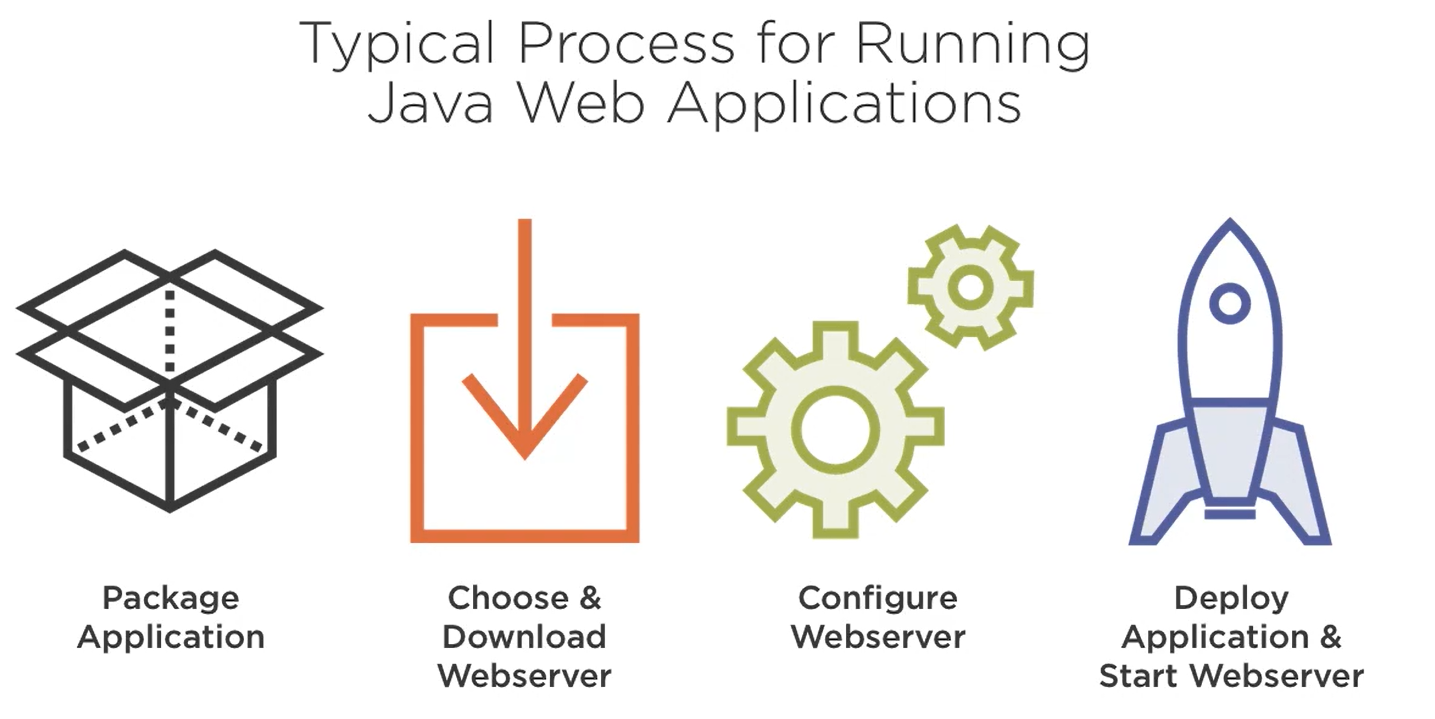
\includegraphics[width=\textwidth]{./images/chapter1/before_spring_boot.png} 

Spring came into being in 2003 as a response to the complexity of the early J2EE specifications. While some consider Java EE and its modern-day successor Jakarta EE to be in competition with Spring, they are in fact complementary. The Spring programming model does not embrace the Jakarta EE platform specification; rather, it integrates with carefully selected individual specifications from the traditional EE umbrella. Spring started as a lightweight alternative to Java Enterprise Edition. Rather than develop components as heavyweight Enterprise
JavaBeans (EJBs), Spring offered a simpler approach to enterprise Java development, utilizing dependency injection and aspect-oriented programming to achieve the capabilities of EJB with plain old Java objects (POJOs).
But while Spring was lightweight in terms of component code, it was heavyweight in terms of configuration. Initially, Spring was configured with XML (and lots of it).
It provides everything you need to create Java enterprise applications. Spring offers the flexibility to create many kinds of architectures depending on an application’s needs. As of Spring Framework 6.0, Spring requires Java 17+.

De lente ontstond in 2003 als reactie op de complexiteit van de vroege J2EE-specificaties. Hoewel sommigen Java EE en zijn moderne opvolger Jakarta EE als concurrenten van Spring beschouwen, zijn ze in feite complementair. Het Spring-programmeringsmodel omarmt niet de Jakarta EE platformspecificatie; in plaats daarvan integreert het met nauwkeurig geselecteerde individuele specificaties uit het traditionele EE-landschap. Spring begon als een lichtgewicht alternatief voor Java Enterprise Edition. In plaats van componenten te ontwikkelen als zware Enterprise JavaBeans (EJB's), bood Spring een eenvoudigere benadering voor enterprise Java-ontwikkeling, waarbij gebruik werd gemaakt van afhankelijkheidsinjectie en aspectgeoriënteerde programmering om de mogelijkheden van EJB te bereiken met gewone Java-objecten (POJO's).
Maar hoewel Spring lichtgewicht was qua componentcode, was het zwaar qua configuratie. In het begin werd Spring geconfigureerd met XML (en veel ervan).
Het biedt alles wat je nodig hebt om Java enterprise-applicaties te maken. Spring biedt de flexibiliteit om verschillende soorten architecturen te creëren, afhankelijk van de behoeften van een applicatie. Vanaf Spring Framework 6.0 vereist Spring Java 17+.

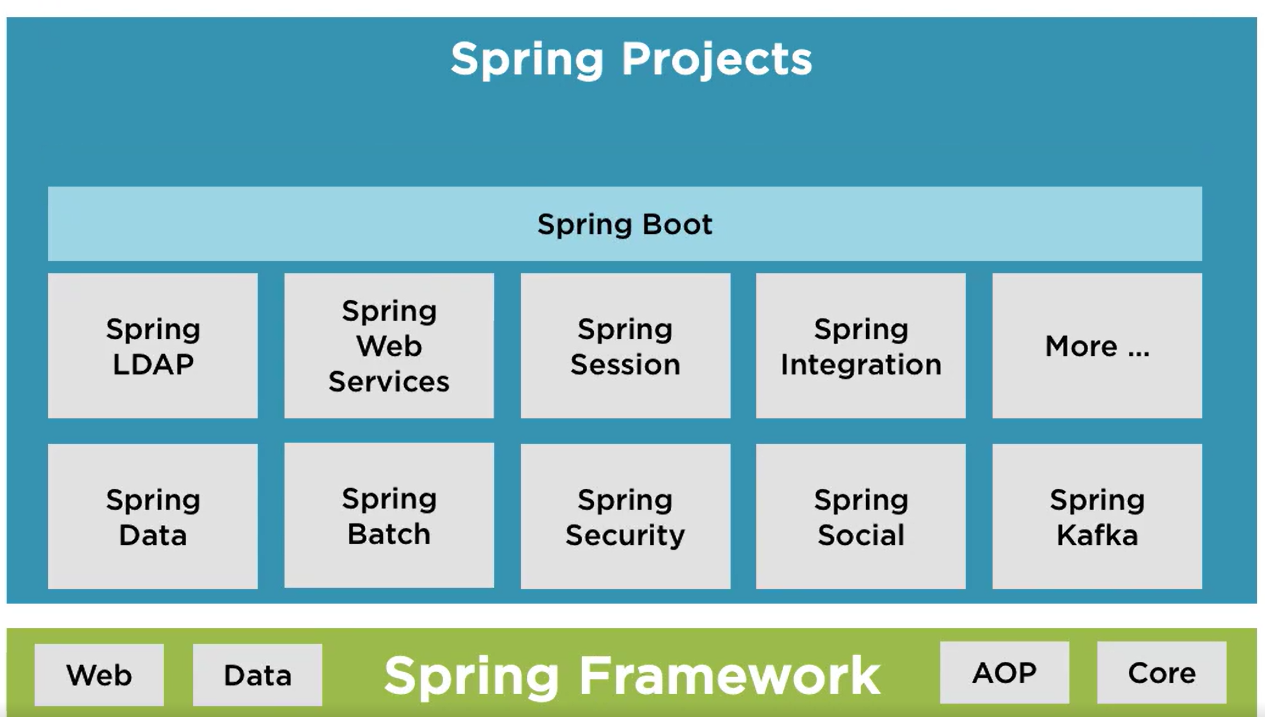
\includegraphics[width=\textwidth]{./images/chapter1/spring_framework.png} 

Spring Boot is a project that is built on the top of the Spring Framework. It provides an easier and faster way to set up, configure, and run java applications.

    
\section{What is Spring Boot?}
 
Spring Boot is an open-source Java framework to create production-ready,  standalone Spring applications. It's a robust, widely used framework. The creation of this framework was facilitated by the desire to simplify the development of applications on the popular Java EE technology stack from Oracle, which was very complex and difficult to use at the time. With very little configuration, you can create easily your first Spring Boot application.

Let's look at some advantages of Spring Boot for developers 
\begin{itemize}
\item speed up the process of creating and deploying application
\item create standalone applications with less or almost no configuration overhead
\item easy to learn framework
\item increase productivity of developers
\end{itemize}

\section{Bootstrapping a simple application}

\subsection{Using Spring Initializr}
Spring Initializr is a web application that can generate a Spring Boot project.
The url for this web application is \url{https://start.spring.io/}. You can select the necessary configuration, including the build tool, language, version of the Spring Boot framework, and any dependencies for your project. IntelliJ IDEA Ultimate provides the Spring Initializr project wizard that integrates with the Spring Initializr API to generate and import your project directly from the IDE.

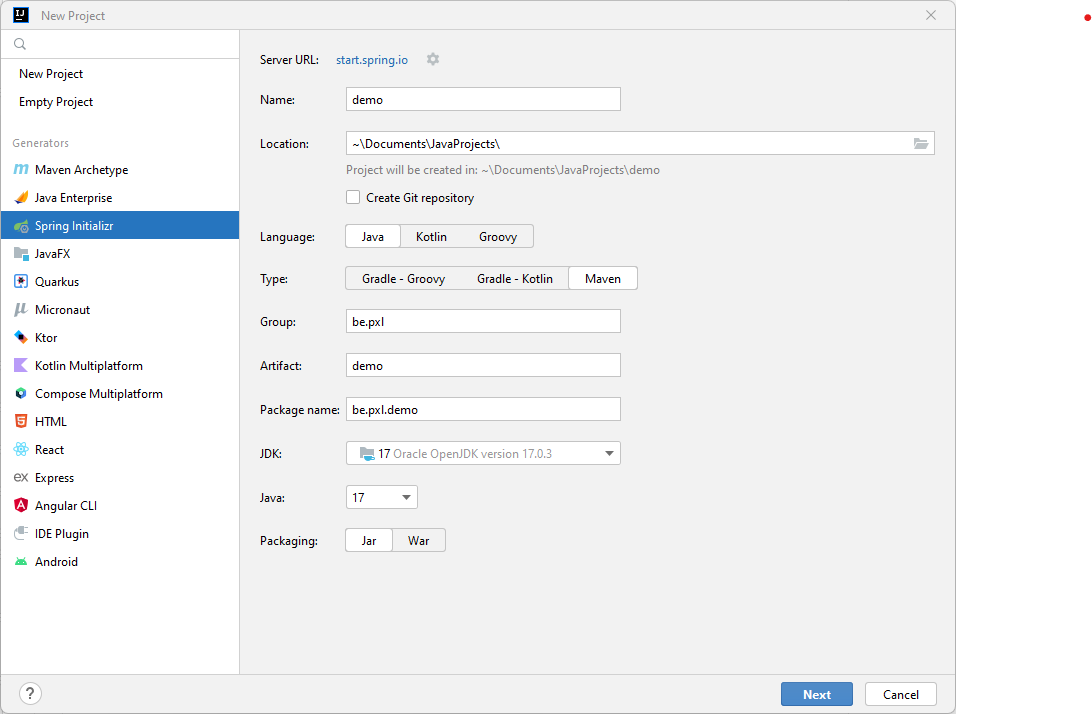
\includegraphics[width=\textwidth]{./images/chapter1/spring_initializer_intellij.png}

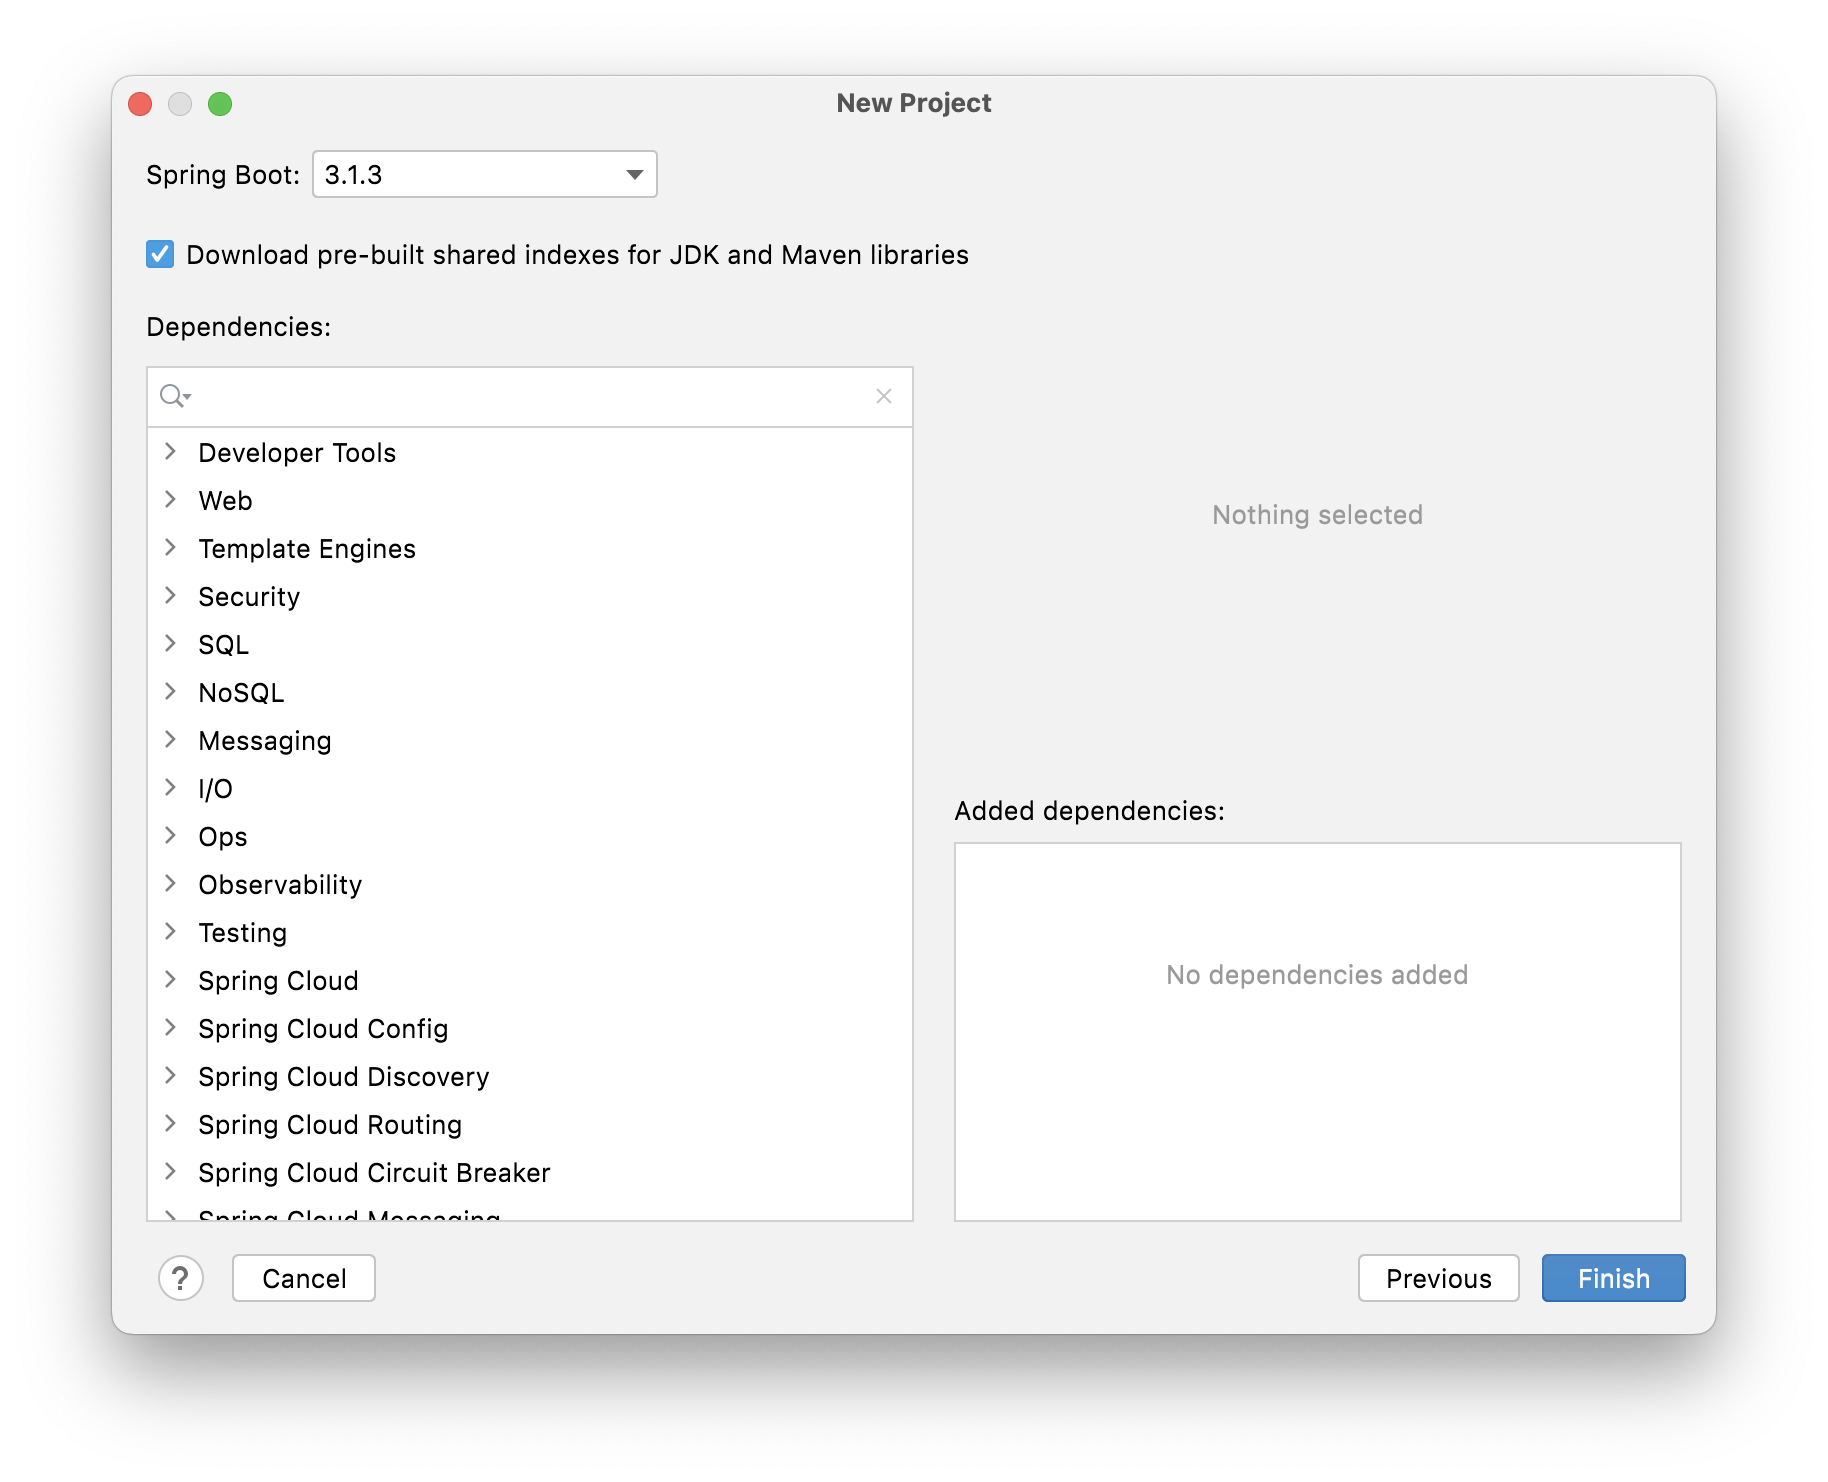
\includegraphics[width=\textwidth]{./images/chapter1/new_project.png}

We select Spring Web dependency. Spring Web uses Spring MVC. It is used for building RESTful Web Services. Spring MVC provides the annotation @RestController for classes that implement the REST endpoints.
To run a RESTful Web Service you need a web container. Spring Boot will automatically add an embedded Tomcat web container to your project. If you prefer another web container, you can update Spring Boot's configuration.
Finally Jackson is a popular third-party library for converting Java-objects to JSON and vice versa.

\begin{oefening}
Create the demo project. You can use the wizard in IntelliJ IDEA Ultimate or \url{https://start.spring.io/}.
\end{oefening}

\section{Running the demo project}

The starting point of a Spring Boot application is the class with the main-method and annotated with @SpringBootApplication.  This class can be found in the folder /src/main/java.  Spring Boot offers a lot of annotations to reduce the workload of developers.   

\begin{lstlisting}[frame=single]
package be.pxl.demo;

import org.springframework.boot.SpringApplication;
import org.springframework.boot.autoconfigure.SpringBootApplication;

@SpringBootApplication
public class DemoApplication {

    public static void main(String[] args) {
        SpringApplication.run(DemoApplication.class, args);
    }

}
\end{lstlisting}

By running the main-class you start your Spring Boot application. 

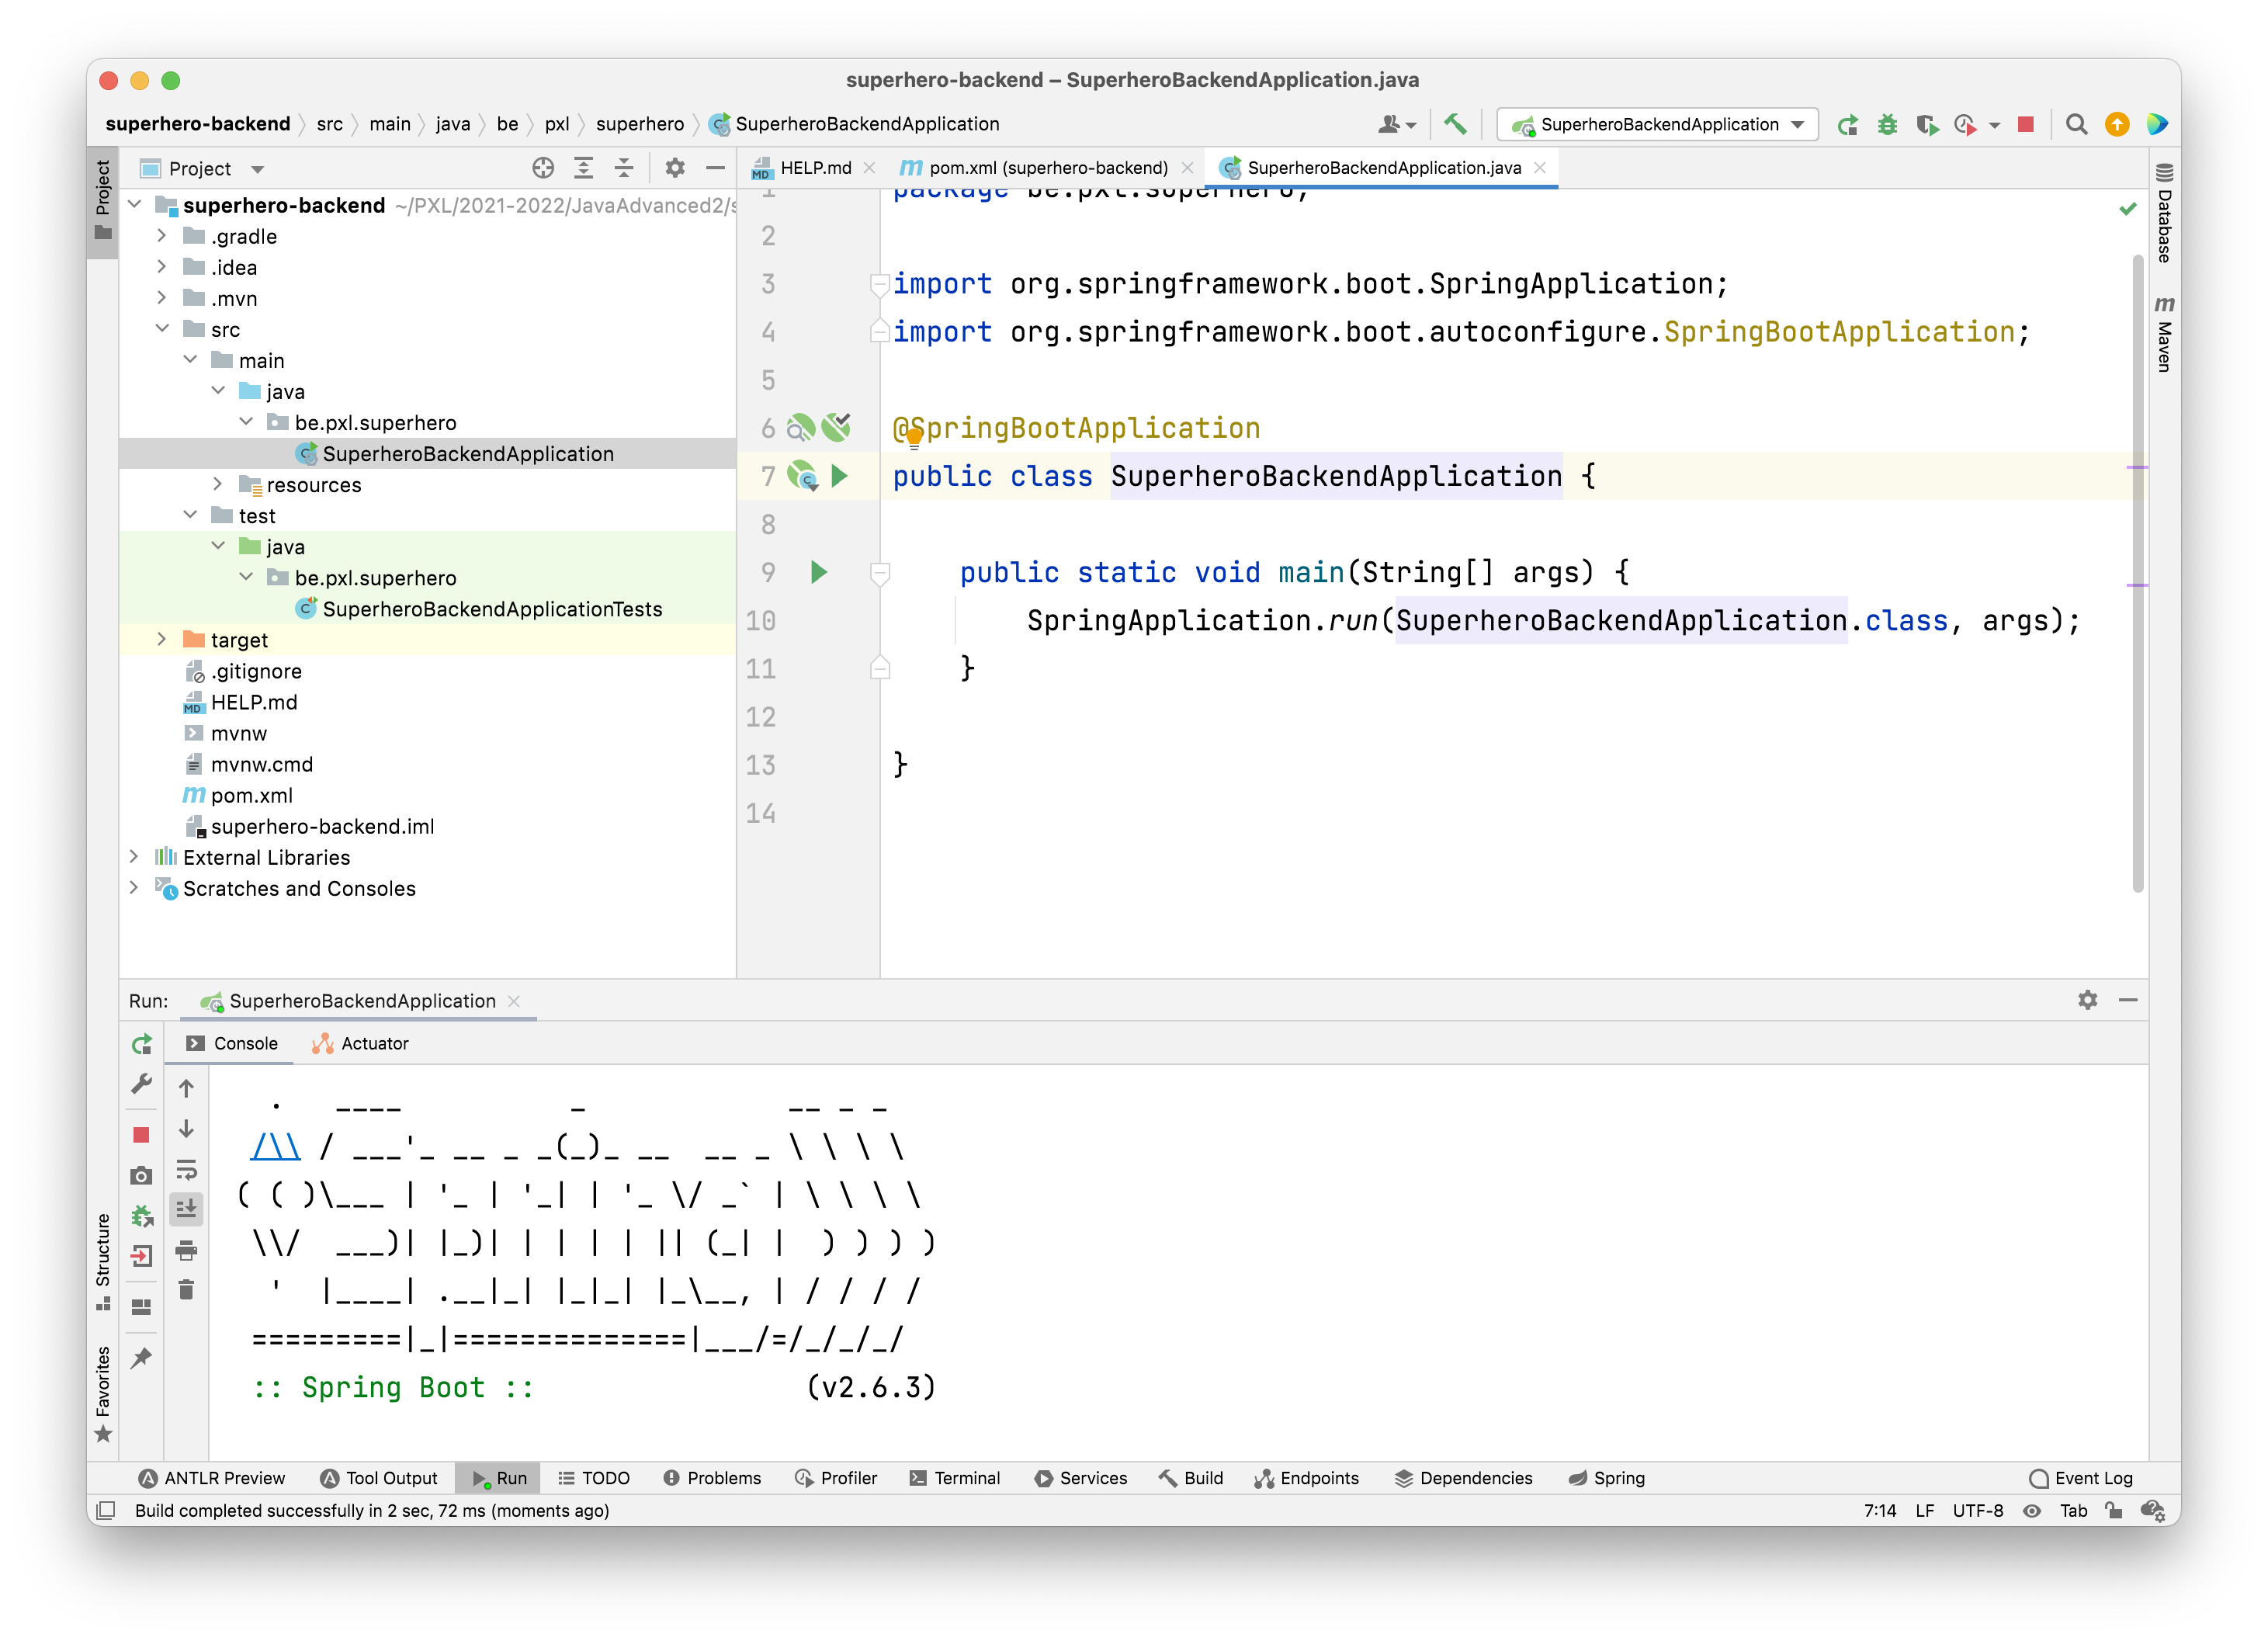
\includegraphics[width=\textwidth]{./images/chapter2/first-run.png}

Currently our Spring Boot application only shows a whitelabel error page. This error page is available when you perform a GET for URL \url{http://localhost:8080}.

\frame{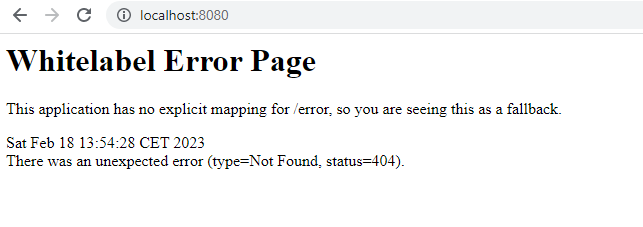
\includegraphics[width=\textwidth]{./images/chapter2/whitelabel_error_page.png}} 

Port 8080 is the default port. If this port is not available you will see an error message in Spring Boot's logging.

\begin{lstlisting}[frame=single]
***************************
APPLICATION FAILED TO START
***************************

Description:

Web server failed to start. Port 8080 was already in use.
\end{lstlisting}

The port number can be changed in the file application.properties. You have to add the property server.port here with the desired port number.

\begin{lstlisting}[frame=single]
server.port=8081
\end{lstlisting}

\subsection{Component}


\begin{lstlisting}
@Component
public class DependencyInjectionWithSpring implements CommandLineRunner {
   
   @Override    
   public void run(String... args) throws Exception {
	   System.out.println("Welcome to Java Advanced");
   }
}
\end{lstlisting}

De Spring Boot de CommandLineRunner interface voorziet de mogelijkheid om een stukje code uit te voeren zodra de Spring Boot applicatie ge\"initialiseerd is. 

Zodra je de CommandLineRunner interface implementeert in een klasse kan je de run-methode overschrijven. In de run-methode plaats je de code die uitgevoerd moet worden
als de applicatie opstart.  Zodra de Spring Boot applicatie opstart worden een aantal initialisatie-fasen doorlopen.  Eerst wordt de \textbf{application context} aangemaakt en alle Spring beans worden geladen. Als de applicatie volledige is ge\"initialiseerd wordt de run-methode van de CommandLineRunner automatisch door het Spring boot framework aangeroepen.



\subsubsection{Spring beans}

Spring Beans zijn componenten die volledig worden beheerd door het Spring Boot framework. Je hoeft zelf geen instanties van deze klassen te maken, Spring Boot genereert de objecten automatisch.  Daarnaast beheert Spring Boot ook de objecten. Wanneer een klasse gebruik wil maken van de functionaliteiten van een dergelijke Spring Bean, zal Spring Boot ervoor zorgen dat de instantie van de Spring Bean beschikbaar is voor de betreffende klasse.

\subsubsection{Application context}

De Application context is een belangrijk onderdeel van elke Spring Boot applicatie.
Hierin wordt namelijk bijgehouden welke infals een slimme doos waarin alle informatie en instellingen voor je Spring Boot-toepassing worden bewaard. Deze doos zorgt ervoor dat alle onderdelen van je applicatie met elkaar kunnen praten en weten waar ze moeten zoeken voor dingen zoals configuratie, gegevensbronnen en andere beans (componenten). Het maakt je Spring Boot-applicatie georganiseerd en helpt deze soepel te werken door alles op één plek te houden. Je kunt de application context beschouwen als het brein van je Spring Boot-applicatie dat alles coördineert en beschikbaar maakt voor de verschillende onderdelen van je programma.


Iets meer info tonen:

spring.application.name=My Demo

package be.pxl.demo.beans;

import org.springframework.boot.CommandLineRunner;
import org.springframework.context.ApplicationContext;
import org.springframework.stereotype.Component;

import java.time.LocalDateTime;
import java.time.ZoneId;
import java.time.ZoneOffset;

@Component
public class DependencyInjectionWithSpring implements CommandLineRunner {
	private final ApplicationContext applicationContext;

	public DependencyInjectionWithSpring(ApplicationContext applicationContext) {
		this.applicationContext = applicationContext;
	}

	@Override
   public void run(String... args) throws Exception {
	   System.out.println("Welcome to Java Advanced");
		System.out.println(applicationContext.getApplicationName());
		System.out.println(applicationContext.getDisplayName());
		System.out.println(applicationContext.getId());
		LocalDateTime dateTime = convertStartupDateToLocalDateTime(applicationContext.getStartupDate());
		System.out.println(dateTime);
		System.out.println(LocalDateTime.now());
   }


   private LocalDateTime convertStartupDateToLocalDateTime(long startupDate) {
	   // Get the system's default timezone
	   ZoneId systemZoneId = ZoneId.systemDefault();
	   // Get the ZoneOffset for the system's default timezone
	   ZoneOffset systemZoneOffset = systemZoneId.getRules().getOffset(LocalDateTime.now());
		return LocalDateTime.ofEpochSecond(applicationContext.getStartupDate() / 1000, 0, systemZoneOffset);

   }
}



Spring Boot Application Context:
When your Spring Boot application starts, it goes through various phases of initialization. After the application context is prepared and all beans are loaded, any classes implementing CommandLineRunner are executed.

\subsection{The Maven pom file}

POM stands for \'Project Object Model\'. It is an XML representation of a Maven project held in a file named pom.xml. This file can be found in your project directory. The POM contains all necessary information about a project, as well as configurations of plugins to be used during the build process. We will cover Maven in chapter 3.

\begin{lstlisting}[frame=single]
<?xml version="1.0" encoding="UTF-8"?>
<project xmlns="http://maven.apache.org/POM/4.0.0" xmlns:xsi="http://www.w3.org/2001/XMLSchema-instance"
         xsi:schemaLocation="http://maven.apache.org/POM/4.0.0 https://maven.apache.org/xsd/maven-4.0.0.xsd">
    <modelVersion>4.0.0</modelVersion>
    <parent>
        <groupId>org.springframework.boot</groupId>
        <artifactId>spring-boot-starter-parent</artifactId>
        <version>3.0.2</version>
        <relativePath/> <!-- lookup parent from repository -->
    </parent>
    <groupId>be.pxl</groupId>
    <artifactId>demo</artifactId>
    <version>0.0.1-SNAPSHOT</version>
    <name>demo</name>
    <description>demo</description>
    <properties>
        <java.version>17</java.version>
    </properties>
    <dependencies>
        <dependency>
            <groupId>org.springframework.boot</groupId>
            <artifactId>spring-boot-starter-web</artifactId>
        </dependency>

        <dependency>
            <groupId>org.springframework.boot</groupId>
            <artifactId>spring-boot-starter-test</artifactId>
            <scope>test</scope>
        </dependency>
    </dependencies>

    <build>
        <plugins>
            <plugin>
                <groupId>org.springframework.boot</groupId>
                <artifactId>spring-boot-maven-plugin</artifactId>
            </plugin>
        </plugins>
    </build>
</project>
\end{lstlisting}

spring-boot-starter-parent is a starter project that provides the default configuration for spring-based applications. Here you choose the version of Spring Boot.

For large projects, managing the dependencies is not always easy. Spring Boot solves this problem by grouping certain dependencies together. These groups of dependencies are called starters. All Spring Boot starters are named following the same naming pattern. The all start with spring-boot-starter-*, where * indicates the purpose and functionality provided by the starter.

spring-boot-starter-web adds all the libraries we need to develop web components. An embedded server will be provided in the Spring Boot project. Therefore the environment where the Spring Boot project is executed does not need to have a pre-installed server. The default embedded server for Spring Boot is Tomcat. The Spring MVC framework which provides all classes for developing RESTful web services is also part of spring-boot-starter-web.

spring-boot-starter-test (with scope test) is the starter for testing Spring Boot applications with libraries including JUnit Jupiter, Hamcrest and Mockito.

Inversion of Control (IoC) is \'e\'en van de basisprincipes van het Spring framework.
Bij Inversion of Control is het aanmaken en beheren van objecten niet langer de verantwoordelijkheid van de objecten zelf, maar is er een aparte 

So, Inversion of Control is about shifting the responsibility of managing object interactions from your code to a higher-level component (the framework or container). This makes your code more modular and flexible, as you rely on the framework to provide and coordinate the necessary components, 

To explain this in layman's terms, suppose you drive a car to your work place. This means you control the car. The IoC principle suggests to invert the control, meaning that instead of driving the car yourself, you hire a cab, where another person will drive the car.

What is a Bean in Spring Boot? A Bean is an object that is managed by the Spring framework. It is created, managed, and managed by the Spring container. Beans can be used to encapsulate and provide services, utilities, and functionalities to other components in an application.

In Spring, the objects that form the backbone of your application and that are managed by the Spring IoC container are called beans. A bean is an object that is instantiated, assembled, and otherwise managed by a Spring IoC container. Otherwise, a bean is simply one of many objects in your application.

TODO add image





IOC en dependency injection 


@Component
public class DependencyInjectionWithSpring implements CommandLineRunner {
   
   @Autowired
   private WeatherService weatherService;
   
   @Override    
   public void run(String... args) throws Exception {
	   weatherService.printWeather();
   }
}

WeatherService.java

import org.springframework.stereotype.Component;

@Component
public class WeatherService {
   public void printWeather() {
      System.out.println("The weather is sunny with a 20% chance of rain");
   }
}


Exercise

Create the class 





\subsection{@SpringBootApplication}

Java annotations are a mechanism for adding metadata information to our source code. An annotation processor processes these annotations at compile time or runtime to provide functionality such as code generation, error checking, etc.

@SpringBootApplication annotation is used to enable following three features:
\begin{itemize}
\item @EnableAutoConfiguration: enable Spring Boot’s auto-configuration mechanism
\item @ComponentScan: enable @Component scan on the package where the application is located
\item @Configuration: allow to register extra beans in the context or import additional configuration classes
\end{itemize}


\subsection{Auto-configuration}

Spring Boot auto-configuration attempts to automatically configure your Spring application based on the dependencies that you have added.
To gain some insight in this auto-configuration let's add a line in the application.properties file. This file can be found in the directory /src/main/resources. 

\begin{lstlisting}
logging.level.org.springframework=debug
\end{lstlisting}

logging.level.org.springframework is a application properties. A list of all available application properties can be found at \url{https://docs.spring.io/spring-boot/docs/current/reference/html/application-properties.html}.

\begin{oefening}
Add the line above to the application.properties file and restart the Spring Boot application.
\end{oefening}

In the console you will find all the auto-configuration Spring Boot is doing.

\chapter{REST}

\fcolorbox{black}[HTML]{E9F0E9}{\parbox{\textwidth}{%
\noindent \textbf{Learning goals}\\
De junior-collega
\begin{enumerate}[nolistsep]
\item kan beschrijven wat een RESTful web applicatie is
\item kan een POST, GET, PUT en DELETE-verzoek afhandelen in Spring Boot
\item kan beschrijven wat spring-boot-starter-web is
\item 
\end{enumerate}}}

\section{HTTP-verzoekmethoden}

Spring Boot is een goede keuze als je een REST API (of voluit een RESTful web API) wilt ontwikkelen in Java.

REST (Representational State Transfer) is een gestandaardiseerde manier om communicatie tussen verschillende softwaretoepassingen over het internet mogelijk te maken. 
In een RESTful web applicatie wordt de functionaliteit van de applicatie beschikbaar gesteld als resources, die kunnen worden geïdentificeerd door URI's (Uniform Resource Identifiers).  Gebruikers en andere applicaties kunnen met deze resources communiceren via standaard HTTP-verzoekmethoden (HTTP-request, HTTP-method of HTTP-verb). In essentie is HTTP het transportprotocol dat wordt gebruikt om gegevens over te dragen,  terwijl REST de verzameling van ontwerpprincipes is die bepalen hoe die gegevens moeten worden georganiseerd en benaderd.

\begin{itemize}
\item \textbf{GET}: Het GET-verzoek wordt gebruikt om gegevens op te halen van een specifieke resource. 

Voorbeeld URI: GET /api/products/123

Dit verzoek haalt informatie op over het product met ID 123.

\item \textbf{POST}: Het POST-verzoek wordt gebruikt om nieuwe gegevens naar een resource te verzenden. Het wordt vaak gebruikt voor het maken van nieuwe resources of het toevoegen van gegevens aan een bestaande resource.

Voorbeeld URI: POST /api/products

Dit verzoek voegt een nieuw product toe aan de lijst van producten.

\item \textbf{PUT}: Het PUT-verzoek wordt gebruikt om gegevens bij te werken voor een specifieke resource of om een nieuwe resource te maken als deze niet bestaat. Het is idempotent, wat betekent dat meerdere PUT-verzoeken hetzelfde resultaat opleveren.

Voorbeeld URI: PUT /api/products/123

Dit verzoek bijwerken de informatie van het product met ID 123.

\item \textbf{DELETE}: Het DELETE-verzoek wordt gebruikt om een resource te verwijderen of te deactiveren.

Voorbeeld URI: DELETE /api/products/123

Dit verzoek verwijdert het product met ID 123 uit de lijst van producten.
\end{itemize}

\section{Spring Boot Starter Web}

Spring Boot Starter Web is de verzameling van alle bibliotheken (third party libraries) die we nodig hebben om RESTful web applicaties te bouwen.  De verzameling bestaat ondermeer uit Spring MVC,  REST,  jackson en Tomcat. 
Apache Tomcat is een populaire open source web server voor Java toepassingen.  Als je de dependency spring-boot-start-web toevoegt, start de Tomcat web server op zodra je de Spring boot applicatie opstart.  We spreken van de "embedded web server" in Spring boot.  Je kan er ook voor kiezen om  \'e\'en van de alternatieve web servers te gebruiken zoals jetty of undertow. 
Jackson is een populaire library om Java-objecten naar JSON te converteren en vice versa.

\begin{lstlisting}
<dependency>
		<groupId>org.springframework.boot</groupId>
		<artifactId>spring-boot-starter-web</artifactId>
</dependency>
\end{lstlisting}
		
Je voegt de dependency toe in het bestand pom.xml.
		
Start nu de Spring Boot applicatie opnieuw op.

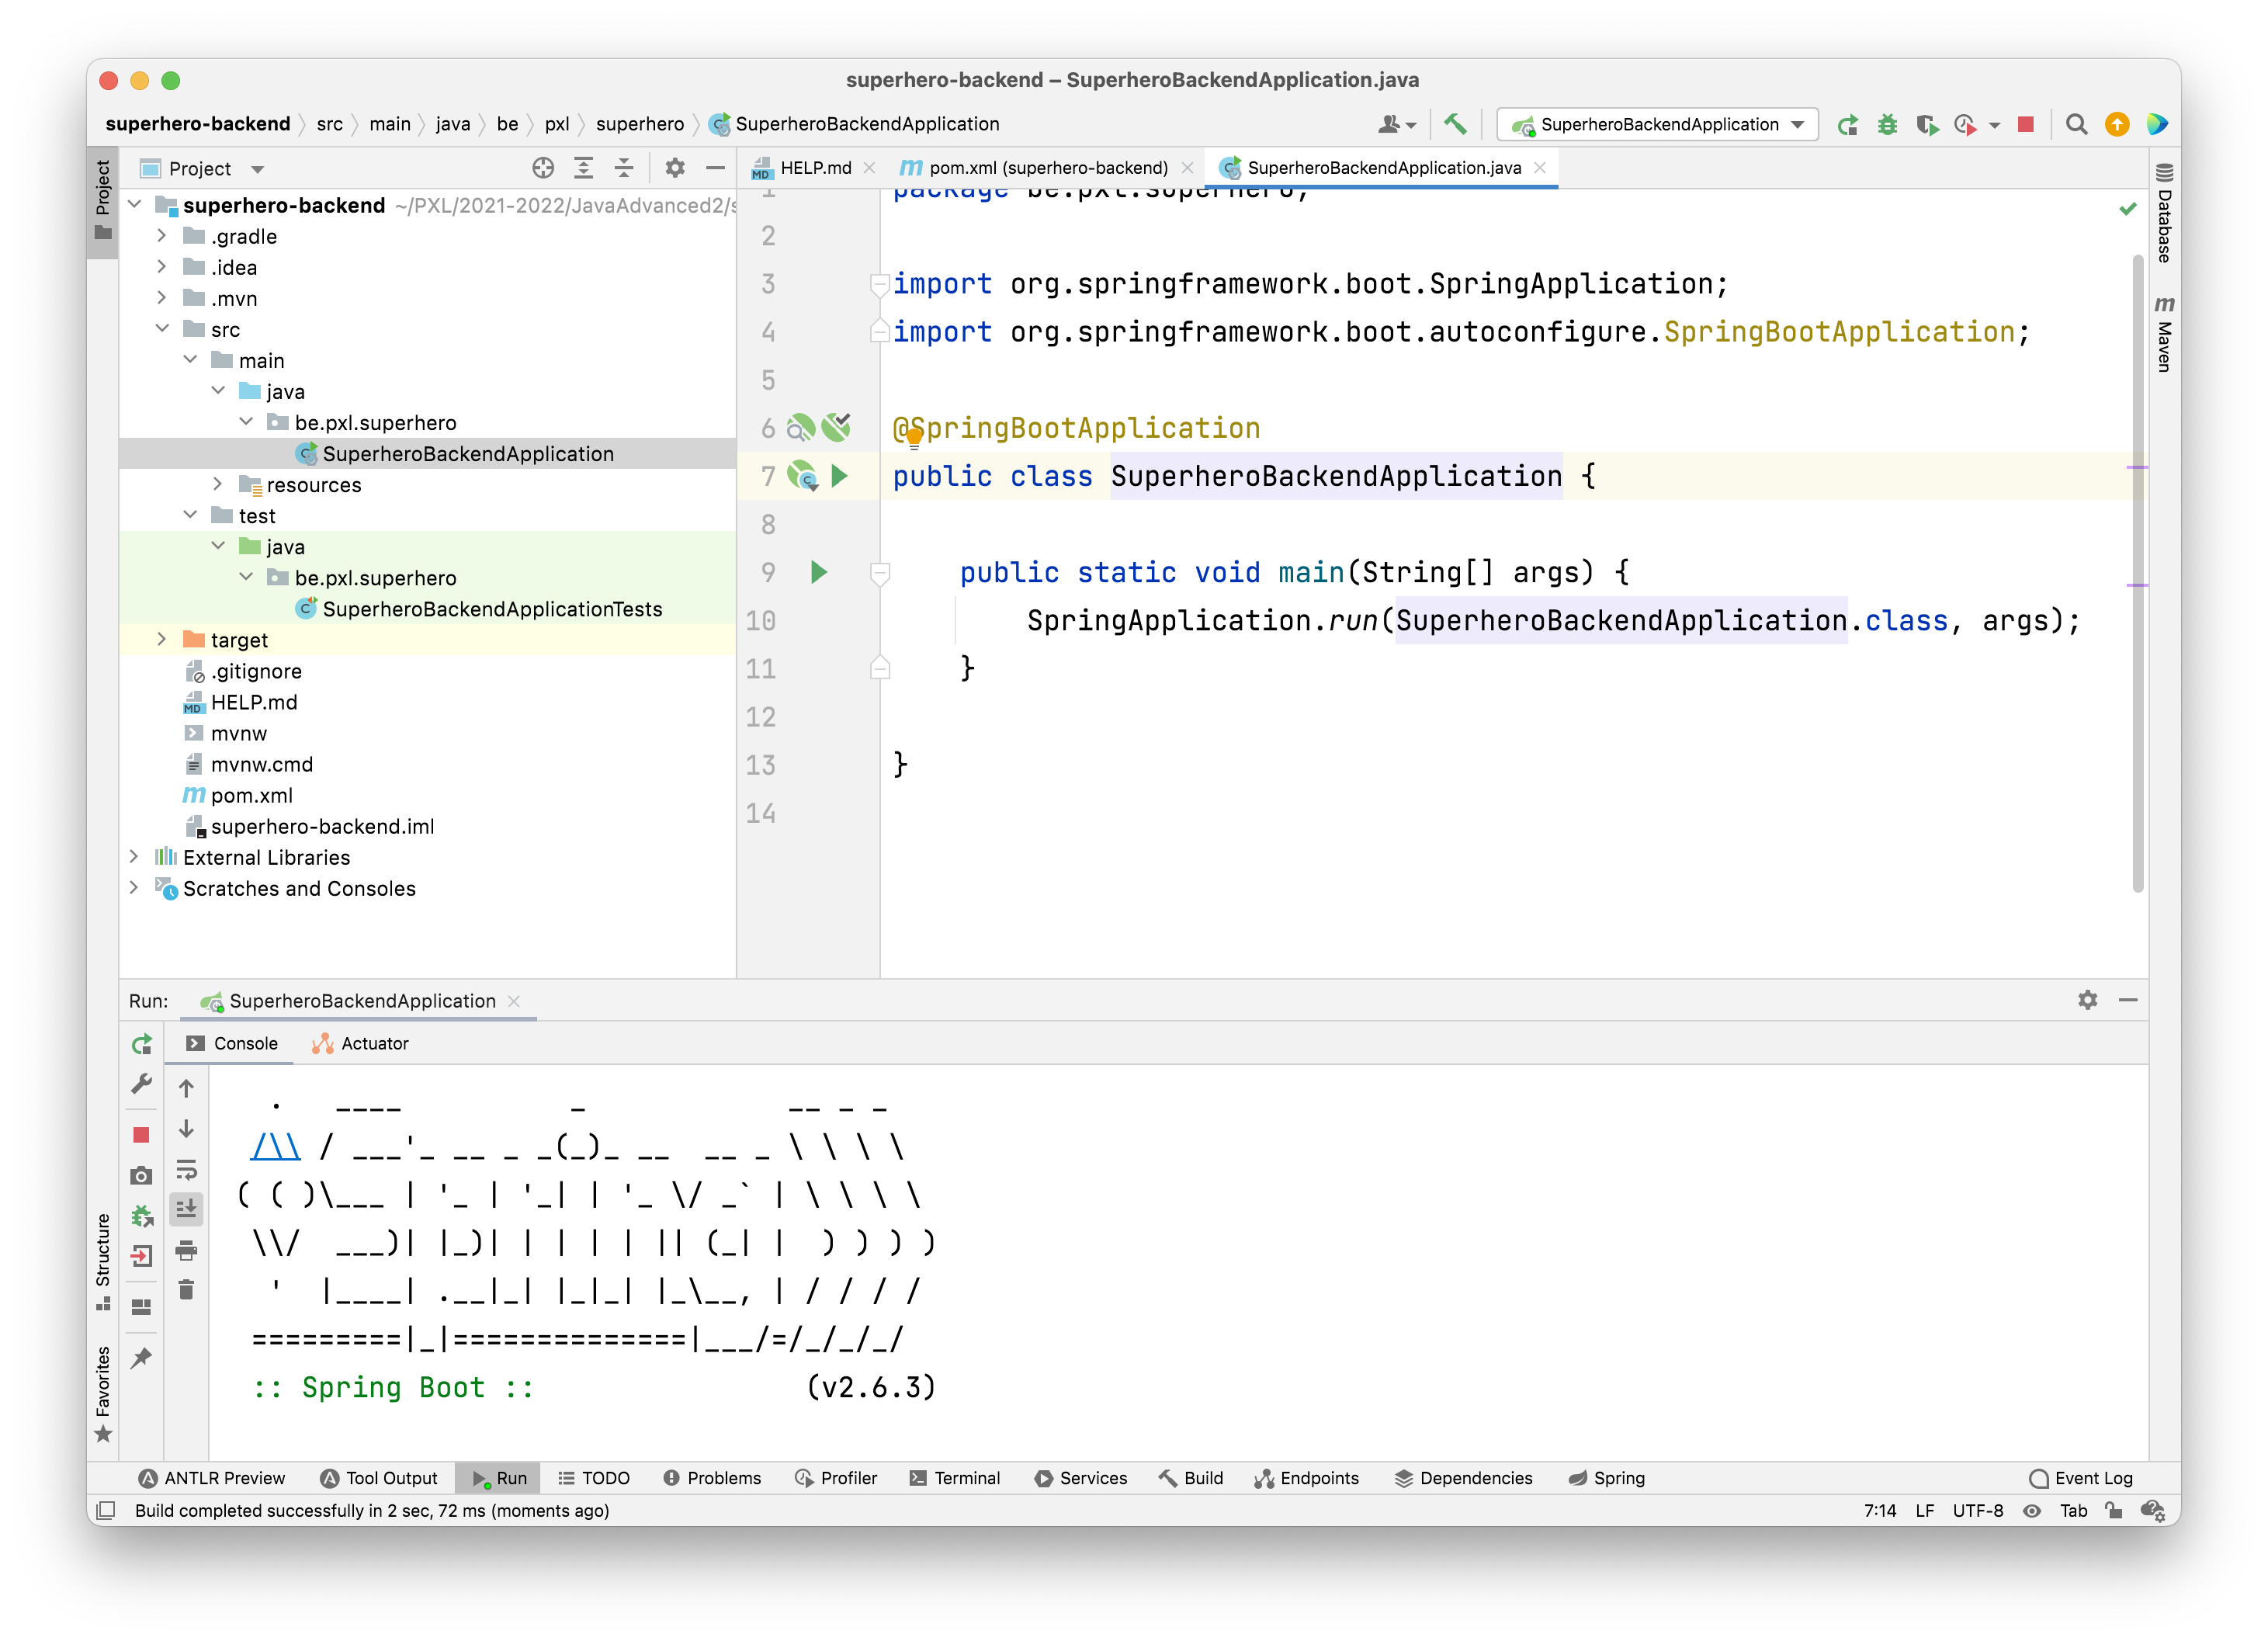
\includegraphics[width=\textwidth]{./images/chapter2/first-run.png}

Momenteel kan de Spring Boot applicatie enkel een whitelabel error pagina tonen.  De error pagina krijg je te zien als je een GET-request uitvoert voor URL \url{http://localhost:8080}.

\frame{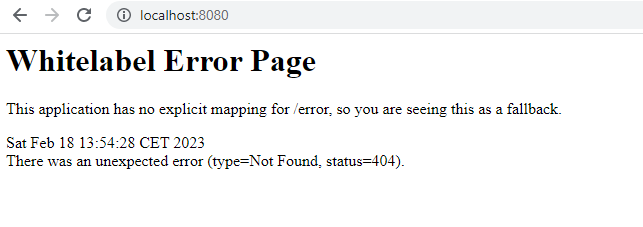
\includegraphics[width=\textwidth]{./images/chapter2/whitelabel_error_page.png}} 

Poort 8080 is de default poort van de Tomcat webserver.  Als deze poort al gebruikt wordt door een ander programma, krijg je de volgende foutmelding te zien.

\begin{lstlisting}[frame=single]
***************************
APPLICATION FAILED TO START
***************************

Description:

Web server failed to start. Port 8080 was already in use.
\end{lstlisting}

De poortnummer kan aangepast worden in het bestand application.properties.  Je gebruikt de eigenschap \textbf{server.port} om de gewenste poortnummer te kiezen.

\begin{lstlisting}[frame=single]
server.port=8081
\end{lstlisting}

\section{De RestController}

Spring boot heeft een annotatie voorzien voor de Spring bean die verantwoordelijk is voor het afhandelen van HTTP requests nl. @RestController. Spring boot heeft ook een annotatie @Controller, maar de @RestController zorgt ervoor dat het respons op het HTTP-request automatisch wordt omgezet (geserialiseerd) naar JSON of XML en wordt teruggestuurd naar de client.


\begin{lstlisting}[frame=single]
package be.pxl.demo.api;

import jakarta.annotation.PostConstruct;
import org.springframework.web.bind.annotation.GetMapping;
import org.springframework.web.bind.annotation.RestController;

import java.util.ArrayList;
import java.util.List;
import java.util.Random;

@RestController
@RequestMapping("/greetings")
public class GreetingController {

    private final List<String> messages = new ArrayList<>();
    private static final Random RANDOM = new Random();

    @PostConstruct
    public void init() {
        messages.add("Peek-a-boo!");
        messages.add("Howdy-doody!");
        messages.add("My name's Ralph, and I'm a bad guy.");
        messages.add("I come in peace!");
        messages.add("Put that cookie down!");

    }

    @GetMapping("/hello")
    public String doGreeting() {
        return messages.get(RANDOM.nextInt(messages.size()));
    }
}
\end{lstlisting}

De @RestController markeert de klasse GreetingController als een REST-controller.
De annotatie @RequestMapping("/greetings") specificeert het basispad voor alle requests die door deze controller worden afgehandeld.
@GetMapping("/hello") geeft aan dat de goGreeting-methode wordt uitgevoerd wanneer een HTTP GET-verzoek wordt gemaakt naar het pad "/greetings/hello". Het resultaat van deze methode wordt automatisch omgezet in tekst en teruggestuurd als de respons.

\begin{figure}[H]
  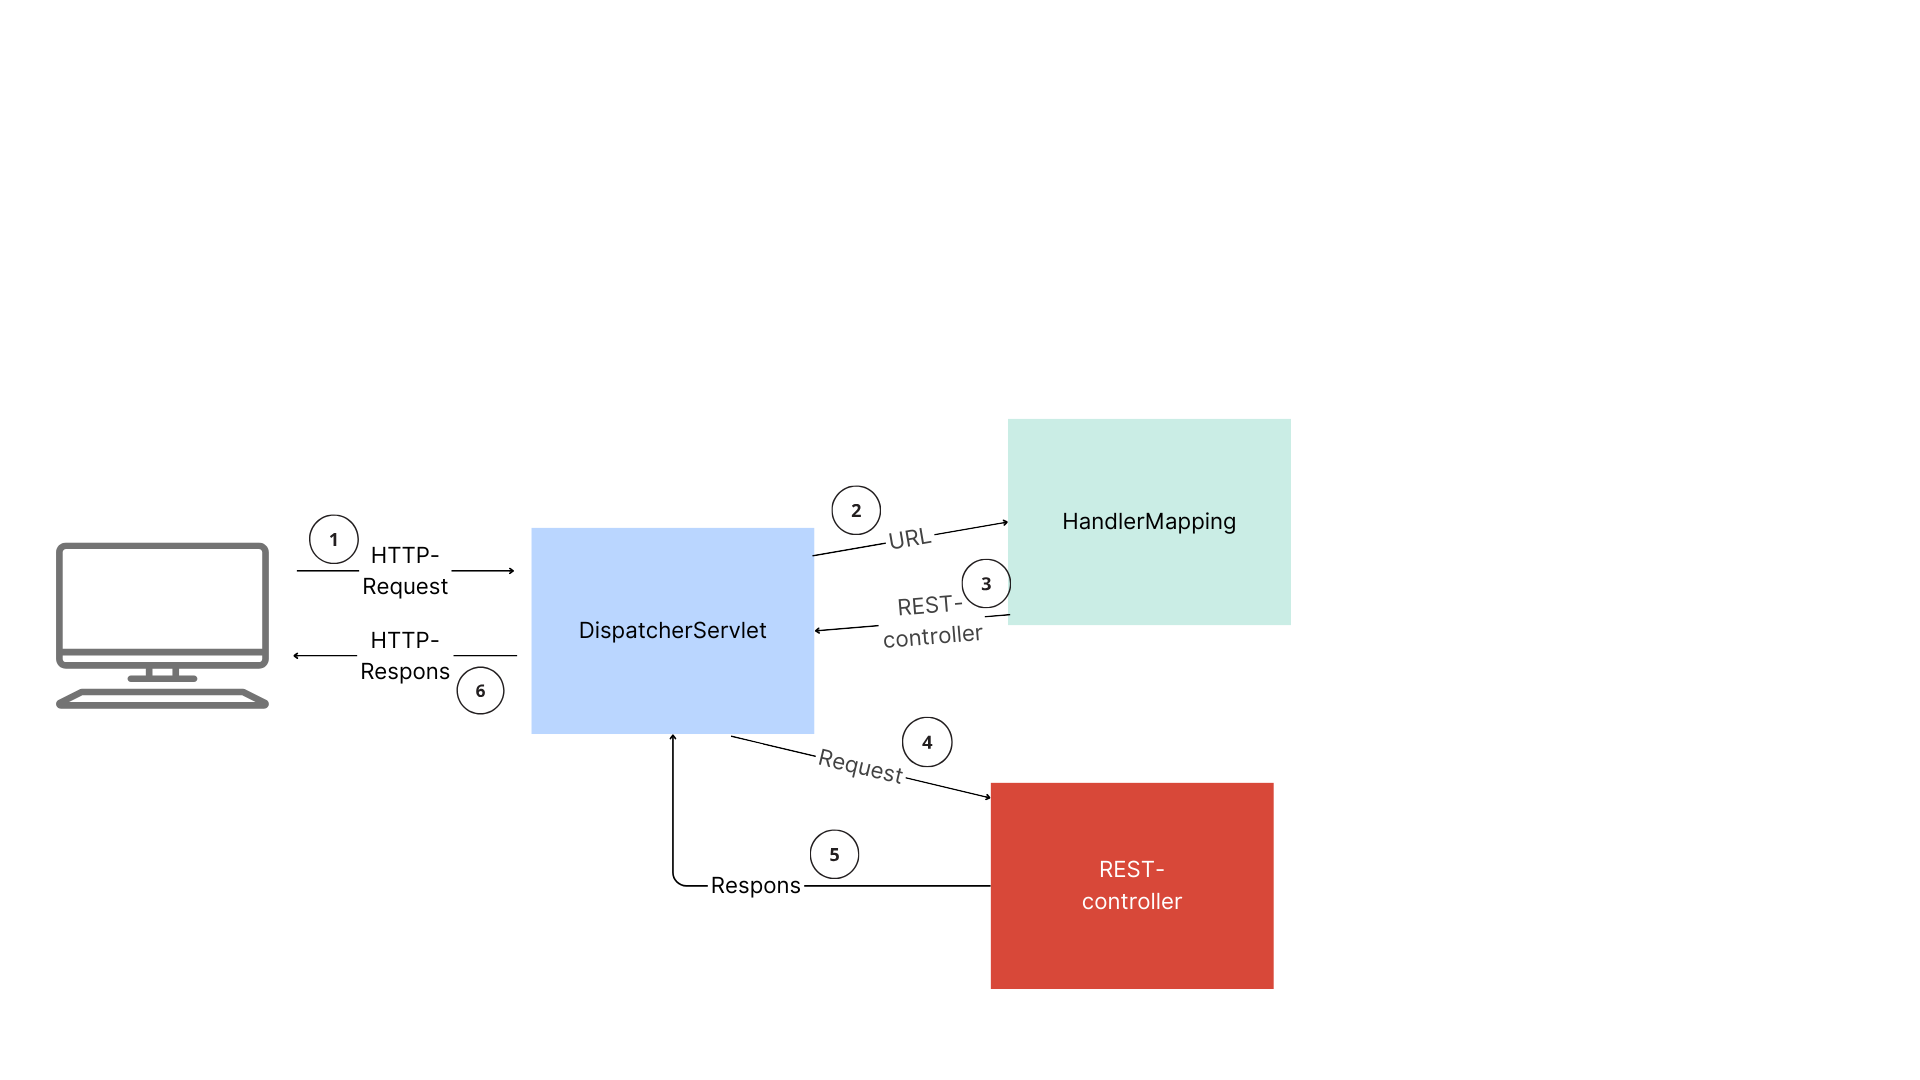
\includegraphics[width=\linewidth]{images/chapter-rest/dispatcherservlet.png}
  \caption{Een REST-verzoek afhandelen}
  \label{fig:test_passed}
\end{figure}

De component van Spring Boot die verantwoordelijk is dat een HTTP-request door de juiste REST-controller wordt afgehandeld is de DispatcherServlet.  De DispatcherServlet is onderdeel van Spring MVC.  De DispatcherServlet bepaalt welke controller een HTTP-request moet afhandelen,  hij geeft het request door aan de juiste controller en  verwerkt het respons van de controller om een HTTP-respons terug te sturen naar de client.

Om te achterhalen welke REST-controller verantwoordelijk is om een HTTP-request af te handelen raadpleegt de DispatcherServlet de HandlerMapping. De HandlerMapping is als het ware een kaart die URL's koppelt aan specifieke controllerklassen en methoden.
Op basis van de URL in het binnenkomende request bepaalt de DispatcherServlet welke controllerklasse en methode verantwoordelijk zijn voor het afhandelen van het request.


\begin{oefening}
Maak het package \textit{be.pxl.demo.api}.  Voeg de klasse \textbf{GreetingController} toe het package.  Start de Spring Boot applicatie en open de URL \url{http://localhost:8080/greetings/hello} in een browser. Voeg in de REST-controller een methode toe met de URI GET /greetings/daytime die de huidige dag en het tijdstip teruggeeft in het formaat 'Maandag 18 september 2023'.
\end{oefening}

\section{MusicPlaylist}

We gaan een nieuwe Spring Boot toepassing aanmaken waarmee we een muziek playlist beheren. 

\begin{oefening}
Maak een nieuwe Spring boot toepassing MusicPlaylist. We gebruiken Spring MVC om een RESTful web applicatie te maken.  
\end{oefening}

\subsection{Een liedje toevoegen aan een playlist}

\begin{apiRoute}{post}{/playlist/songs}{Add a new song to the playlist.}
\begin{routeRequest}{application/json}
\begin{routeRequestBody}
{
  "title": "Hello",
  "artist": "Adele",
  "duration_seconds": 293,
  "genre": "POP"
}
\end{routeRequestBody}
\end{routeRequest}
\begin{routeResponse}{application/json}
\begin{routeResponseItem}{200}{ok}
\end{routeResponseItem}
\end{routeResponse}
\end{apiRoute}


Om te beginnen hebben we de klasse Song nodig. 

\begin{lstlisting}[language=java,  frame=single]
public class Song {
    private String title;
    private String artist;
    @JsonProperty("duration_seconds")
    private int durationSeconds;
    private Genre genre;

    // Default constructor
    public Song() {
    }

    // Parameterized constructor
    public Song(String title, String artist, int durationSeconds, Genre genre) {
        this.title = title;
        this.artist = artist;
        this.durationSeconds = durationSeconds;
        this.genre = genre;
    }

    // Getter and setter methods
    public String getTitle() {
        return title;
    }

    public void setTitle(String title) {
        this.title = title;
    }

    public String getArtist() {
        return artist;
    }

    public void setArtist(String artist) {
        this.artist = artist;
    }

    public int getDurationSeconds() {
        return durationSeconds;
    }

    public void setDurationSeconds(int durationSeconds) {
        this.durationSeconds = durationSeconds;
    }

    public Genre getGenre() {
        return genre;
    }

    public void setGenre(Genre genre) {
        this.genre = genre;
    }

    @Override
    public String toString() {
        return "Song{" +
                "title='" + title + '\'' +
                ", artist='" + artist + '\'' +
                ", durationSeconds=" + durationSeconds +
                ", genre='" + genre + '\'' +
                '}';
    }
}
\end{lstlisting}


Nu gaan we de REST-controller implementeren.  We gaan hierin een methode voorzien die een POST op de URI /playlist/songs kan afhandelen.  Initieel gaan we enkel de titel in de loggegevens tonen. 

\begin{lstlisting}[language=java,  frame=single]
@RestController
@RequestMapping("/playlist/songs")
public class MusicPlaylistController {

	private static final Logger LOGGER = LoggerFactory.getLogger(MusicPlaylistController.class);

	@PostMapping
	public void addSong(@RequestBody Song song) {
		if (LOGGER.isInfoEnabled()) {
			LOGGER.info("Adding song [" + song.getTitle() + "]");
		}
	}
}
\end{lstlisting}

De liedjes die aan de playlist worden toegevoegd willen we bijhouden. Later zullen we ze wegschrijven in een databank, maar voorlopig gaan we ze bijhouden in een lijst.
Om dit mogelijk te maken gaan we een nieuwe Spring Bean toevoegen: de MusicPlaylistService.  

\begin{lstlisting}[language=java,  frame=single]
package be.pxl.demo;

import be.pxl.demo.domain.Song;
import org.springframework.stereotype.Service;

import java.util.ArrayList;
import java.util.List;

@Service
public class MusicPlaylistService {
	private final List<Song> myPlaylist = new ArrayList<>();

	public void addSong(Song song) {
		myPlaylist.add(song);
	}
}
\end{lstlisting}

De MusicPlaylistService wordt geannoteerd met @Service .
In onze Spring Boot applicaties gaan we steeds de business-logica implementeren in de service-laag.  De @Service annotatie wordt gebruikt voor de componenten (Spring Beans) in de service-laag.  Wanneer onze Spring Boot applicatie opstart wordt er exact \'e\'en instantie van de MusicPlaylistService aangemaakt in de ApplicationContext en deze instantie wordt tijdens de volledige levensduur van de toepassing gebruikt.  Dit noemen we de scope van de service en de default scope noemen we \textbf{singleton}. 
Dit betekent dat we \'e\'en enkele, gedeelde playlist hebben voor alle gebruikers.

Nu gaan we de MusicPlaylistService beschikbaar maken in de MusicPlaylistController.
We maken gebruik van \textbf{constructor injection}.  Zodra de instantie van de MusicPlaylistController door Spring Boot wordt aangemaakt, zal er eerst gezorgd worden dat de instantie MusicPlaylistService aangemaakt wordt. Deze instantie wordt dan achter de schermen meegegeven aan de constructor van de MusicPlaylistController. Zo kan ons MusicPlaylistController-object het MusicPlaylistService-object gebruiken.
Omdat er maar \'e\'en constructor is, is de annotatie @Autowired eigenlijk overbodig.

\begin{lstlisting}[language=java,  frame=single]
@RestController
@RequestMapping("/playlist/songs")
public class MusicPlaylistController {

	private static final Logger LOGGER = LoggerFactory.getLogger(MusicPlaylistController.class);
	private final MusicPlaylistService musicPlaylistService;

	@Autowired
	public MusicPlaylistController(MusicPlaylistService musicPlaylistService) {
		this.musicPlaylistService = musicPlaylistService;
	}

	@PostMapping
	public void addSong(@RequestBody Song song) {
		if (LOGGER.isInfoEnabled()) {
			LOGGER.info("Adding song [" + song.getTitle() + "]");
		}
		musicPlaylistService.addSong(song);
	}
}
\end{lstlisting}

Test nu het POST-verzoek.  Je kan Postman,  Insomnia of een andere tool gebruiken om een POST-verzoek naar de toepassing te sturen.  De toegevoegde liedjes gaan uiteraard verloren wanneer je de toepassing herstart. 

\begin{figure}[H]
  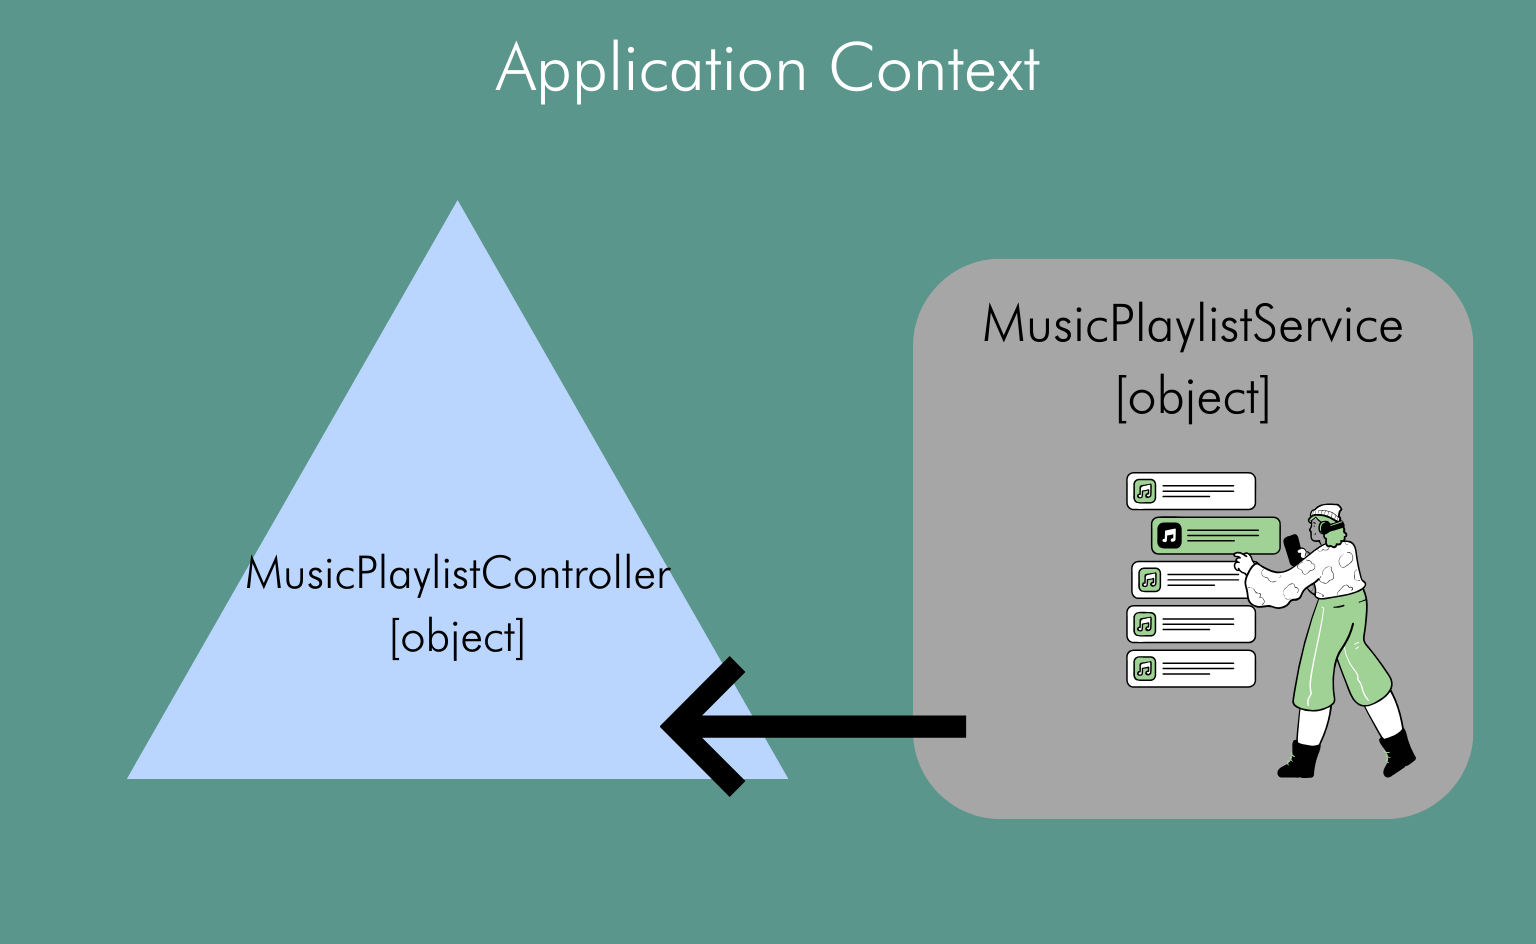
\includegraphics[width=\linewidth]{images/chapter-rest/applicationcontext_musicplaylist.png}
  \caption{Spring Beans in de Application Context}
  \label{fig:spring_beans_musicplaylist}
\end{figure}


\begin{figure}[H]
  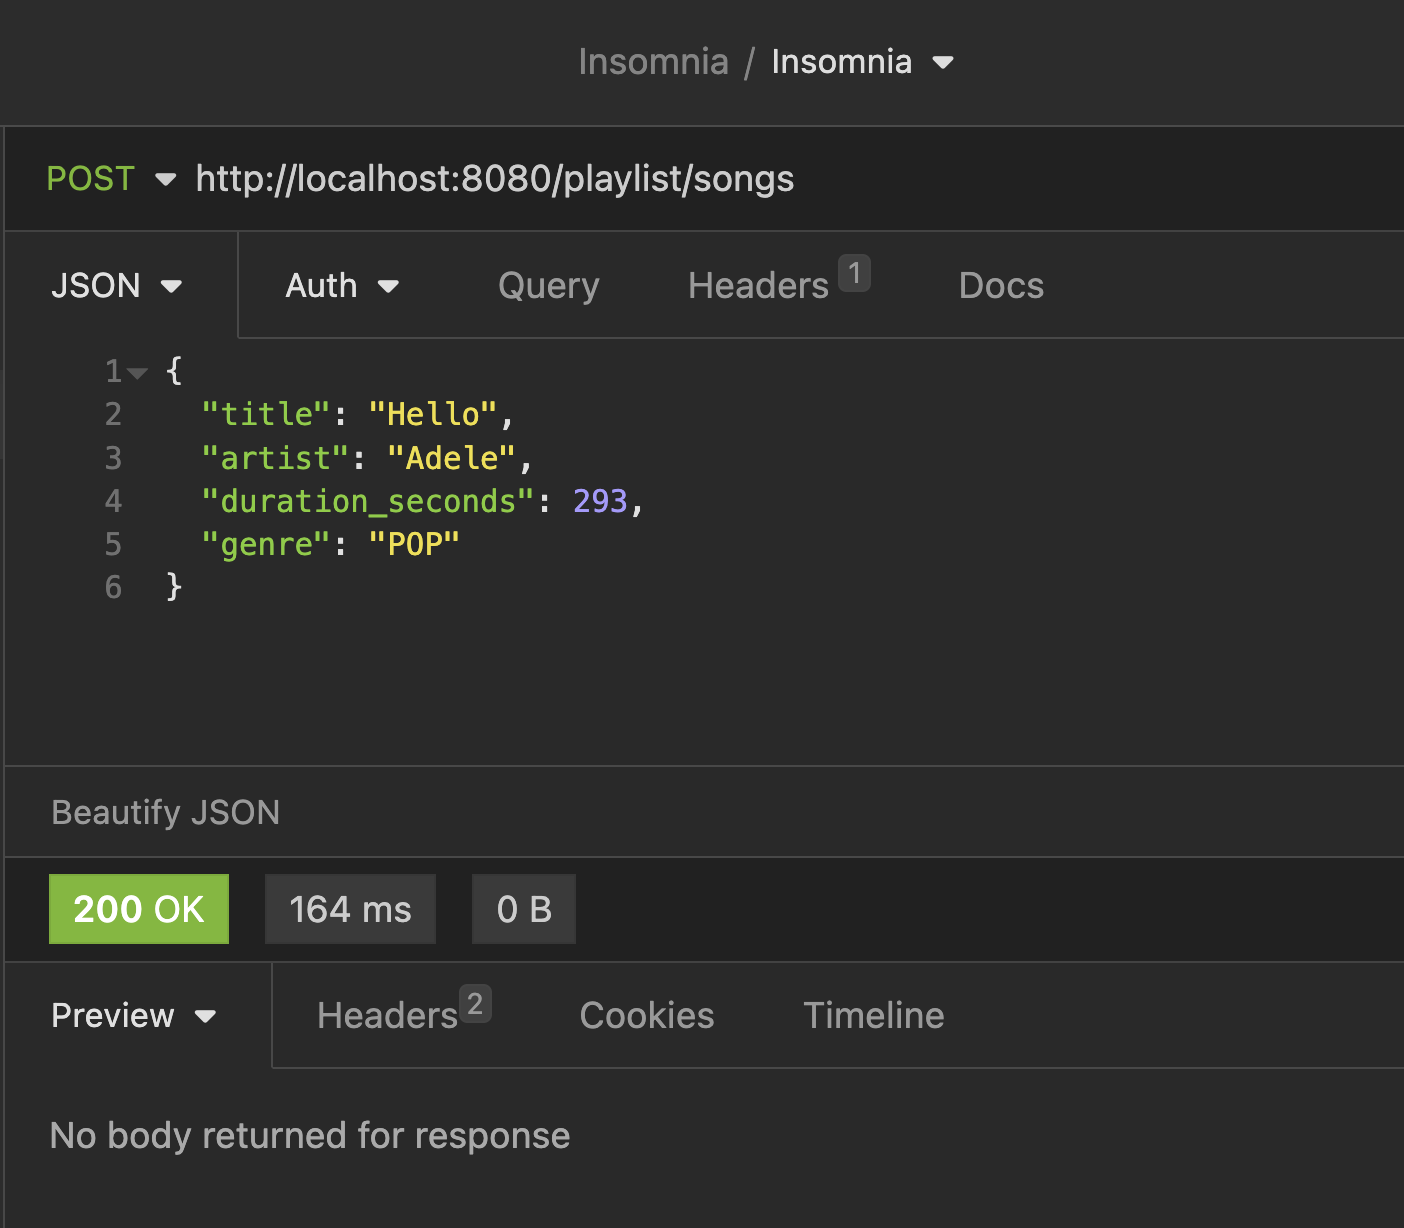
\includegraphics[width=\linewidth]{images/chapter-rest/insomnia_post.png}
  \caption{POST-verzoek met Insomnia}
  \label{fig:post_request}
\end{figure}

\subsection{De playlist opvragen}


\begin{apiRoute}{get}{/playlist/songs}{Retrieve all songs from the playlist}
\begin{routeParameter}
	\noRouteParameter {no parameter }
\end{routeParameter}
\begin{routeRequest}{application/json}
\end{routeRequest}
\begin{routeResponse}{application/json}
\begin{routeResponseItem}{200}{ok}
\begin{routeResponseItemBody}
[
	{
		"title": "Hello",
		"artist": "Adele",
		"genre": "POP",
		"duration_seconds": 293
	},
	{
		"title": "Shape of You",
		"artist": "Ed Sheeran",
		"genre": "POP",
		"duration_seconds": 233
	},
	{
		"title": "Umbrella",
		"artist": "Rihanna",
		"genre": "RNB",
		"duration_seconds": 264
	}
]
\end{routeResponseItemBody}
\end{routeResponseItem}
\end{routeResponse}
\end{apiRoute}


\begin{lstlisting}[language=java,  frame=single]
package be.pxl.demo;

import be.pxl.demo.domain.Song;
import org.springframework.stereotype.Service;

import java.util.ArrayList;
import java.util.List;

@Service
public class MusicPlaylistService {
	private final List<Song> myPlaylist = new ArrayList<>();

	public void addSong(Song song) {
		myPlaylist.add(song);
	}

	public List<Song> getSongs() {
		return myPlaylist;
	}
}
\end{lstlisting}


\begin{lstlisting}[language=java,  frame=single]
package be.pxl.demo.controller;

import be.pxl.demo.MusicPlaylistService;
import be.pxl.demo.domain.Song;
import org.slf4j.Logger;
import org.slf4j.LoggerFactory;
import org.springframework.beans.factory.annotation.Autowired;
import org.springframework.web.bind.annotation.GetMapping;
import org.springframework.web.bind.annotation.PostMapping;
import org.springframework.web.bind.annotation.RequestBody;
import org.springframework.web.bind.annotation.RequestMapping;
import org.springframework.web.bind.annotation.RestController;

import java.util.List;

@RestController
@RequestMapping("/playlist/songs")
public class MusicPlaylistController {

	private static final Logger LOGGER = LoggerFactory.getLogger(MusicPlaylistController.class);
	private final MusicPlaylistService musicPlaylistService;

	@Autowired
	public MusicPlaylistController(MusicPlaylistService musicPlaylistService) {
		this.musicPlaylistService = musicPlaylistService;
	}

	@PostMapping
	public void addSong(@RequestBody Song song) {
		if (LOGGER.isInfoEnabled()) {
			LOGGER.info("Adding song [" + song.getTitle() + "]");
		}
		musicPlaylistService.addSong(song);
	}

	@GetMapping
	public List<Song> getSongs() {
		return musicPlaylistService.getSongs();
	}
}
\end{lstlisting}

\subsection{Liedjes van \'e\'en genre}


 
 \begin{apiRoute}{get}{/playlist/songs/\{genre\}}{Retrieve all songs from the playlist with the given genre}
\begin{routeParameter}
	\routeParamItem{genre}{the requested genre}
\end{routeParameter}
\begin{routeRequest}{application/json}
\end{routeRequest}
\begin{routeResponse}{application/json}
\begin{routeResponseItem}{200}{ok}
\begin{routeResponseItemBody}
[
	{
		"title": "Hello",
		"artist": "Adele",
		"genre": "POP",
		"duration_seconds": 293
	},
	{
		"title": "Shape of You",
		"artist": "Ed Sheeran",
		"genre": "POP",
		"duration_seconds": 233
	}
]
\end{routeResponseItemBody}
\end{routeResponseItem}
\end{routeResponse}
\end{apiRoute}


\begin{lstlisting}[language=java,  frame=single]
package be.pxl.demo.controller;

import be.pxl.demo.MusicPlaylistService;
import be.pxl.demo.domain.Genre;
import be.pxl.demo.domain.Song;
import org.slf4j.Logger;
import org.slf4j.LoggerFactory;
import org.springframework.beans.factory.annotation.Autowired;
import org.springframework.web.bind.annotation.GetMapping;
import org.springframework.web.bind.annotation.PathVariable;
import org.springframework.web.bind.annotation.PostMapping;
import org.springframework.web.bind.annotation.RequestBody;
import org.springframework.web.bind.annotation.RequestMapping;
import org.springframework.web.bind.annotation.RestController;

import java.util.List;

@RestController
@RequestMapping("/playlist/songs")
public class MusicPlaylistController {

	private static final Logger LOGGER = LoggerFactory.getLogger(MusicPlaylistController.class);
	private final MusicPlaylistService musicPlaylistService;

	@Autowired
	public MusicPlaylistController(MusicPlaylistService musicPlaylistService) {
		this.musicPlaylistService = musicPlaylistService;
	}

	@PostMapping
	public void addSong(@RequestBody Song song) {
		if (LOGGER.isInfoEnabled()) {
			LOGGER.info("Adding song [" + song.getTitle() + "]");
		}
		musicPlaylistService.addSong(song);
	}

	@GetMapping
	public List<Song> getSongs() {
		return musicPlaylistService.getSongs();
	}

	@GetMapping("{genre}")
	public List<Song> getSongs(@PathVariable Genre genre) {
		return musicPlaylistService.getSongsByGenre(genre);
	}
}
\end{lstlisting}

\begin{lstlisting}[language=java,  frame=single]
package be.pxl.demo;

import be.pxl.demo.domain.Genre;
import be.pxl.demo.domain.Song;
import org.springframework.stereotype.Service;

import java.util.ArrayList;
import java.util.List;

@Service
public class MusicPlaylistService {
	private final List<Song> myPlaylist = new ArrayList<>();

	public void addSong(Song song) {
		myPlaylist.add(song);
	}

	public List<Song> getSongs() {
		return myPlaylist;
	}

	public List<Song> getSongsByGenre(Genre genre) {
		List<Song> response = new ArrayList<>();
		for (Song song : myPlaylist) {
			if (song.getGenre() == genre) {
				response.add(song);
			}
		}
		return response;
	}
}
\end{lstlisting}


\subsection{Gegevens van een liedje aanpassen}

Als je een nieuwe song in de playlist toevoegt, dan wordt deze steeds achteraan in de lijst toegevoegd. We kunnen nu de gegevens van het liedje op een gegeven positie in de lijst gaan overschrijven of aanpassen.  De index die we meegeven is een waarde van 0 tot 1 minder dan de lengte van de lijst.  Later zullen we zien hoe we een duidelijke foutboodschap kunnen geven aan de client als een foutieve index-waarde wordt gegeven.

Om de gegevens van een liedje aan te passen gebruiken we een PUT-verzoek. 
Je moet steeds alle gegevens van het liedje meegeven in de requestbody. 

\begin{apiRoute}{put}{/musicplaylist/songs\{index\}}{Update the song at the given index.}
\begin{routeParameter}
\routeParamItem{code}{unique identification of a house}
\end{routeParameter}
\begin{routeRequest}{application/json}
\begin{routeRequestBody}
{
		"title": "Hello",
		"artist": "Adele",
		"genre": "POP",
		"duration_seconds": 293
}
\end{routeRequestBody}
\end{routeRequest}
\begin{routeResponse}{application/json}
\begin{routeResponseItem}{200}{ok}
\end{routeResponseItem}
\end{routeResponse}
\end{apiRoute}


\begin{lstlisting}
package be.pxl.demo.controller;

import be.pxl.demo.MusicPlaylistService;
import be.pxl.demo.domain.Genre;
import be.pxl.demo.domain.Song;
import org.slf4j.Logger;
import org.slf4j.LoggerFactory;
import org.springframework.beans.factory.annotation.Autowired;
import org.springframework.web.bind.annotation.DeleteMapping;
import org.springframework.web.bind.annotation.GetMapping;
import org.springframework.web.bind.annotation.PathVariable;
import org.springframework.web.bind.annotation.PostMapping;
import org.springframework.web.bind.annotation.PutMapping;
import org.springframework.web.bind.annotation.RequestBody;
import org.springframework.web.bind.annotation.RequestMapping;
import org.springframework.web.bind.annotation.RestController;

import java.util.List;

@RestController
@RequestMapping("/playlist/songs")
public class MusicPlaylistController {

	private static final Logger LOGGER = LoggerFactory.getLogger(MusicPlaylistController.class);
	private final MusicPlaylistService musicPlaylistService;

	@Autowired
	public MusicPlaylistController(MusicPlaylistService musicPlaylistService) {
		this.musicPlaylistService = musicPlaylistService;
	}

	@PostMapping
	public void addSong(@RequestBody Song song) {
		if (LOGGER.isInfoEnabled()) {
			LOGGER.info("Adding song [" + song.getTitle() + "]");
		}
		musicPlaylistService.addSong(song);
	}

	@GetMapping
	public List<Song> getSongs() {
		return musicPlaylistService.getSongs();
	}

	@GetMapping("/{genre}")
	public List<Song> getSongs(@PathVariable Genre genre) {
		return musicPlaylistService.getSongsByGenre(genre);
	}

	@PutMapping("/{index}")
	public void updateSong(@PathVariable int index, @RequestBody Song song) {
		musicPlaylistService.updateSong(index, song);
	}
}
\end{lstlisting}

\begin{lstlisting}
package be.pxl.demo;

import be.pxl.demo.domain.Genre;
import be.pxl.demo.domain.Song;
import org.springframework.stereotype.Service;

import java.util.ArrayList;
import java.util.List;

@Service
public class MusicPlaylistService {
	private final List<Song> myPlaylist = new ArrayList<>();

	public void addSong(Song song) {
		myPlaylist.add(song);
	}

	public List<Song> getSongs() {
		return myPlaylist;
	}

	public List<Song> getSongsByGenre(Genre genre) {
		List<Song> response = new ArrayList<>();
		for (Song song : myPlaylist) {
			if (song.getGenre() == genre) {
				response.add(song);
			}
		}
		return response;
	}

	public void updateSong(int index, Song song) {
		myPlaylist.set(index, song);
	}

	public void deleteSong(int index) {
		myPlaylist.remove(index);
	}
}
\end{lstlisting}

We vervangen het liedje op de opgegeven index door een nieuw Song-object met de aangepaste gegevens.

\subsection{Een liedje verwijderen}

Om een liedje op een opgegeven index uit de playlist te verwijderen gaan we een DELETE-verzoek implementeren.


\begin{apiRoute}{delete}{/musicplaylist/songs/\{index\}}{Delete the song at the given index.}
\begin{routeParameter}
\routeParamItem{index}{position of the song to be deleted}
\end{routeParameter}
\begin{routeResponse}{application/json}
\begin{routeResponseItem}{200}{ok}
\end{routeResponseItem}
\end{routeResponse}
\end{apiRoute}

\begin{lstlisting}
package be.pxl.demo.controller;

import be.pxl.demo.MusicPlaylistService;
import be.pxl.demo.domain.Genre;
import be.pxl.demo.domain.Song;
import org.slf4j.Logger;
import org.slf4j.LoggerFactory;
import org.springframework.beans.factory.annotation.Autowired;
import org.springframework.web.bind.annotation.DeleteMapping;
import org.springframework.web.bind.annotation.GetMapping;
import org.springframework.web.bind.annotation.PathVariable;
import org.springframework.web.bind.annotation.PostMapping;
import org.springframework.web.bind.annotation.PutMapping;
import org.springframework.web.bind.annotation.RequestBody;
import org.springframework.web.bind.annotation.RequestMapping;
import org.springframework.web.bind.annotation.RestController;

import java.util.List;

@RestController
@RequestMapping("/playlist/songs")
public class MusicPlaylistController {

	private static final Logger LOGGER = LoggerFactory.getLogger(MusicPlaylistController.class);
	private final MusicPlaylistService musicPlaylistService;

	@Autowired
	public MusicPlaylistController(MusicPlaylistService musicPlaylistService) {
		this.musicPlaylistService = musicPlaylistService;
	}

	@PostMapping
	public void addSong(@RequestBody Song song) {
		if (LOGGER.isInfoEnabled()) {
			LOGGER.info("Adding song [" + song.getTitle() + "]");
		}
		musicPlaylistService.addSong(song);
	}

	@GetMapping
	public List<Song> getSongs() {
		return musicPlaylistService.getSongs();
	}

	@GetMapping("/{genre}")
	public List<Song> getSongs(@PathVariable Genre genre) {
		return musicPlaylistService.getSongsByGenre(genre);
	}

	@PutMapping("/{index}")
	public void updateSong(@PathVariable int index, @RequestBody Song song) {
		musicPlaylistService.updateSong(index, song);
	}

	@DeleteMapping("/{index}")
	public void updateSong(@PathVariable int index) {
		musicPlaylistService.deleteSong(index);
	}
}
\end{lstlisting}


\begin{lstlisting}
package be.pxl.demo;

import be.pxl.demo.domain.Genre;
import be.pxl.demo.domain.Song;
import org.springframework.stereotype.Service;

import java.util.ArrayList;
import java.util.List;

@Service
public class MusicPlaylistService {
	private final List<Song> myPlaylist = new ArrayList<>();

	public void addSong(Song song) {
		myPlaylist.add(song);
	}

	public List<Song> getSongs() {
		return myPlaylist;
	}

	public List<Song> getSongsByGenre(Genre genre) {
		List<Song> response = new ArrayList<>();
		for (Song song : myPlaylist) {
			if (song.getGenre() == genre) {
				response.add(song);
			}
		}
		return response;
	}

	public void updateSong(int index, Song song) {
		myPlaylist.set(index, song);
	}

	public void deleteSong(int index) {
		myPlaylist.remove(index);
	}
}
\end{lstlisting}


\begin{oefening}\textbf{Huizenjacht}
We maken een Spring Boot toepassing om het aanbod op de huizenmarkt te beheren.
Ontwikkel een RESTful web toepassing met onderstaande endpoints.
Je voorziet een component HouseService met \'e\'en enkele, gedeelde lijst van woningen  voor alle gebruikers.

Een huis wordt voorgesteld als een resource met volgende eigenschappen:

\begin{itemize}
  \item \texttt{code} (string): Unieke identificatie van het huis.
  \item \texttt{name} (string): Naam of beschrijving van het huis.
  \item \texttt{status} (enum): Status FOR\_SALE of SOLD.
  \item \texttt{city} (string): Locatie van het huis.
  \item \texttt{price} (double): Prijs van het huis.
\end{itemize}

\section{REST Endpoints}

\begin{apiRoute}{post}{/houses}{Create a new house.}
\begin{routeParameter}
	\noRouteParameter {no parameter }
\end{routeParameter}
\begin{routeRequest}{application/json}
\begin{routeRequestBody}
{
  "code": "HAS_001",
  "name": "Beautiful house in the city",
  "city": "Hasselt",
  "price": 250000
}
\end{routeRequestBody}
\end{routeRequest}
\begin{routeResponse}{application/json}
\begin{routeResponseItem}{200}{ok}
\end{routeResponseItem}
\end{routeResponse}
\end{apiRoute}


\begin{apiRoute}{put}{/houses/\{code\}}{Update the data (status, price,...) of the house with the given code.}
\begin{routeParameter}
\routeParamItem{code}{unique identification of a house}
\end{routeParameter}
\begin{routeRequest}{application/json}
\begin{routeRequestBody}
{
  "status": "SOLD"
  "name": "Beautiful house in the city",
  "price": 320000
}
\end{routeRequestBody}
\end{routeRequest}
\begin{routeResponse}{application/json}
\begin{routeResponseItem}{200}{ok}
\end{routeResponseItem}
\end{routeResponse}
\end{apiRoute}

\begin{apiRoute}{get}{/houses}{Retrieve all houses.}
\begin{routeParameter}
	\noRouteParameter {no parameter }
\end{routeParameter}
\begin{routeResponse}{application/json}
\begin{routeResponseItem}{200}{ok}
\begin{routeResponseItemBody}
[
  {
    "code": "GNK_001",
    "name": "Beautiful house in the city",
    "status": "SOLD",
     "city": "Genk",
    "price": 250000
  },
  {
    "code": "HAS_003",
    "name": "Cozy bungalow",
    "status": "FOR_SALE",
     "city": "Hasselt",
    "price": 180000
  }
]
\end{routeResponseItemBody}
\end{routeResponseItem}
\end{routeResponse}
\end{apiRoute}

\begin{apiRoute}{delete}{/houses/\{code\}}{Delete the house with the given code.}
\begin{routeParameter}
\routeParamItem{code}{unique identification of a house}
\end{routeParameter}
\begin{routeResponse}{application/json}
\begin{routeResponseItem}{200}{ok}
\end{routeResponseItem}
\end{routeResponse}
\end{apiRoute}

\end{oefening}

\chapter{Collections: Map}

In Java is de \textit{Map} interface een onderdeel van het Java Collections Framework. 
Je gebruikt deze gegevensstructuur als je key-value paren (sleutel-waarde paren) wilt opslaan en beheren.  De unieke sleutel wordt opgeslaan en gekoppeld aan een specifieke waarde.  De belangrijkste implementaties van de Map interface in Java zijn HashMap, LinkedHashMap, TreeMap en Hashtable.

\section{Generieke klasse HashMap}

De interface Map en de klasse HashMap zijn generiek.  Dit betekent dat ze zijn ontworpen om met verschillende datatypes te werken, zonder het datatype op voorhand vast te leggen. In het geval van HashMap, maakt het gebruik van generieke datatypes het mogelijk om de key- en value-datatypen flexibel te kiezen op het moment dat je een instantie van de HashMap maakt. Hierdoor kun je de HashMap gebruiken met verschillende soorten gegevens zonder dat je aparte klassen hoeft te schrijven voor elke combinatie van datatypes.

HashMap<K, V>

K staat voor het datatype van de sleutels die je in de HashMap wilt opslaan.
V staat voor het datatype van de waarden die je in de HashMap wilt opslaan.

\section{De interface Map}

Hier is een overzicht van enkele veelgebruikte methoden in de Map interface:

\begin{itemize}
\item \textbf{put(K key, V value)} Voegt een sleutel-waarde paar toe aan de map.
\item \textbf{get(K key)} Geeft de waarde terug die is gekoppeld aan de opgegeven sleutel, of null als de sleutel niet in de map voorkomt.
\item \textbf{containsKey(K key)} Controleert of de map een specifieke sleutel bevat.
\item \textbf{containsValue(V value)} Controleert of de map een specifieke waarde bevat.
\item \textbf{remove(K key)} Verwijdert de opgegeven sleutel met zijn gekoppelde waarde.
\item \textbf{keySet()} Geeft een lijst (List) van alle sleutels in de map terug.
\item \textbf{values()} Geeft een lijst (List) van alle waarden in de map terug.
\end{itemize}



\section{Gebruik van HashMap}

\subsection{Voorbeeld 1}

\begin{lstlisting}
import java.util.HashMap;
import java.util.Map;

public class HashMapVoorbeeld {
    public static void main(String[] args) {
        // Een HashMap maken met String sleutels en Integer waarden
        Map<String, Integer> scores = new HashMap<>();

        // Sleutel-waarde paren toevoegen
        leeftijden.put("Alice", 25);
        leeftijden.put("Bob", 30);
        leeftijden.put("Charlie", 28);
        leeftijden.put("David", 35);

        // Waarde ophalen op basis van een sleutel
        int scoreVanAlice = scores.get("Alice");
        System.out.println("Score van Alice: " + scoreVanAlice); // Geeft 25 weer

        // Controleren of een sleutel aanwezig is
        boolean bevatSleutel = scores.containsKey("Eve");
        System.out.println("Bevat sleutel 'Eve': " + bevatSleutel); // Geeft false weer

        // Sleutel-waarde paar verwijderen
        scores.remove("Bob");

        // Alle sleutels afdrukken
        System.out.println("Sleutels in de map: " + scores.keySet()); 
        // geeft [Alice, Charlie, David]

        // Alle waarden afdrukken
        System.out.println("Waarden in de map: " + scores.values()); 
        // geeft [25, 28, 35]
    }
}
\end{lstlisting}

\subsection{Voorbeeld 2}

In dit voorbeeld maken we voor de sleutel-waarden gebruik van Strings. Voor de waarden gebruiken we een zelfgedefinieerde klasse, in dit geval de klasse Player. 
Op deze manier kunnen we dus heel gemakkelijk het juiste Player-object opzoeken en eventueel de score aanpassen als we de naam van de speler kennen.

\begin{lstlisting}

import java.util.HashMap;
import java.util.Map;

public class Player {
    private String naam;
    private int score;

    public Player(String naam, int score) {
        this.naam = naam;
        this.score = score;
    }

    public String getNaam() {
        return naam;
    }

    public int getScore() {
        return score;
    }
    
    public void setScore(int score) {
    		this.score = score;
    }
}
\end{lstlisting}


\begin{lstlisting}
public class SpelerHashMap {
    public static void main(String[] args) {
        // Een HashMap maken met String-sleutels en Player-waarden
        Map<String, Player> spelerMap = new HashMap<>();

        // Spelers toevoegen
        spelerMap.put("Alice", new Player("Alice", 100));
        spelerMap.put("Bob", new Player("Bob", 85));
        spelerMap.put("Charlie", new Player("Charlie", 92));

        // Spelersinformatie ophalen op basis van naam
        String spelerNaam = "Bob";
        Player speler = spelerMap.get(spelerNaam);
        System.out.println("Speler " + spelerNaam + " heeft een score van " + speler.getScore());
    }
}
\end{lstlisting}


\begin{oefening}\textbf{Huizenjacht v2}
Pas de oefening Huizenjacht uit het vorige hoofdstuk aan. In de service-laag gebruik je een HashMap zodat je een huis heel eenvoudig kunt opzoeken als je de code kent.
\end{oefening}

\chapter{Foutafhandeling}

\begin{summary}
Tijdens het uitvoeren van een programma kan en zal er vanalles foutgaan. De gebruiker van het programma geeft de datum in in een foutief formaat, een printer is offline, er is onvoldoende schrijfruimte vrij om een bestand weg te schrijven, het programma kreeg onvoldoende geheugen toegewezen,... Fouten die zich voordoen tijdens het uitvoeren van een programma, at runtime dus, verdelen we onder in errors en exceptions. Errors zijn de fouten die meestal veroorzaakt worden door het onderliggende besturingssysteem. Tijdens het verloop van het programma kunnen deze errors niet meer opgelost worden en het programma zal daarom be\"eindigd worden. Dit is niet het geval voor exceptions. Je kan je code op een defensieve manier schrijven en rekening houden met de mogelijke exceptions die kunnen optreden. ``Exception handling'' is het proces om deze exceptions op een correcte en liefst gebruiksvriendelijke manier af te handelen. Indien een fout niet correct wordt afgehandeld, zal het programma alsnog voortijdig afgebroken worden, maar met de juiste foutafhandeling kan de uitvoer van het programma gewoon verdergezet worden. 
 \end{summary}
 
\section{Compile-time vs runtime errors}

Een programmeur schrijft Java code in zijn editor of favoriete IDE. Vervolgens wordt de Java code gecompileerd tot bytecode. Deze bytecode wordt door de JVM (Java Virtual Machine) ge\"interpreteerd tot machinecode instructies die worden uitgevoerd door het computersysteem.

Wanneer dus een Java programma wordt opgestart, kunnen er 2 categorie\"en van problemen voorkomen. Het kan zijn dat het Java programma niet gecompileerd kan worden. In dat geval spreken we van een compile-time error. Indien het programma succesvol gecompileerd wordt, kan er zich tijdens het uitvoeren van de code een probleem voordoen, in dat geval spreken we van runtime errors of exceptions. 

\begin{figure}[H]
  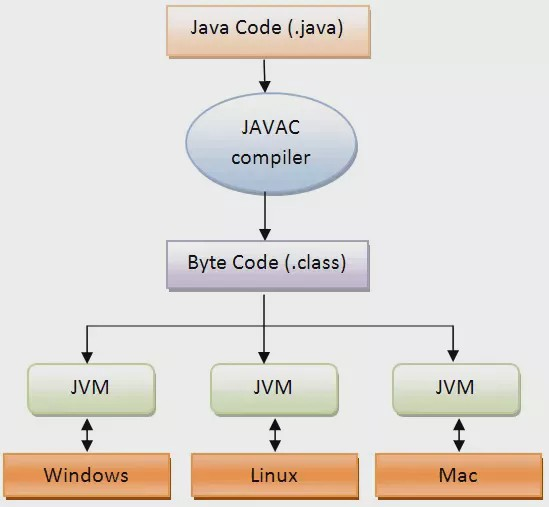
\includegraphics[width=\linewidth]{images/h1/java_compiler.jpeg}
  \caption{Compiler, interpreter en Java Virtual Machine.}
  \label{fig:compiler}
\end{figure}


\begin{figure}[H]
  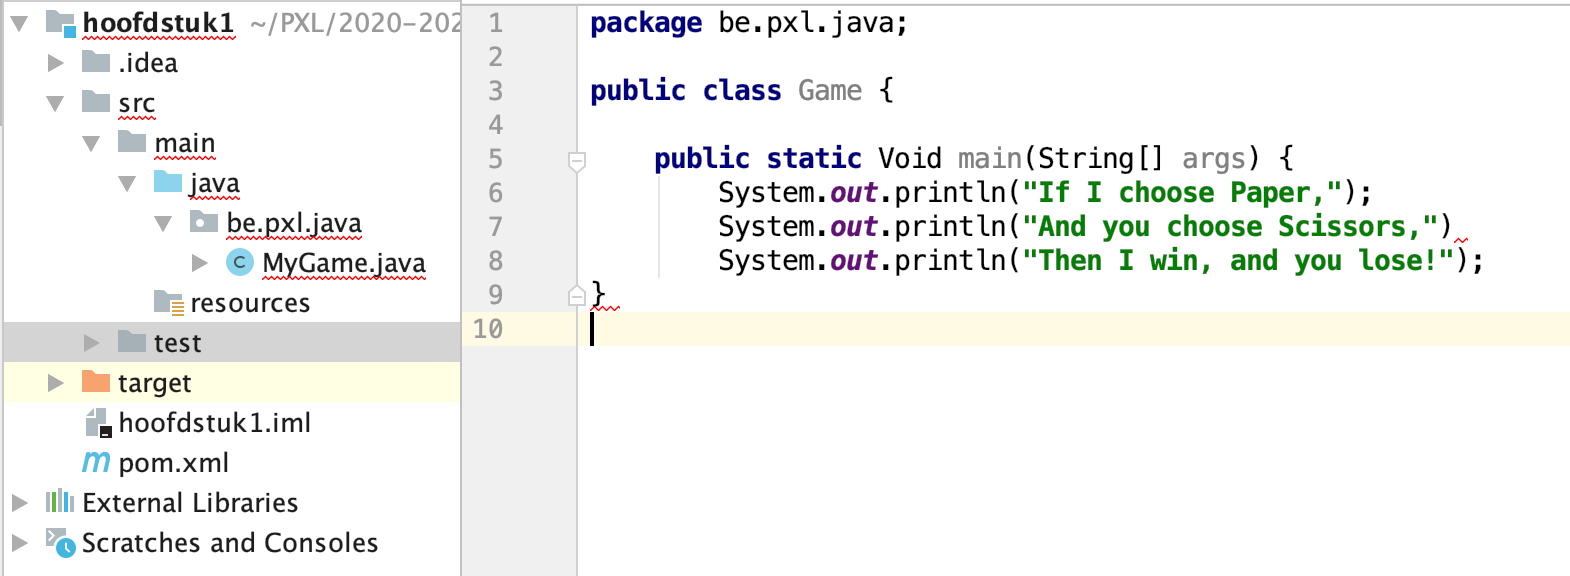
\includegraphics[width=\linewidth]{images/h1/compiletime_errors.png}
  \caption{Compile-time errors}
  \label{fig:compiletime_errors}
\end{figure}

\begin{oefening}
Welke compile-time errors kan je ontdekken in het volgende codefragment in figuur \ref{fig:compiletime_errors}?
\end{oefening}

Omdat Java een object-ge\"orienteerde programmeertaal is, wordt er ook een object gebruikt om aan te geven dat er iets fout ging bij uitvoeren van het Java programma. Zodra er zich een probleem voordoet tijdens het uitvoeren van een programma-instructie, wordt er een exception-object aangemaakt en ``opgeworpen''. Hierdoor stopt de normale uitvoer van het programma. Er wordt nog geprobeerd om het exception-object op een keurige manier af te handelen (indien die code aanwezig is), maar als dat niet lukt zal het programma be\"eindigd worden. Het exception-object bevat nuttige informatie voor de ontwikkelaar zoals de methode en lijn-nummer waar de exception werd aangemaakt en het type van de exception. 

\section{First catch}

\begin{lstlisting}
public class DivisionByZero {

	public static void main(String[] args) {
		int a = (1 + 1) % 2;
		int b = 5;
		int c = b / a;
		System.out.println("Het resultaat is " + c);
	}
}
\end{lstlisting}

Als je het bovenstaande programma uitvoert zal het volgende in de console verschijnen:

\begin{verbatim}
Exception in thread "main" java.lang.ArithmeticException: / by zero
	at be.pxl.ja.DivisionByZero.main(DivisionByZero.java:6)<5 internal calls>
\end{verbatim}
  
De variabele \textit{a} bevat inderdaad de waarde 0 en hierdoor hebben we dus te maken met een deling door 0. Zodra de deling wordt uitgevoerd loopt het dus fout en gooit de java runtime een ArithmeticException op. Omdat de ArithmeticException nergens wordt afgehandeld eindigt het programma. Je zal enkel nog een stacktrace zien verschijnen in de console. Een stacktrace is de naam en foutboodschap van de exception gevolgd door de weg die de exception heeft afgelegd (doorheen de methoden van je klassen) vanaf het moment dat ze werd opgegooid. We zien dus dat de exception is veroorzaakt op regel 6 in de klasse DivisionByZero.

\begin{lstlisting}
public class DivisionByZero {

	public static void main(String[] args) {
		int a = (1 + 1) % 2;
		int b = 5;
		try {
			int c = b / a;
			System.out.println("Het resultaat is " + c);
		} catch (ArithmeticException e) {
			System.out.println("You should not divide a number by zero.");
		}
		System.out.println("First catch completed!");
	}
}
\end{lstlisting}

\begin{verbatim}
You should not divide a number by zero.
First catch completed!
\end{verbatim}

We hebben de instructie met de deling nu in een try-blok geplaatst. Omdat de variabele c in het try-blok wordt aangemaakt, kan deze variabele ook enkel binnen het try-blok gebruikt worden. Indien een exception optreedt binnen een try-blok zal de programma-uitvoer de resterende code binnen het try-blok overslaan en verdergaan bij het eerste catch-blok dat direct volgt achter het try-blok. Je bent als programmeur verplicht om een try-blok steeds te laten volgen door \'e\'en of meerdere catch-blokken.
In het catch-blok wordt dan de code uitgevoerd om het probleem op te lossen of tenminste een duidelijke boodschap voor de gebruiker van het programma te voorzien.
Als alle instructies uit het catch-blok zijn uitgevoerd zal het programma zijn normale uitvoer verderzetten.


\section{Java exception hi\"erarchie}
  
\begin{figure}[H]
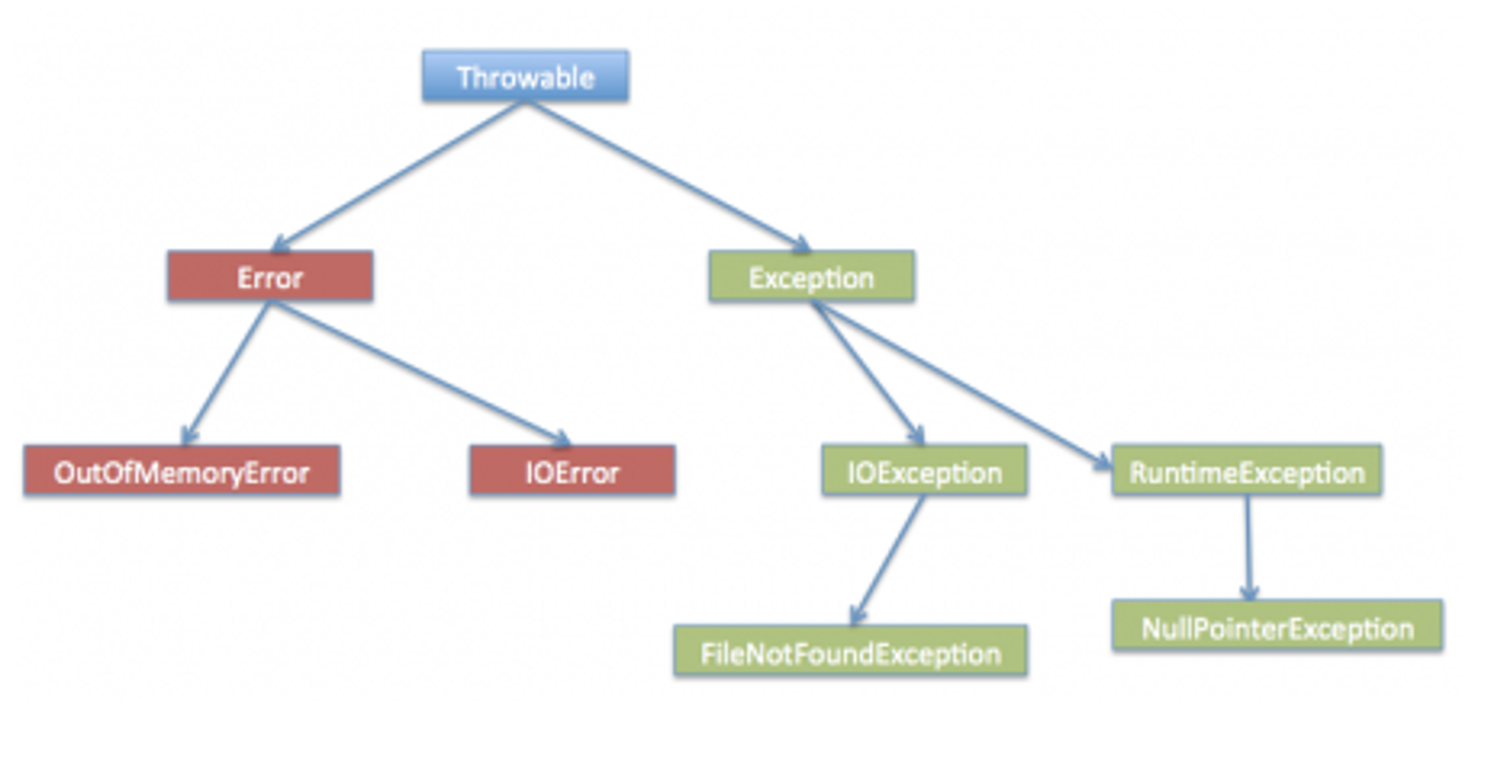
\includegraphics[width=\linewidth]{images/h1/exception-hierarchy.png}
\caption{Exception hi\"erarchie}
\label{fig:exceptiono_hierarchy}
\end{figure}
  
Zoals reeds vermeld wordt er een exception-object aangemaakt zodra zich een probleem voordoet in de code. 
Er is in Java een hi\"erarchie gebouwd van exception-klassen om verschillende soorten fouten in een programma te categorizeren. Throwable is de superklasse van alle exceptions en errors in Java. Er zijn dus 2 afgeleide klassen van Throwable: Error and Exception. Exceptions zijn nog verder onderverdeeld in \textbf{checked exceptions} en \textbf{runtime exceptions}.

\subsection{Errors}

Errors zijn problemen die zich voordoen tijdens het uitvoeren van het programma en die meestal niet gerelateerd zijn aan het programma zelf. Daarom is het onmogelijk om erop te anticiperen en te herstellen van deze fouten. Dit kan gaan van hardware falen, over JVM crashes en out of memory errors. We hebben een aparte hi\"erarchie van errors en we zullen nooit code toevoegen in ons programma om deze fouten af te handelen. We tonen hier enkel voorbeelden van errors.


\subsubsection{StackOverflowError}
Je hebt ongetwijfeld al eens per ongeluk een programma geschreven met een oneindige lus. 

\begin{lstlisting}
public class DemoStackOverflow {

	private static void printNumber(int x) {
		System.out.println(x);
		printNumber(x + 2);
	}

	public static void main(String[] args) {
		printNumber(15);
	}
}
\end{lstlisting}

\begin{verbatim}
15
17
19
...
36597
36599
Exception in thread "main" java.lang.StackOverflowError
	...
	at be.pxl.ja.DemoStackOverflow.printNumber(DemoStackOverflow.java:5)
	at be.pxl.ja.DemoStackOverflow.printNumber(DemoStackOverflow.java:5) 
	at be.pxl.ja.DemoStackOverflow.printNumber(DemoStackOverflow.java:5) 
	at be.pxl.ja.DemoStackOverflow.printNumber(DemoStackOverflow.java:5) 
	...
\end{verbatim}

De call stack is de manier waarop tijdens de uitvoer van een programma o.a. wordt bijgehouden welke functies worden aangeroepen. Wanneer je programma-uitvoer in een oneindige lus terechtkomt, stapelen de gegevens in de call stack zich razendsnel op en loopt de call stack vol. Het programma zal uiteindelijk eindigen met een StackOverflowError.

\begin{figure}[H]
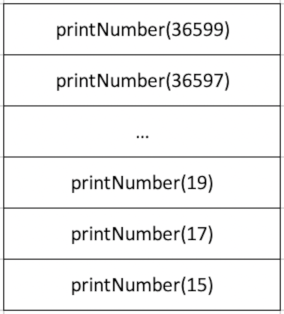
\includegraphics{images/h2/java_call_stack.png}
\caption{Java call stack}
\label{fig:call_stack}
\end{figure}


\subsubsection{OutOfMemoryError}

\begin{lstlisting}
public class DemoOutOfMemory {

	private void generateOutOfMemory() {
		Long maxMemory = Runtime.getRuntime().maxMemory();
		System.out.println(maxMemory);

		int[] matrix = new int[(int) (maxMemory + 1)];
		for (int i = 0; i < matrix.length; ++i) {
			matrix[i] = i + 1;
		}
		System.out.println("Matrix filled" + matrix[(int)(Math.random() * 100)]);

	}

	public static void main(String[] args) {
		DemoOutOfMemory doom = new DemoOutOfMemory();
		doom.generateOutOfMemory();
	}
}
\end{lstlisting}

Om de OutOfMemoryError te illustreren maken we een array aan die meer geheugenplaatsen inneemt dan de ruimte die het java programma ter beschikking heeft.

Als je dit programma uitvoert, pas je best het beschikbare geheugen voor het programma aan. Dit doe je door een waarde voor de VM optie -Xmx mee te geven.

\begin{itemize}
\item -Xmssize: Geeft de initi\"ele waarde voor de heap size.
\item -Xmxsize: Geeft de maximale waarde voor heap size.
\end{itemize}

De heap size van een Java programma is de hoeveelheid geheugen dat een Java-programma mag gebruiken om objecten op te slaan.

\begin{verbatim}
67108864
Exception in thread "main" java.lang.OutOfMemoryError: Java heap space
	at be.pxl.ja.DemoOutOfMemory.generateOutOfMemory(DemoOutOfMemory.java:8)
	at be.pxl.ja.DemoOutOfMemory.main(DemoOutOfMemory.java:16)<5 internal calls>
\end{verbatim}
	
\begin{figure}[H]
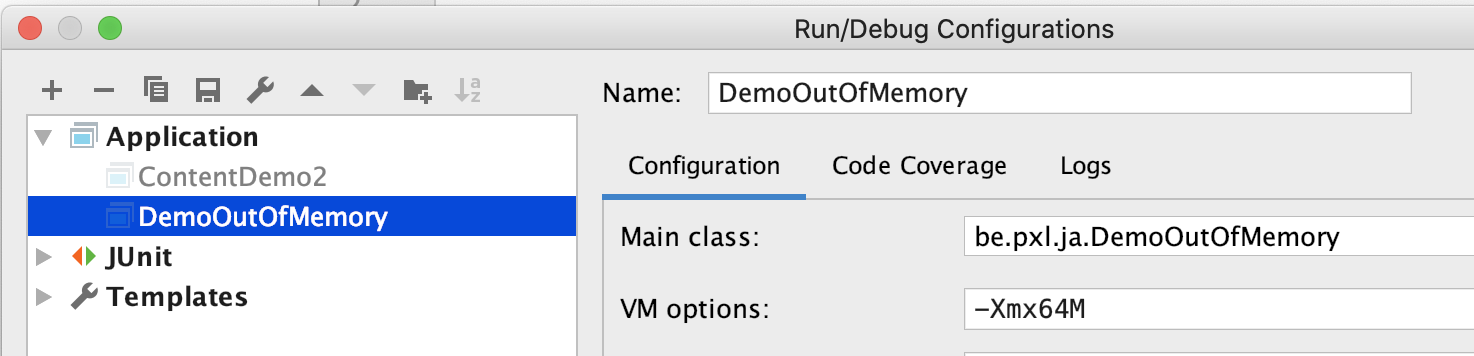
\includegraphics[width=\linewidth]{images/h2/jvm_options_xmx.png}
\caption{Maximum heap size aanpassen}
\label{fig:exceptiono_hierarchy}
\end{figure}

\subsection{Runtime exceptions}

Runtime exceptions zijn exceptions die vaak veroorzaakt worden door logische fouten in het programma.Typische voorbeelden van runtime exceptions zijn ArrayIndexOutOfBoundsException, NullPointerException en IllegalArgumentException. Vaak moet je ze niet afhandelen, maar moet je ervoor zorgen dat je de bug in je code oplost. Ook hier zijn onze unit testen heel belangrijk. Door goede unit testen te schrijven ga je runtime exceptions in je code opmerken en kunnen oplossen.

\begin{lstlisting}
public class Demo {

	public static void main(String[] args) {
		String tekst = "abc";
		System.out.println(tekst.repeat(-5));
	}
}
\end{lstlisting}

\begin{verbatim}
Exception in thread "main" java.lang.IllegalArgumentException: count is negative: -5
	at java.base/java.lang.String.repeat(String.java:3586)
	at be.pxl.ja.streamingservice.Demo.main(Demo.java:5)
\end{verbatim}

\begin{oefening}

\begin{lstlisting}
public class StreamingService {

	private List<Account> accounts;

	public void addAccount(Account account) {
		accounts.add(account);
	}
}
\end{lstlisting}

Welke exception doet zich voor zodra je voor een object van de klasse StreamingService de methode addAccount() aanroept? Waarom treedt die exception op?
\end{oefening}

Wanneer je programma gebruikmaakt van gegevens die door de gebruiker worden ingevoerd, moet je er altijd rekening mee houden dat de gebruiker foutieve gegevens kan ingeven. Deze foutieve gegevens kunnen aanleiding geven tot runtime exceptions. Ook hier moet je steeds anticiperen op de mogelijke input die de gebruiker kan invoeren. 


\begin{lstlisting}
public class ElementInArray {

	public static void main(String[] args) {
		String[] elements = { "H", "He", "Li", "Be", "B", "C", "N", "O", "F", "Ne" };

		Scanner scanner = new Scanner(System.in);
		
		// OPLOSSING 1
		System.out.println("Kies een nummer: ");
		int chosen = scanner.nextInt();
		if (chosen < elements.length) {
			System.out.println(elements[chosen]);
		} else {
			System.out.println("U koos een verkeerd nummer.");
		}

	    // OPLOSSING 2
		System.out.println("Kies een nummer: ");
		chosen = scanner.nextInt();
		try {
			System.out.println(elements[chosen]);
		} catch (ArrayIndexOutOfBoundsException e) {
			System.out.println("U koos een verkeerd nummer.");
		}
	}
}
\end{lstlisting}

In bovenstaand codevoorbeeld gaat onze voorkeur uit naar oplossing 1 waarbij de ingevoerde waarde wordt gecontroleerd vooraleer het element uit de array wordt benaderd. Deze code is makkelijker leesbaar en onderhoudbaar.

\begin{oefening}
Maak een programma dat de geboortedatum vraagt als input. Vervolgens berekent het programma hoeveel dagen het nog duurt vooraleer je jarig bent. Gebruik de methode parse() uit de klasse LocalDateTime om van de input van de gebruiker een LocalDateTime-object te maken. Welke exception kan optreden? Blijf input vragen totdat de gebruiker een correcte datum heeft ingegeven.
\end{oefening}


\subsection{Checked exceptions}

Wanneer je in java een methode aanroept, kan het voorkomen dat je direct een compileerfout voorgeschoteld krijgt. Het kan namelijk zijn dat java reeds anticipeert op mogelijke problemen en je dwingt om rekening te houden met het scenario dat er iets mis kan gaan. De compileerfout raakt pas opgelost wanneer je het afhandelen van de exception netjes programmeert.

Kijk eens naar onderstaand voorbeeld uit de streaming service.
We gebruiken hier de klasse MessageDigest uit JDK. Message digests zijn functies waarmee we voor input-data van willekeurige lengte een hash-waarde met een vaste lengte kunnen berekenen.  Als je de hash-waarde kent, kan je hieruit de input-data niet afleiden. We gebruiken dit om een paswoord bij te houden in een Account-object. We willen absoluut vermijden dat paswoorden in een leesbaar formaat in onze objecten worden bijgehouden.

Om een message digest te berekenen in Java moet je eerst de static methode getInstance() aanroepen met als parameter het door jouw gekozen algoritme. In dit voorbeeld wordt er gekozen voor MD5. Je ziet dat de lijn code, ondanks het feit dat alles correct is geschreven, toch rood wordt onderlijnd. Dat komt omdat de methode getInstance() een exception kan opgooien die we verplicht moeten afhandelen.

\begin{oefening}
Open de documentatie van de klasse MessageDigest en bekijk de uitleg voor de static methode getInstance(). Kan je hier zien welke exceptions er kunnen voorkomen?
\end{oefening}

\begin{figure}[H]
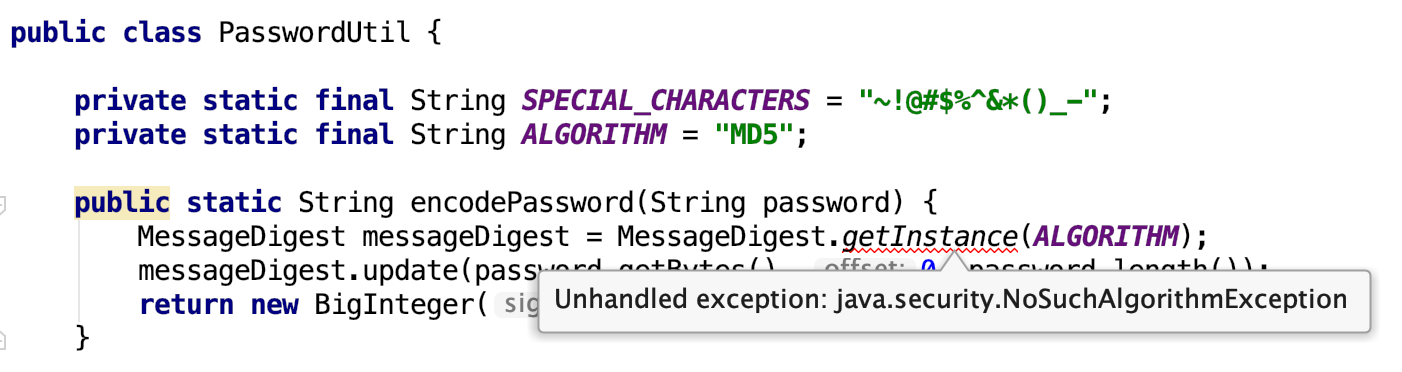
\includegraphics[width=\linewidth]{images/h2/no_such_algorithm_exception.png}
\caption{Een checked exception: NoSuchAlgorithmException}
\label{fig:no_such_algorithm}
\end{figure}

Deze compileerfout wordt veroorzaakt omdat de exception-klasse NoSuchAlgorithmException een checked exception is. Dit betekent dat het aanroepen van de methode die de exception gooit een compileerfout zal geven, omdat er geen code is toegevoegd om correct met de  exception om te gaan.
Er zijn 2 mogelijke oplossingen om deze compileerfout aan te pakken. Ofwel vang de exception op en handel je ze af in de methode encodePassword(), ofwel voeg je in de signatuur van de methode encodePassword() toe dat je de methode toelaat om een NoSuchAlgorithmException op te werpen. We geven nu eerst een voorbeeld van hoe je de exception kan opvangen en afhandelen. 

\begin{lstlisting}
import be.pxl.ja.streamingservice.util.PasswordUtil;

public class Account {
	private String email;
	private String password;

	public Account(String email, String password) {
		this.email = email;
		setPassword(password);
	}

	public String getEmail() {
		return email;
	}

	public void setEmail(String email) {
		this.email = email;
	}

	public boolean verifyPassword(String password) {
		return PasswordUtil.isValid(password, this.password);
	}

	public void setPassword(String password) {
		this.password = PasswordUtil.encodePassword(password);
	}
}
\end{lstlisting}

\begin{lstlisting}
import java.math.BigInteger;
import java.security.MessageDigest;
import java.security.NoSuchAlgorithmException;

public class PasswordUtil {

	private static final String ALGORITHM = "MD5";

	public static String encodePassword(String password) {
		MessageDigest messageDigest = null;
		try {
			messageDigest = MessageDigest.getInstance(ALGORITHM);
		} catch (NoSuchAlgorithmException e) {
			return null;
		}
		messageDigest.update(password.getBytes(), 0, password.length());
		return new BigInteger(1, messageDigest.digest()).toString(16);
	}

	public static boolean isValid(String providedPassword, String securedPassword) {
		return encodePassword(providedPassword).equals(securedPassword);
	}
}
\end{lstlisting}


\begin{lstlisting}
import be.pxl.ja.streamingservice.model.Account;

public class CheckedExceptionDemo {

	public static void main(String[] args) {
		Account newAccount = new Account("daffy@duckstad.be", "daffy123!");
		System.out.println(newAccount.verifyPassword("daffy123"));
		System.out.println(newAccount.verifyPassword("daffy123!"));
	}
}
\end{lstlisting}

Het algoritme ``MD5'' is een geldige waarde voor de parameter algorithm en je krijgt een probleemloos verloop van je programma. Maar een programmeur die zich vergist en de constante ALGORITHM in de klasse PasswordUtil de waarde ``MD4'' geeft zal een probleem veroorzaken.

\begin{verbatim}
Exception in thread "main" java.lang.NullPointerException
	at be.pxl.ja.streamingservice.util.PasswordUtil.isValid(PasswordUtil.java:24)
	at be.pxl.ja.streamingservice.model.Account.verifyPassword(Account.java:37)
	at be.pxl.ja.streamingservice.CheckedExceptionDemo.main(CheckedExceptionDemo.java:9)
\end{verbatim}

\begin{figure}[H]
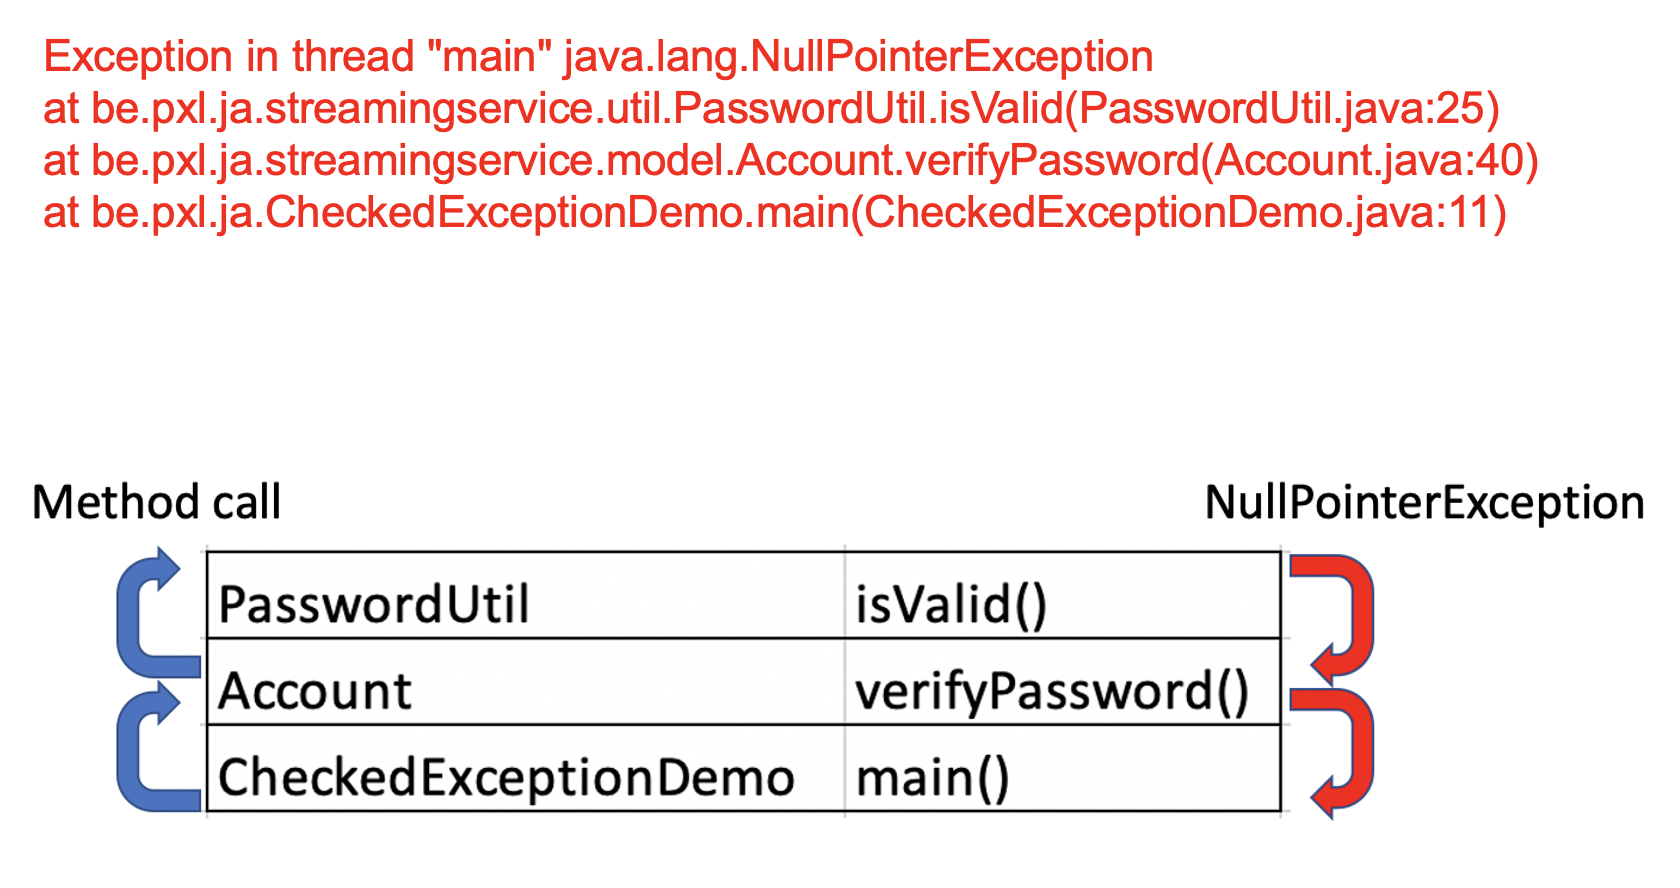
\includegraphics[width=\linewidth]{images/h2/exception_call_stack.png}
\caption{Method call stack}
\label{fig:method_call_stack}
\end{figure}

De NoSuchAlgorithmException wordt afgehandeld door null te geven als returnwaarde van de methode encodePassword.  Hierdoor wordt het probleem pas opgemerkt op het ogenblik dat we de methode isValid van de klasse PasswordUtil gebruiken. De informatie dat het foute algoritme werd meegegeven is momenteel volledig verloren gegaan. Daarom wordt altijd aangeraden om exceptions die zich voordoen in je programma bij te houden in logbestanden. Het gebruik van logbestanden valt buiten de scope van deze cursus. Als alternatief voor het loggen van exceptions zullen we in deze cursus de stacktrace van de exception tonen in de console.

\begin{lstlisting}
import java.math.BigInteger;
import java.security.MessageDigest;
import java.security.NoSuchAlgorithmException;

public class PasswordUtil {

	private static final String ALGORITHM = "MD4";

	public static String encodePassword(String password) {
		MessageDigest messageDigest = null;
		try {
			messageDigest = MessageDigest.getInstance(ALGORITHM);
		} catch (NoSuchAlgorithmException e) {
			e.printStackTrace();
			return null;
		}
		messageDigest.update(password.getBytes(), 0, password.length());
		return new BigInteger(1, messageDigest.digest()).toString(16);
	}

	public static boolean isValid(String providedPassword, String securedPassword) {
		return encodePassword(providedPassword).equals(securedPassword);
	}
}
\end{lstlisting}
 
Door de stacktrace te tonen in de console raken we geen cruciale informatie kwijt.

\begin{verbatim}
java.security.NoSuchAlgorithmException: MD4 MessageDigest not available
	at java.base/sun.security.jca.GetInstance.getInstance(GetInstance.java:159)
	at java.base/java.security.Security.getImpl(Security.java:700)
	at java.base/java.security.MessageDigest.getInstance(MessageDigest.java:177)
	at be.pxl.ja.streamingservice.util.PasswordUtil.encodePassword(PasswordUtil.java:15)
	at be.pxl.ja.streamingservice.model.Account.setPassword(Account.java:45)
	at be.pxl.ja.streamingservice.model.Account.<init>(Account.java:16)
	at be.pxl.ja.streamingservice.CheckedExceptionDemo.main(CheckedExceptionDemo.java:8)
java.security.NoSuchAlgorithmException: md4 MessageDigest not available
	at java.base/sun.security.jca.GetInstance.getInstance(GetInstance.java:159)
	at java.base/java.security.Security.getImpl(Security.java:700)
	at java.base/java.security.MessageDigest.getInstance(MessageDigest.java:177)
	at be.pxl.ja.streamingservice.util.PasswordUtil.encodePassword(PasswordUtil.java:15)
	at be.pxl.ja.streamingservice.util.PasswordUtil.isValid(PasswordUtil.java:25)
	at be.pxl.ja.streamingservice.model.Account.verifyPassword(Account.java:37)
	at be.pxl.ja.streamingservice.CheckedExceptionDemo.main(CheckedExceptionDemo.java:9)
Exception in thread "main" java.lang.NullPointerException
	at be.pxl.ja.streamingservice.util.PasswordUtil.isValid(PasswordUtil.java:25)
	at be.pxl.ja.streamingservice.model.Account.verifyPassword(Account.java:37)
	at be.pxl.ja.streamingservice.CheckedExceptionDemo.main(CheckedExceptionDemo.java:9)
\end{verbatim}

Opnieuw zie je het belang van unit testen. Een foute waarde voor het gekozen algoritme ga je al heel snel opmerken en herstellen als je unit testen schrijft voor de methoden encodePassword() en isValid().

In dit voorbeeld is het eigenlijk aangewezen om de exception niet af te handelen. Een alternatief is dat we de methode encodePassword() toelaten om de exception, als die zich voordoet, gewoon verder door te geven (gooien).
Hierdoor komt de exception dus terecht op de plaatsen waar je de methode encodePassword() gaat aanroepen en moet je op die plaatsen afhandeling voorzien. Je kan er dus voor kiezen om de checked exception NoSuchAlgorithmException helemaal mee te sleuren doorheen je applicatie tot aan de main()-methode.

\begin{lstlisting}
import java.math.BigInteger;
import java.security.MessageDigest;
import java.security.NoSuchAlgorithmException;

public class PasswordUtil {

	private static final String ALGORITHM = "MD5";

	public static String encodePassword(String password) throws NoSuchAlgorithmException {
		MessageDigest messageDigest = MessageDigest.getInstance(ALGORITHM);
		messageDigest.update(password.getBytes(), 0, password.length());
		return new BigInteger(1, messageDigest.digest()).toString(16);
	}

	public static boolean isValid(String providedPassword, String securedPassword) throws NoSuchAlgorithmException {
		return encodePassword(providedPassword).equals(securedPassword);
	}
}
\end{lstlisting}

\begin{lstlisting}
import java.security.NoSuchAlgorithmException;
import java.util.ArrayList;
import java.util.List;

public class Account {
	private String email;
	private String password;

	public Account(String email, String password) throws NoSuchAlgorithmException {
		this.email = email;
		setPassword(password);
	}

	public String getEmail() {
		return email;
	}

	public void setEmail(String email) {
		this.email = email;
	}

	public boolean verifyPassword(String password) throws NoSuchAlgorithmException {
		return PasswordUtil.isValid(password, this.password);
	}

	public void setPassword(String password) throws NoSuchAlgorithmException {
		this.password = PasswordUtil.encodePassword(password);
	}
}
\end{lstlisting}

\begin{lstlisting}
import be.pxl.ja.streamingservice.model.Account;
import java.security.NoSuchAlgorithmException;

public class CheckedExceptionDemo {

	public static void main(String[] args) throws NoSuchAlgorithmException {
		Account newAccount = new Account("daffy@duckstad.be", "daffy123!");
		System.out.println(newAccount.verifyPassword("daffy123"));
		System.out.println(newAccount.verifyPassword("daffy123!"));
	}
}
\end{lstlisting}

Je ziet dat nu bij de signatuur van verschillende methoden ``throws NoSuchAlgorithmException'' verschijnt.
Regelmatig verschijnen er artikels met titels als ``Checked exceptions: Java’s biggest mistake'' en ``Checked Exceptions are Evil'' om het gebruik van checked exceptions te ontmoedigen. 

Een laatste en nette oplossing is om de NoSuchAlgorithmException the \textbf{wrappen}  in een runtime exception bijv. een IllegalArgumentException.

\begin{lstlisting}
import java.math.BigInteger;
import java.security.MessageDigest;
import java.security.NoSuchAlgorithmException;

public class PasswordUtil {

	private static final String ALGORITHM = "MD4";

	public static String encodePassword(String password) {
		MessageDigest messageDigest = null;
		try {
			messageDigest = MessageDigest.getInstance(ALGORITHM);
		} catch (NoSuchAlgorithmException e) {
			throw new IllegalArgumentException(e);
		}
		messageDigest.update(password.getBytes(), 0, password.length());
		return new BigInteger(1, messageDigest.digest()).toString(16);
	}

	public static boolean isValid(String providedPassword, String securedPassword) {
		return encodePassword(providedPassword).equals(securedPassword);
	}
}
\end{lstlisting}

Bij het uitvoeren van de methode encodePassword() met een foutief algoritme krijg je dan een runtime exception.

\begin{verbatim}
Exception in thread "main" java.lang.IllegalArgumentException: java.security.NoSuchAlgorithmException: MD4 MessageDigest not available
	at be.pxl.ja.streamingservice.util.PasswordUtil.encodePassword(PasswordUtil.java:17)
	at be.pxl.ja.streamingservice.model.Account.setPassword(Account.java:48)
	at be.pxl.ja.streamingservice.model.Account.<init>(Account.java:18)
	at be.pxl.ja.CheckedExceptionDemo.main(CheckedExceptionDemo.java:10)
	at java.base/jdk.internal.reflect.NativeMethodAccessorImpl.invoke0(Native Method)
	at java.base/jdk.internal.reflect.NativeMethodAccessorImpl.invoke(NativeMethodAccessorImpl.java:62)
	at java.base/jdk.internal.reflect.DelegatingMethodAccessorImpl.invoke(DelegatingMethodAccessorImpl.java:43)
	at java.base/java.lang.reflect.Method.invoke(Method.java:564)
	at com.intellij.rt.execution.application.AppMainV2.main(AppMainV2.java:131)
Caused by: java.security.NoSuchAlgorithmException: MD4 MessageDigest not available
	at java.base/sun.security.jca.GetInstance.getInstance(GetInstance.java:159)
	at java.base/java.security.Security.getImpl(Security.java:700)
	at java.base/java.security.MessageDigest.getInstance(MessageDigest.java:177)
	at be.pxl.ja.streamingservice.util.PasswordUtil.encodePassword(PasswordUtil.java:15)
	... 8 more
\end{verbatim}

\section{Multi-catch blok en finally}

\begin{lstlisting}
import java.util.Scanner;

public class MultiCatchBlockDemo {

	public static void main(String[] args) {
		Scanner scanner = new Scanner(System.in);
		System.out.println("Kies een positie: ");
		int positie = scanner.nextInt();
		System.out.println("Kies een deler: ");
		int deler = scanner.nextInt();
		try {
			int getallen[] = new int[10];
			getallen[positie] = 30 / deler;
		} catch (ArrayIndexOutOfBoundsException e) {
			System.out.println("Je moet een positie kiezen tussen 0 en 9.");
		} catch (Exception e) {
			System.out.println(e.getMessage());
		} finally {
			System.out.println("Je koos positie " + positie);
		}
		System.out.println("Start je het programma nog een keer.");
	}
}
\end{lstlisting}

Een try-blok kan gevolgd worden door \'e\'en of meerder catch-blokken.
Wanneer een exception optreedt zal bij het eerste catch-blok gestart worden. Indien onze exception een instantie is van de opgevangen exception  (instanceof) dan zal dat catch-blok uitgevoerd worden en worden de volgende catch-blokken niet meer bekeken. Indien de exception geen instantie is van de opgevangen exception dan wordt er verder gekeken naar de volgende catch-blokken tot een overeenkomstig catch-blok worden gevonden. Indien er geen catch-blok wordt gevonden zal de runtime-exception doorstromen naar de aanroepende methode.

De volgorde van de catch-blokken is van belang. ArrayIndexOutOfBoundsException is een subklasse van Exception. Als we eerst een catch-blok aanmaken voor de superklasse en pas daarna een catch-blok voor de subklasse zou het tweede catch-blok ``onbereikbaar'' zijn. Het eerste catch-blok gaat de exception reeds kunnen afhandelen. Code die onbereikbaar is (unreachable code) wordt opgemerkt door de compiler wat resulteert in een compileerfout van je code.

\begin{oefening}
Wissel beide catch-blokken eens van plaats in bovenstaande code.
\end{oefening}

Het finally-blok tenslotte is een codeblok dat altijd wordt uitgevoerd: of er nu een exception optreedt of niet. Zelfs als er een exception optreedt en die niet kan worden afgehandeld door een catch-blok, zal toch het finally-blok uitgevoerd worden.

\begin{oefening}
Test de werking van het finally-blok eens uit met bovenstaand programma MultiCatchBlockDemo. Verwijder het tweede catch-blok eens en veroorzaak een deling door 0. Wat gebeurt er?
\end{oefening}

Indien je dezelfde code hebt om verschillende exceptions af te handelen, mag je exceptions combineren in een catch-block. Zo zal het catch-blok in onderstaand voorbeeld zowel ArrayIndexOutOfBoundsExceptions als ArithmeticExceptions afhandelen.

\begin{lstlisting}
public class MultipleCatches {

	public static void main(String[] args) {
		Scanner scanner = new Scanner(System.in);
		System.out.println("Kies een positie: ");
		int positie = scanner.nextInt();
		System.out.println("Kies een deler: ");
		int deler = scanner.nextInt();
		try {
			int getallen[] = new int[10];
			getallen[positie] = 30 / deler;
		} catch (ArrayIndexOutOfBoundsException | ArithmeticException e) {
			System.out.println(e.getMessage());
		}
		System.out.println("Start je het programma nog een keer.");
	}
}
\end{lstlisting}

\section{Zelf exceptions opgooien}
We willen gaan controleren dat de gebruikers van onze streaming service enkel geldige kredietkaartnummers invullen. Daarom maken we een aparte klasse CreditCardNumber. We gaan ervoor zorgen dat objecten van de klasse CreditCardNumber nooit ongeldige gegevens bevatten. Wanneer je een object van de klasse CreditCardNumber probeert aan te maken met ongeldige gegevens zal er een IllegalArgumentException gegooid worden.

We laten 2 types van kredietkaarten toe: VISA en MASTERCARD. Kaartnummers van VISA-kaarten starten altijd met het nummer 5, kaartnummers van MASTERCARD-kaarten starten altijd met 4.
Verder wordt ook gecontroleerd dat de kaartnummers bestaan uit 16 cijfers. Bestudeer de klasse CreditCardNumber.

\begin{lstlisting}
public class CreditCardNumber {
	private static final int LENGTH = 16;
	private static final int CVC_LENGTH = 3;

	private CreditCardType creditCardType;
	private String number;
	private String cvc;

	public CreditCardNumber(String number, String cvc) {
		if (!isNumeric(number) || number.length() != LENGTH) {
			throw new IllegalArgumentException("A card number must have " + LENGTH + " digits.");
		}
		creditCardType = getCreditCardType(number);
		if (creditCardType == null) {
			throw new IllegalArgumentException("This is not a valid credit card.");
		}
	}

	private boolean isNumeric(String text) {
		if (text == null || text.length() == 0) {
			return false;
		}
		try {
			Long.parseLong(text);
			return true;
		} catch (NumberFormatException e) {
			return false;
		}
	}

	private CreditCardType getCreditCardType(String number) {
		for (CreditCardType cardType : CreditCardType.values()) {
			if (cardType.getFirstNumber() == Integer.parseInt(number.substring(0, 1))) {
				return cardType;
			}
		}
		return null;
	}
}
\end{lstlisting} 

Natuurlijk gaan we de constructor van onze nieuwe klasse CreditCardNumber ook grondig testen.  Wanneer we dus foutieve waarden meegeven aan de constructor gaan we moeten verifi\"eren dat de IllegalArgumentException wordt opgegooid.

Hier is alvast een eenvoudig voorbeeld om te tonen hoe de methode assertThrows van de klasse Assertions in junit werkt.

\begin{lstlisting}
@Test
void testExpectedException() {
  Assertions.assertThrows(NumberFormatException.class, () -> {
    Integer.parseInt("One");
  });
}
\end{lstlisting}

De assertThrows() verwacht dat een NumberFormatException zal worden opgegooid. Omdat de string ``One'' een ongeldige waarde is zal de NumberFormatException ook effectief gegooid worden en zal de test dus slagen.

Nu zie je een aantal testen om onze constructor van de klasse CreditCardNumber te testen. Bestudeer de testen grondig.


\begin{lstlisting}
import org.junit.jupiter.api.Test;

import static org.junit.jupiter.api.Assertions.assertEquals;
import static org.junit.jupiter.api.Assertions.assertThrows;

public class CreditCardNumberTest {

	@Test
	public void validVisaCard() {
		CreditCardNumber creditCardNumber = new CreditCardNumber("4321876532147654", "123");

		assertEquals(CreditCardType.VISA, creditCardNumber.getType());
		assertEquals("123", creditCardNumber.getCvc());
		assertEquals("4321876532147654", creditCardNumber.getNumber());
	}

	@Test
	public void validVisaCardWithBlanks() {
		CreditCardNumber creditCardNumber = new CreditCardNumber("  43218 76532 1476 54  ", " 1 2 3 ");

		assertEquals(CreditCardType.VISA, creditCardNumber.getType());
		assertEquals("123", creditCardNumber.getCvc());
		assertEquals("4321876532147654", creditCardNumber.getNumber());
	}

	@Test
	public void validMasterCard() {
		CreditCardNumber creditCardNumber = new CreditCardNumber("5321876532147654", "123");

		assertEquals(CreditCardType.MASTERCARD, creditCardNumber.getType());
		assertEquals("123", creditCardNumber.getCvc());
		assertEquals("5321876532147654", creditCardNumber.getNumber());
	}

	@Test
	public void validMasterCardWithBlanks() {
		CreditCardNumber creditCardNumber = new CreditCardNumber("  53218 76532 1476 54  ", " 1 2 3 ");

		assertEquals(CreditCardType.MASTERCARD, creditCardNumber.getType());
		assertEquals("123", creditCardNumber.getCvc());
		assertEquals("5321876532147654", creditCardNumber.getNumber());
	}

	@Test
	public void throwsInvalidArgumentExceptionWhenNumberTooShort() {
		assertThrows(IllegalArgumentException.class, () -> {
			new CreditCardNumber("  53218 76532 1476  ", " 1 2 3 ");
		});
	}

	@Test
	public void throwsInvalidArgumentExceptionWhenNumberTooLong() {
		assertThrows(IllegalArgumentException.class, () -> {
			new CreditCardNumber("  53218 76532 1476 4445  ", " 1 2 3 ");
		});
	}

	@Test
	public void throwsInvalidArgumentExceptionWhenInvalidCardType() {
		assertThrows(IllegalArgumentException.class, () -> {
			new CreditCardNumber("7321876532147654", "123");
		});
	}
}
\end{lstlisting}

\begin{oefening}
Voeg in de constructor van de klasse CreditCardNumber een extra validatie toe voor de CVC (card validation code). De CVC is een getal bestaande uit 3 cijfers.
Pas je unit testen aan. Waarschijnlijk moet je extra unit testen toevoegen om de constructor van de klasse CreditCardNumber te testen.
\end{oefening}


\section{Zelf exception-klassen schrijven}

In de klasse CreditCardNumber hebben we gebruikgemaakt van een bestaande exception uit de JDK. We kunnen ook onze eigen Exception-klassen voorzien.

De klasse PaymentInfo gaan we nu grondig aanpassen door o.a. gebruik te maken van de klasse CreditCardNumber. Daarnaast willen we ook de vervaldatum van de kredietkaart gaan controleren. We willen namelijk dat de kredietkaart nog minstens 1 maand geldig is op het ogenblik dat de betaalgegevens worden ingegeven. Indien de vervaldatum binnen de maand valt, gaan we een InvalidDateException opgooien.

Deze InvalidDateException-klasse bestaat niet in de JDK, dus gaan we hem zelf voorzien. Wanneer je een \textbf{checked exception} wil maken gebruik je de klasse Exception als superklasse van je nieuwe exception. Wanneer je een \textbf{unchecked exception} wil maken gebruik je de klasse RuntimeException als superklasse.

Hier is alvast onze nieuwe exception klasse InvalidDateException. Als je zelf een exception klasse aanmaakt kan je zelf beslissen welke parameters en extra eigenschappen je voorziet in de constructor. Regelmatig wordt ook de afspraak gehanteerd dat er pas een nieuwe exception klasse wordt toegevoegd, indien \'e\'en van de reeds bestaande exception klassen niet eenvoudig hergebruikt kan worden. In ons geval, gaan we de ongeldige datum willen tonen. Om het samenstellen van de foutboodschap te kunnen hergebruiken is het dus zinvol om een InvalidDateException te maken met o.a. de ongeldige datum (LocalDate) als parameter.

\begin{lstlisting}
public class InvalidDateException extends RuntimeException {

	public static final DateTimeFormatter FORMATTER = DateTimeFormatter.ofPattern("dd/MM/yyyy");

	public InvalidDateException(LocalDate incorrectDate, String type, String description) {
		super(FORMATTER.format(incorrectDate) + " is not a valid " + type + ". " + description);
	}
}
\end{lstlisting}

\begin{lstlisting}
import java.time.LocalDate;

public class PaymentInfo {

	private String firstName;
	private String lastName;
	private CreditCardNumber cardNumer;
	private LocalDate expirationDate;

	public String getFirstName() {
		return firstName;
	}

	public void setFirstName(String firstName) {
		this.firstName = firstName;
	}

	public String getLastName() {
		return lastName;
	}

	public void setLastName(String lastName) {
		this.lastName = lastName;
	}

	public void setCardNumer(CreditCardNumber cardNumer) {
		this.cardNumer = cardNumer;
	}

	public LocalDate getExpirationDate() {
		return expirationDate;
	}

	public void setExpirationDate(LocalDate expirationDate) {
		if (LocalDate.now().plusMonths(1).isAfter(expirationDate)) {
			throw new InvalidDateException(expirationDate, "expirationDate", "Must be valid for at least 1 month.");
		}
		this.expirationDate = expirationDate;
	}
}
\end{lstlisting}

We gaan deze  methode setExpirationDate nu ook grondig testen.

\begin{lstlisting}
import org.junit.jupiter.api.BeforeEach;
import org.junit.jupiter.api.Test;

import java.time.LocalDate;

import static org.junit.jupiter.api.Assertions.assertEquals;
import static org.junit.jupiter.api.Assertions.assertNotNull;
import static org.junit.jupiter.api.Assertions.assertThrows;

public class PaymentInfoSetExpirationDateTest {

	private PaymentInfo paymentInfo;

	@BeforeEach
	public void init() {
		paymentInfo = new PaymentInfo();
	}

	@Test
	public void throwsInvalidDateExceptionWhenExpirationDayWithinOneMonth() {
		LocalDate withinOneMonth = LocalDate.now().plusMonths(1).minusDays(1);
		assertThrows(InvalidDateException.class, () -> paymentInfo.setExpirationDate(withinOneMonth));
	}

	@Test
	public void expirationDayWithinExactlyOneMonthIsAllowed() {
		LocalDate exactlyOneMonth = LocalDate.now().plusMonths(1);
		paymentInfo.setExpirationDate(exactlyOneMonth);

		assertNotNull(paymentInfo.getExpirationDate());
		assertEquals(exactlyOneMonth, paymentInfo.getExpirationDate());
	}

	@Test
	public void expirationDayOverOneMonthIsAllowed() {
		LocalDate overOneMonth = LocalDate.now().plusMonths(1).plusDays(1);
		paymentInfo.setExpirationDate(overOneMonth);

		assertNotNull(paymentInfo.getExpirationDate());
		assertEquals(overOneMonth, paymentInfo.getExpirationDate());
	}

}
\end{lstlisting} 

\begin{oefening}
Schrijf ook een kort programma waarin je de InvalidDateException veroorzaakt. Vang de exception op en toon de foutboodschap (message)?
\end{oefening}




\chapter{Spring Validation}
    
\fcolorbox{black}[HTML]{E9F0E9}{\parbox{\textwidth}{%
\noindent \textbf{Learning goals}\\
De junior-collega
\begin{enumerate}[nolistsep]
\item kan gebruikmaken van Spring Validation
\item kan de correcte validatieregels gebruiken
\end{enumerate}}}

Wanneer Spring Boot een HTTP-verzoek ontvangt, is het belangrijk om de gegevens die met dat verzoek zijn meegestuurd te valideren.  Spring Boot heeft voorgedefinieerde validatoren waardoor het controleren van veelvoorkomende regels eenvoudig kan gebeuren.  Zo kan Spring Boot bijvoorbeeld heel eenvoudig controleren of een e-mailadres het juiste formaat heeft of een getal binnen een bepaald bereik valt,.
In Spring Boot is het uiteraard ook mogelijk om aangepaste of eigen validatieregels te programmeren.

Om Spring Validation te gebruiken voeg je een dependency toe aan het project.

\begin{lstlisting}
<dependency>
	<groupId>org.springframework.boot</groupId>
	<artifactId>spring-boot-starter-validation</artifactId>
</dependency>
\end{lstlisting}

Hier is een lijst van de meest gebruikte annotaties.

\begin{tabularx}{\textwidth}{|l|X|}
\hline
@NotNull & om aan te duiden dat een referentie niet null mag zijn. \\
@NotEmpty & om aan te duiden dat een list elementen moet bevatten. \\
@NotBlank & om aan te duiden dat een string niet leeg mag zijn. \\
@Min and @Max & om aan te duiden dat een numerieke waarde enkel geldig is als de waarde groter of kleiner is dan een gegeven waarde.\\
@Size &  om de lengte van een string te valideren. \\
@Email & om te controleren of een string een geldig e-mailadres bevat.\\
\hline
\end{tabularx}

\begin{lstlisting}[language=java, frame=single]
package be.pxl.demo.domain;

import com.fasterxml.jackson.annotation.JsonProperty;
import jakarta.validation.constraints.Min;
import jakarta.validation.constraints.NotBlank;
import jakarta.validation.constraints.NotNull;

public class Song {
	@NotBlank
	private String title;
	@NotBlank
	private String artist;
	@JsonProperty("duration_seconds")
	@Min(value = 1, message = "Must be greater than zero")
	private int durationSeconds;
	@NotNull
	private Genre genre;
	
	...
}
\end{lstlisting}

Wanneer Spring Boot een argument vindt dat is geannoteerd met @Valid,  wordt het automatisch gevalideerd.

\begin{lstlisting}
@RestController
@RequestMapping("/playlist/songs")
public class MusicPlaylistController {

	private static final Logger LOGGER = LoggerFactory.getLogger(MusicPlaylistController.class);
	private final MusicPlaylistService musicPlaylistService;

	@Autowired
	public MusicPlaylistController(MusicPlaylistService musicPlaylistService) {
		this.musicPlaylistService = musicPlaylistService;
	}

	@PostMapping
	public void addSong(@RequestBody @Valid Song song) {
		if (LOGGER.isInfoEnabled()) {
			LOGGER.info("Adding song [" + song.getTitle() + "]");
		}
		musicPlaylistService.addSong(song);
	}
   ...
}
\end{lstlisting}

Wanneer het argument niet voldoet aan de regels dan gooit Spring Boot een exception van de klasse MethodArgumentNotValidException.

Sinds Spring Boot versie 2.3 moet je de eigenschap server.error.include-message de waarde always geven om de foutboodschappen te kunnen zien in het response. Spring Boot verbergt namelijk het foutmelding in de respons om het lekken van gevoelige informatie te voorkomen. 

De foutmelding blijft ondanks in de instelling eerder cryptisch.  Stel dat ik de REST API gebruik om een lied toe te voegen met de volgende gegevens:

\begin{verbatim}
{
  "title": "",
  "artist": "Bruno Mars",
  "duration_seconds": -2,
  "genre": "OTHER"
}
\end{verbatim}

Dan krijg je het volgende respons.

\begin{verbatim}
{
	"timestamp": "2023-09-23T13:48:50.490+00:00",
	"status": 400,
	"error": "Bad Request",
	"message": "Validation failed for object='song'. Error count: 2",
	"path": "/playlist/songs"
}
\end{verbatim}

Meer gegevens krijg ik te zien als ik de eigenschap server.error.include-binding-errors=always toevoeg in application.properties. Voor bovenstaande RequestBody krijg je dan de volgende respons. Er wordt op dat ogenblik al veel interne informatie gelekt.

\begin{lstlisting}[language=json]
{
	"timestamp": "2023-09-23T13:52:38.028+00:00",
	"status": 400,
	"error": "Bad Request",
	"message": "Validation failed for object='song'. Error count: 2",
	"errors": [
		{
			"codes": [
				"Min.song.durationSeconds",
				"Min.durationSeconds",
				"Min.int",
				"Min"
			],
			"arguments": [
				{
					"codes": [
						"song.durationSeconds",
						"durationSeconds"
					],
					"arguments": null,
					"defaultMessage": "durationSeconds",
					"code": "durationSeconds"
				},
				10
			],
			"defaultMessage": "Invalid duration_seconds: must equal or exceed 10.",
			"objectName": "song",
			"field": "durationSeconds",
			"rejectedValue": -2,
			"bindingFailure": false,
			"code": "Min"
		},
		{
			"codes": [
				"NotBlank.song.title",
				"NotBlank.title",
				"NotBlank.java.lang.String",
				"NotBlank"
			],
			"arguments": [
				{
					"codes": [
						"song.title",
						"title"
					],
					"arguments": null,
					"defaultMessage": "title",
					"code": "title"
				}
			],
			"defaultMessage": "must not be blank",
			"objectName": "song",
			"field": "title",
			"rejectedValue": "",
			"bindingFailure": false,
			"code": "NotBlank"
		}
	],
	"path": "/playlist/songs"
}
\end{lstlisting}

De best practice om de MethodArgumentNotValidException af te handelen is door gebruik te maken van een exception handler.  Hierbij gebruiken we de annotaties @RestControllerAdvice en @ExceptionHandler. 

\begin{lstlisting}
package be.pxl.demo.config;

import org.springframework.http.HttpStatus;
import org.springframework.http.ResponseEntity;
import org.springframework.validation.ObjectError;
import org.springframework.web.bind.MethodArgumentNotValidException;
import org.springframework.web.bind.annotation.ExceptionHandler;
import org.springframework.web.bind.annotation.RestControllerAdvice;

import java.util.ArrayList;
import java.util.List;

@RestControllerAdvice
public class GlobalExceptionHandler {

	@ExceptionHandler(MethodArgumentNotValidException.class)
	public ResponseEntity<List<String>> handleValidationErrors(MethodArgumentNotValidException ex) {
		List<String> errors = new ArrayList<>();
		for (ObjectError error: ex.getBindingResult().getAllErrors()) {
			errors.add(error.getDefaultMessage());
		}
		return new ResponseEntity<>(errors, HttpStatus.BAD_REQUEST);
	}
}
\end{lstlisting}


De annotatie @RestControllerAdvice geeft aan dat deze klasse verantwoordelijk is voor het afhandelen van exceptions. Alle exception worden onderschept en indien er voor het type exception een handler is gedefinieerd, zal de bijhorende code worden uitgevoerd. 

In deze klasse is er enkel een methode voorzien voor het afhandelen van MethodArgumentNotValidExceptions. De methode herkennen we aan de annotatie @ExceptionHandler. Binnen de methode wordt een lijst met de foutmeldingen (errors) gegenereerd.

We passen de foutboodschap bij iedere validatie ook best aan.  Gebruik een duidelijke foutboodschap om de gebruiker duidelijk te maken welke gegevens hij moet doorgeven.
Als je een meertalige applicatie hebt, kan je best een key (zoals title.not.blank) doorgeven aan de frontend zodat de eigenlijk foutboodschap in de juiste taal getoond kan worden.


\begin{lstlisting}
	@NotBlank(message = "title.not.blank")
	private String title;
	@Min(value = 10, message = "Invalid duration_seconds: must be equal to or exceed 10.")
	private int durationSeconds;
\end{lstlisting}

Er wordt in het geval van een MethodArgumentNotValidException een HTTP status 400 met de volgende response body gegeven:
\begin{verbatim}
[
	"Invalid duration_seconds: must be equal to or exceed 10.",
	"title.not.blank",
	"Please provide artist name."
]
\end{verbatim}


\begin{oefening}
\textbf{Huizenjacht}

We voeren een aantal aanpassingen uit aan de klasse House.
\begin{itemize}
\item Voeg de volgende eigenschappen toe:
\begin{itemize}
\item area: oppervlakte van de woning in m\textsuperscript{2}
\item epcScore: waarde uit de opsomming EPCScore.
\end{itemize}
\item Verwijder de eigenschap price. De prijs is nu een berekende waarde. Vermenigvuldig de oppervlakte met de basisprijs per m\textsuperscript{2} en het percentage behorende bij de epc score.
De huidige basisprijs per m\textsuperscript{2} is 2356.75.  Voor huizen in Hasselt en Genk is er een meerprijs van 25\%. 
\item Voeg de methode markAsSold() toe.  Deze methode verandert de status van het huis van FOR\_SALE naar SOLD. Wanneer het huis al verkocht is gooi je een IllegalStateException op.
\item Pas vervolgens de POST en PUT requests aan. Bij het toevoegen van een huis zijn de volgende velden verplicht: code, name, area (minstens 50m\textsuperscript{2}), epc-score en city. 
Bij het updaten kan je enkel volgende velden aanpassen: name, area (minstens 50m\textsuperscript{2}), city en epc-score.
\item Voorzie een aangepast endpoint /houses/\{code\}/sold om een huis als verkocht te registreren.
\end{itemize}

Test alle endpoints grondig uit.

\begin{lstlisting}[language=java]
public enum EPCScore {
	A_PLUS(1.5),
	A(1.2),
	B(1),
	C(0.98),
	D(0.90),
	E(0.80),
	F(0.75);

	private double percentage;

	EPCScore(double percentage) {
		this.percentage = percentage;
	}

	public double getPercentage() {
		return percentage;
	}
}
\end{lstlisting}

\end{oefening}



\chapter{Unit testing}

\begin{summary}
De software die we ontwikkelen moet kwaliteitsvol zijn. Maar hoe kunnen we er nu voor zorgen dat we het aantal bugs in onze code zo laag mogelijk houden? E\'en van de strategie\"en om de kwaliteit van software te waarborgen is testen. Testen is een heel belangrijk aspect van softwareontwikkeling waar je ongetwijfeld nog heel veel over gaat leren. 

Als ontwikkelaar zorg je er altijd voor dat wanneer je de gevraagde functionalteit implementeert, je ook de nodige unit testen schrijft om de kwaliteit van je code te garanderen. Wanneer je unit testen schrijft, ga je alle methoden van je klasse testen. Een methode van een klasse is dus de ``unit'' die we gaan testen.
We gaan automatische testen schrijven. Dit betekent dat iedere keer dat de code wordt aangepast of uitgebreid de testen eenvoudig opnieuw kunnen worden uitgevoerd. Op die manier gaan de fouten die ontstaan tijdens de verdere ontwikkeling van de software snel ontdekt worden. Bedenk ook dat een fout, onduidelijkheid of bug die vroeg in het ontwikkelproces wordt aangepakt, maar een kleine impact heeft (ook financieel) ten opzicht van problemen die later pas opduiken.
\end{summary}

\section{JUnit}

In Java gaan we gebruikmaken van het framework JUnit5 om onze unit testen te schrijven.
JUnit5 is opgedeeld in 3 sub-projecten:  Jupiter, Vintage en Platform. JUnit Jupiter is het  sub-project dat wij gebruiken om onze testen te schrijven en voorziet de engine om deze testen uit te voeren.


https://education.launchcode.org/java-web-development/chapters/unit-testing/exercises.html

https://www.didattica.agentgroup.unimo.it/wiki/images/7/7b/Es01-JUnit.pdf

\section{Unit test voor een constructor}

We starten direct met een voorbeeld. In het vorige hoofdstuk hadden we de klasse Documentary aangemaakt. De klasse Documentary is een subklasse van Movie. Bij het aanmaken van een Documentary-object moet wel steeds als genre Genre.DOCUMENTARY ingevuld zijn. 

\begin{lstlisting}
package be.pxl.ja.opdracht1;

public class Documentary extends Movie {

	private String topic;

	public Documentary(String title, Rating rating) {
		super(title, rating);
		addGenre(Genre.DOCUMENTARY);
	}

	public String getTopic() {
		return topic;
	}

	public void setTopic(String topic) {
		this.topic = topic;
	}
}
\end{lstlisting}

We gaan dus de constructor van de klasse Documentary testen.

Onze testklassen gaan we niet mengen met onze eigenlijke programma. Ons hoofdprogramma en de klassen zitten meestal in een source-folder (src). Onze unit testen plaatsen we in een overeenkomstig package in de test-folder. Wanneer je een folder met de naam ``test'' hebt aangemaakt, markeer deze dan ook als test-folder.


\begin{lstlisting}
package be.pxl.ja.opdracht1;

import org.junit.jupiter.api.Test;

import static org.junit.jupiter.api.Assertions.assertEquals;

public class DocumentaryTest {

	private static final String TITLE = "Planet Earth";

	@Test
	public void documentaryConstructor() {
		// ACT
		Documentary documentary = new Documentary(TITLE, Rating.TEENS);

		// ASSERT
		assertEquals(TITLE, documentary.getTitle());
		assertEquals(Rating.TEENS, documentary.getRating());
		assertEquals(Genre.DOCUMENTARY, documentary.getGenre());
	}
}
\end{lstlisting}

\global\csname @topnum\endcsname 0

We hoeven enkel een @Test annotatie toe te voegen opdat een test herkend wordt en uitgevoerd kan worden. De eerste keer dat je de annotatie @Test toevoegt in het project zal deze nog niet gekend zijn. IntelliJ zal zelf voorstellen om JUnit te downloaden en toe te voegen aan het classpath. Zorg er wel voor dat je de juiste versie gebruikt. 


Wanneer je nu de unit test DocumentaryTest uitvoert kunnen er 3 mogelijke scenario's plaatsvinden. Ofwel slaagt de test, ofwel faalt \'e\'en van de beweringen (asserts) ofwel loopt er iets onverwachts fout. In het eerste geval krijgt je test een groene kleurcode, in het tweede scenario een oranje en in het laatste scenario een rode.

\begin{figure}[H]
  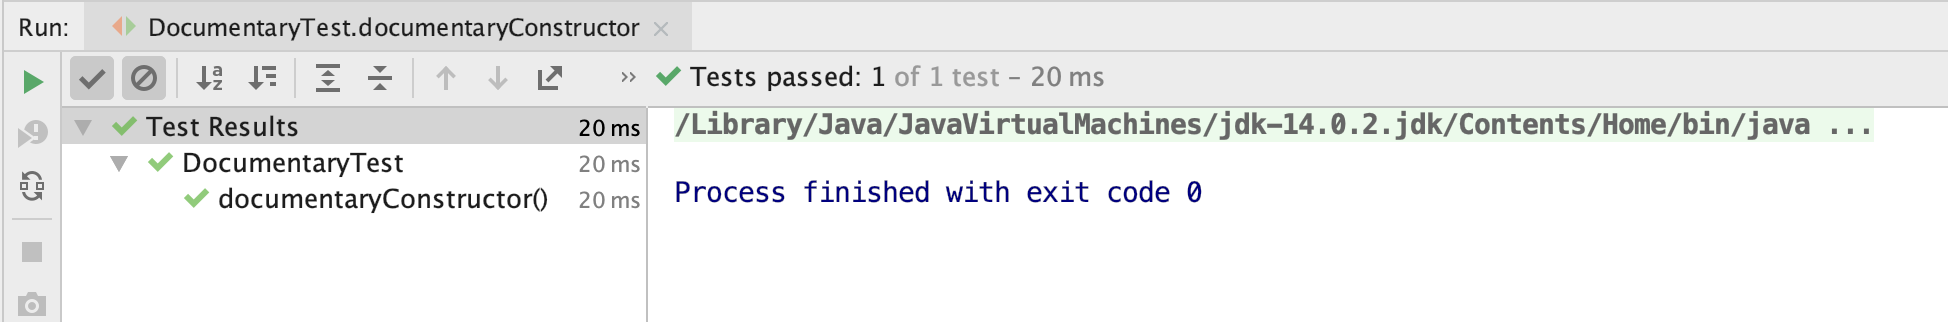
\includegraphics[width=\linewidth]{images/chapter-junit/junit_test_passed.png}
  \caption{Geslaagde JUnit5 test}
  \label{fig:test_passed}
\end{figure}

\begin{figure}[H]
  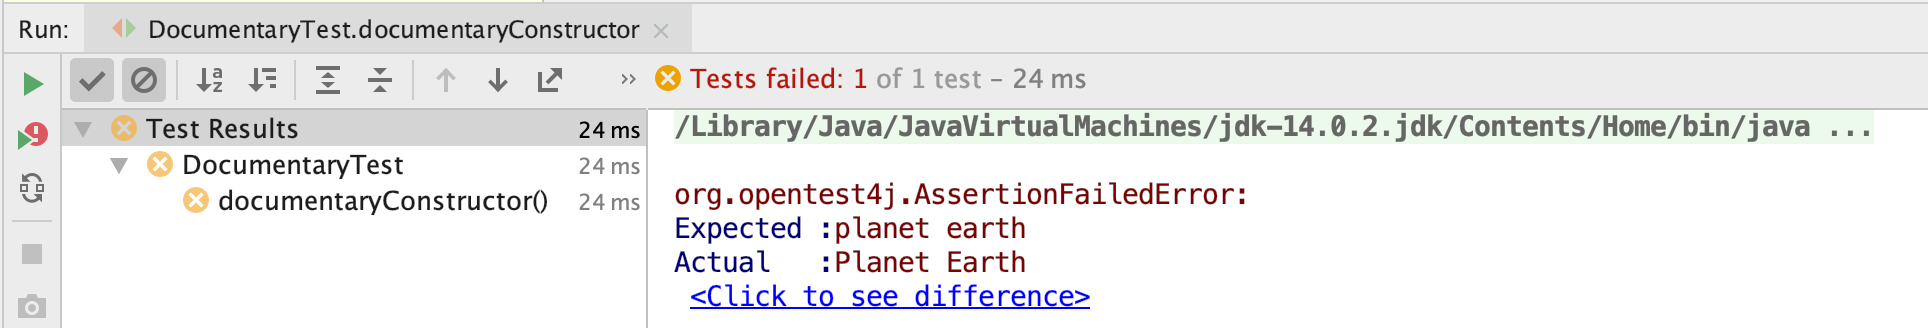
\includegraphics[width=\linewidth]{images/chapter-junit/junit_test_failed.png}
  \caption{Gefaalde JUnit5 test}
  \label{fig:test_failed}
\end{figure}



De methode van de Nederlandse weeramateurs is simpel. Het weercijfer tussen 0 en 10 wordt bepaald uit het weer overdag, tussen 7 en 19 uur. Een droge dag met nauwelijks bewolking of mist en weinig wind krijgt een 10. Afhankelijk van de hoeveelheid wolken vermindert dit met 1 tot 3 punten. Is het mistig dan kost dat, afhankelijk van de duur 1 of 2 punten. Voor de regen telt het aantal uurvakken met neerslag, dus ook alleen de duur. Zijn er tussen 7 en 19 uur twee uurvakken met regen dan kost dat 1 punt. Maar regent het in 11 of 12 uurvakken dan kost dat 4 punten.

Een zwakke wind kost geen punten, maar een matige wind van windkracht 3 gedurende minstens 3 uur kost 1 punt. De temperatuur speelt geen rol, zodat het weercijfer objectief is en ook koude, mooie dagen gunstig scoren. Langdurige regen overdag en veel wind leveren altijd een lage score.

\section{Unit test voor een setter}

Onze test zal steeds opgebouwd worden volgens het 3A patroon: Arrange, Act en Assert.
In iedere test herken je steeds deze 3 bouwstenen. 

Het ``arrange''-gedeelte is waar het object dat getest moet worden en alle andere objecten - die nodig zijn om de test goed uit te voeren - worden aangemaakt. 
Het ``act''-gedeelte is waar we de methode die we willen testen aanroepen. Als de methode een returnwaarde heeft ken je dit toe aan een variabele.

Het ``assert''-gedeelte geeft je de mogelijkheid om beweringen over het resultaat te verifi\"eren.

Hier is nog eens de klasse Movie.

\begin{lstlisting}
import java.time.LocalDate;

public class Movie extends Content implements Playable {
	private String director;
	private LocalDate releaseDate;
	private int duration;

	public Movie(String title, Rating rating) {
		super(title, rating);
	}

	public String getDirector() {
		return director;
	}

	public void setDirector(String director) {
		this.director = director;
	}

	public LocalDate getReleaseDate() {
		return releaseDate;
	}

	public void setReleaseDate(LocalDate releaseDate) {
		this.releaseDate = releaseDate;
	}

	public int getDuration() {
		return duration;
	}

	@Override
	public void play() {
		System.out.println("Playing " + this);
	}

	@Override
	public void pause() {
		System.out.println("Pausing " + this);
	}

	public boolean isLongPlayingTime() {
		return duration > LONG_PLAYING_TIME;
	}

	public String getPlayingTime() {
		// TODO: implement this method correctly		
		return "2 u 30 min";
	}

	@Override
	public String toString() {
		StringBuilder builder = new StringBuilder(super.toString());
		if (releaseDate != null) {
			builder.append(" (").append(releaseDate.getYear()).append(")");
		}
		return builder.toString();
	}
}
\end{lstlisting}

\global\csname @topnum\endcsname 0

Bekijk de methode void setDuration(int duration) eens. We willen nooit een negatief getal als waarde voor de eigenschap duration. Daarom zullen we de absolute waarde nemen van de parameter duration. Om deze setter te testen gaan we 2 testen voorzien. Een eerste test waar we een positieve waarde meegeven als argument en een tweede test waarbij we een negatieve waarde meegeven.

\begin{lstlisting}
import org.junit.jupiter.api.Test;

import static org.junit.jupiter.api.Assertions.assertEquals;

public class MovieSetDurationTest {

	@Test
	public void negativeDurationBecomesPositive() {
		// ARRANGE
		Movie movie = new Movie("Titanic", Rating.OLDER_KIDS);

		// ACT
		movie.setDuration(-125);

		// ASSERT
		assertEquals(125, movie.getDuration());
	}

	@Test
	public void positiveDurationStaysUnchanged() {
		// ARRANGE
		Movie movie = new Movie("Titanic", Rating.OLDER_KIDS);

		// ACT
		movie.setDuration(125);

		// ASSERT
		assertEquals(125, movie.getDuration());
	}
}
\end{lstlisting}

\clearpage

\section{Unit test voor een getter}

In de klasse Movie vind je ook de methode isLongPlayingTime() terug. Deze methode heeft een boolean als resultaat-type en geeft true indien de film langer dan 2 u 15 min duurt.

Hier is alvast 1 mogelijke unit test.

\begin{lstlisting}
import static org.junit.jupiter.api.Assertions.assertFalse;

public class MovieIsLongPlayingTimeTest {
	
	@Test
	public void movieWithDurationShorterThanLongPlayingTimeReturnsFalse() {
		
		Movie movie = new Movie("Titanic", Rating.TEENS);
		
		movie.setDuration(Movie.LONG_PLAYING_TIME - 1);
		
		assertFalse(movie.isLongPlayingTime());
	}
}
\end{lstlisting}

Bij de overige testen zullen in het Arrange gedeelte opnieuw een Movie-object moeten aanmaken. Omdat dit voor iedere test herzelfde is, hoeven we deze code niet te dupliceren. 
Met de annotatie @BeforeEach kunnen we een methode aanduiden die wordt uitgevoerd voor elke test.

Daarnaast merk je ook dat de klasse org.junit.jupiter.api.Assertions bijkomende static methoden heeft om de resultaten van de test te verifi\"eren. \textbf{assertFalse} en \textbf{assertTrue} zullen  slagen als de getestte waarde repectievelijk false of true is.

\begin{lstlisting}
import org.junit.jupiter.api.BeforeEach;
import org.junit.jupiter.api.Test;

import static org.junit.jupiter.api.Assertions.assertFalse;
import static org.junit.jupiter.api.Assertions.assertTrue;

public class MovieIsLongPlayingTimeTest {

	private Movie movie;

	@BeforeEach
	public void init() {
		movie = new Movie("Titanic", Rating.TEENS);
	}

	@Test
	public void movieWithDurationShorterThanLongPlayingTimeReturnsFalse() {

		movie.setDuration(Movie.LONG_PLAYING_TIME - 1);

		assertFalse(movie.isLongPlayingTime());
	}

	@Test
	public void movieWithDurationExactlyLongPlayingTimeReturnsFalse() {

		movie.setDuration(Movie.LONG_PLAYING_TIME);

		assertFalse(movie.isLongPlayingTime());
	}

	@Test
	public void movieWithDurationLongerThanLongPlayingTimeReturnsTrue() {

		movie.setDuration(Movie.LONG_PLAYING_TIME + 1);

		assertTrue(movie.isLongPlayingTime());
	}
}
\end{lstlisting}

We maken ook in de testen handig gebruik van de constante LONG\_PLAYING\_TIME. Door onze testen op deze manier te schrijven hoeven we de testen niet aan te passen als de waarde van LONG\_PLAYING\_TIME wordt aangepast. 

Hier is een overzicht van enkele handige static methoden uit de klasse org.junit.jupiter.api.Assertions. 

\begin{table}[h!]
\centering
\begin{tabularx}{\textwidth}{| l | X |}
 \hline
 Methode & Betekenis\\ 
 \hline\hline
assertEquals() & Evalueert de gelijkheid van 2 waarden. De test slaagt als beide
waarden gelijk (equal) zijn.\\
\hline
assertFalse() & Evaluatie van een booleaanse uitdrukking. De test slaagt indien
de uitdrukking false is.\\
\hline
assertTrue() & Evaluatie van een booleaanse uitdrukking. De test slaagt indien
de uitdrukking true is.\\
\hline
assertNotNull( ) & Vergelijkt een object referentie met null. De test slaagt indien de
object referentie niet null is.\\
\hline
assertSame( ) & Vergelijkt het geheugenadres van twee object referenties
(gebruik maken van == operator). De test slaagt indien beide
object referenties naar hetzelfde object verwijzen.\\
\hline
fail() & Zorgt ervoor dat de test zal falen.\\
 \hline
\end{tabularx}
\caption{Static methoden uit de klasse org.junit.jupiter.api.Assertions}
\label{table:assertions}
\end{table}

\begin{oefening}
Schrijf 2 unit testen voor de toString() methode van de klasse Movie. We verwachten dat deze methode de titel en het jaartal van de film teruggeeft (bijv. Titanic (1997)). Indien er geen releasedatum gekend is, wordt het jaartal achterwege gelaten.
\end{oefening}

\begin{oefening}
Schrijf unit testen voor de methode addGenre in de klasse Content. Let er ook op dat een  genre enkel wordt toegevoegd indien het niet eerder al werd toegevoegd. 
\end{oefening}

\begin{oefening}
Je ziet dat in bovenstaande klasse Movie de methode getPlayingTime() nog niet correct ge\"implementeerd is. Hier zijn alvast de unit testen. 

\begin{lstlisting}
import org.junit.jupiter.api.BeforeEach;
import org.junit.jupiter.api.Test;

import static org.junit.jupiter.api.Assertions.assertEquals;

public class MovieGetPlayingTimeTest {

	private Movie movie;

	@BeforeEach
	public void init() {
		movie = new Movie("Titanic", Rating.OLDER_KIDS);
	}

	@Test
	public void returnsQuestionmarkWhenDurationZero() {

		movie.setDuration(0);

		assertEquals("?", movie.getPlayingTime());
	}

	@Test
	public void returnsMinutesWhenDurationLessThan60() {

		movie.setDuration(59);

		assertEquals("59 min", movie.getPlayingTime());
	}

	@Test
	public void returnsHoursWhenDurationMultipleOf60() {

		movie.setDuration(120);

		assertEquals("2 h", movie.getPlayingTime());
	}

	@Test
	public void returnsHoursAndMinutesWhenDurationNotMultipleOf60() {

		movie.setDuration(135);

		assertEquals("2 h 15 min", movie.getPlayingTime());
	}
}
\end{lstlisting}

Bestudeer deze unit testen en implementeer vervolgens de methode. Test je implementatie uit! Wanneer alle testen slagen, bekijk dan je je code nog eens kritisch. Kan je nog verbeteringen aanbrengen in de code?
\end{oefening}

Je ziet dat je geen schrik moet hebben om achteraf je code te verbeteren. Omdat je beschikt over unit testen kan je rustig aan je code gaan sleutelen. Het proces om code te verbeteren en hierdoor de leesbaarheid en onderhoudbaarheid van de code te verhogen noemen we \textbf{refactoren}. 

\begin{remark}
  Meer weten over unit testing, kijk op pluralsight: \url{https://app.pluralsight.com/library/courses/junit-5-unit-testing-getting-started}
\end{remark}

\begin{oefening}
We gaan bij de domeinklassen van de streaming service nog enkele klassen en enums toevoegen. Deze klassen gaan we hergebruiken tijdens latere oefeningen. 

Je implementeert volgende enums en klassen in je oplossingen van opgave 1:
\begin{itemize}
\item CreditCardType
\item PaymentInfo
\item StreamingPlan
\item Profile
\item Account
\end{itemize}

\textbf{Enum CreditCardType}

CreditCardType is een eenvoudige enum-klasse met de waarden VISA en MASTERCARD.

\textbf{Klasse PaymentInfo}

Wanneer een gebruiker een account aanmaakt voor onze streaming service moet hij zijn betaalgegevens opgegeven. Deze gegevens houden we bij in een PaymentInfo-object.
Deze klasse bevat de volgende eigenschappen:

\begin{itemize}
\item cardNumber (String)
\item type (CreditCardType)
\item firstName (String)
\item lastName (String)
\item expirationDate (LocalDate)
\item securityCode (int)
\end{itemize}

Je hoeft enkel getters en setters te voorzien. Het valideren van cardNumber, securityCode en expirationDate houden we voor het volgende hoofdstuk wanneer we het hebben over foutafhandeling.

\textbf{Enum StreamingPlan}

Er zijn 3 producten waaruit gebruikers kunnen kiezen. Ieder product heeft een maximum aantal profielen per account en een prijs. 

Gebruikers met product BASIC kunnen maar 1 profiel aanmaken en betalen €7,99.
Gebruikers die kiezen voor STANDAARD kunnen 2 profielen aanmaken en betalen €11,99.
Tenslotte kunnen gebruikers met een PREMIUM account 4 profielen aanmaken. Zij betalen €15,99.

Maak een enum met de naam StreamingPlan met deze producten. Gebruik numberOfProfiles en price als eigenschappen voor deze enum-klasse. 

\textbf{Klasse Profile}

Afhankelijk van de StreamingPlan kunnen er dus profielen toegevoegd worden aan een account. Daarom implementeren we de klasse Profile. Voor iedere Profile-object willen we een naam (name) en een geboortedatum (dateOfBirth) weten. Deze laatste hebben we nodig om te beslissen of Content beschikbaar is of niet. 

Hiervoor voorzie je een methode \textit{boolean allowedToWatch(Content content)} in de klasse Profile. De methode geeft true als de content geschikt is voor het profiel (afhankelijk van de rating van de content en de geboortedatum van het profiel). 
De methode geeft false als de content niet geschikt is voor het profiel.
Zolang de geboortedatum niet is ingevuld is alle content niet geschikt voor het profiel.
Voeg de nodige unit testen toe om deze methode grondig te testen!

\textbf{Klasse Account}

En tenslotte voeg je de klasse Account toe. Een account heeft volgende eigenschappen:
\begin{itemize}
\item email
\item password
\item streamingPlan
\item \'e\'en of meerder profielen
\item paymentInfo
\end{itemize}

In de constructor van een Account wordt er direct 1 profiel aangemaakt met de naam "profile1" en geboortedatum 1/1/2000. Schrijf unit testen voor de constructor.

De methode getFirstProfile() geeft het eerste (en voorlopig ook enige) Profile-object terug als resultaat. 

De functionaliteit om profielen toe te voegen wordt in een volgend hoofdstuk toegevoegd.

\textbf{Optioneel: Sterkte van het paswoord}

Wanneer de gebruiker een account aanmaakt kiest hij een paswoord. We geven hem graag een indicatie of zijn gekozen paswoord voldoende sterk is.
Maak een hulpklasse \textbf{PasswordUtil}  met een static methode \textit{int calculateStrength(String password)}. 

Hier zijn de regels voor de berekening van de sterkte van een paswoord:
\begin{itemize}
\item Een paswoord met minder dan 6 karakters is zwak en geeft altijd een score van 0.
\item Een paswoord met een lengte tussen 6 en 10 geeft een score van 1.
\item Een paswoord met meer dan 10 karaketer geeft een score van 2.
\end{itemize}
Voor paswoorden met een lengte vanaf 6 karakters gelden de volgende bijkomende regels:
\begin{itemize}
\item Indien het paswoord minstens 1 cijfer bevat, wordt de score met 2 verhoogd.
\item Indien het paswoord minstens 1 kleine letter bevat, wordt de score met 2 verhoogd.
\item Indien het paswoord minstens 1 hoofdletter bevat, wordt de score met 2 verhoogd.
\item Indien het paswoord minstens 1 special karakter bevat, wordt de score met 2 verhoogd. Er is reeds een constante aanwezig in de klasse PasswordUtil die de speciale karakters bevat.
\end{itemize}
Implementeer deze regels en schrijf de nodige unit testen.
\end{oefening}

TODO klassendiagram



@Service
public class MusicPlaylistService {

    public String calculatePlaylistDuration(List<String> songDurations) {
        int totalSeconds = 0;

        for (String duration : songDurations) {
            String[] parts = duration.split(":");
            if (parts.length == 2) {
                int minutes = Integer.parseInt(parts[0]);
                int seconds = Integer.parseInt(parts[1]);
                totalSeconds += (minutes * 60) + seconds;
            }
        }

        int hours = totalSeconds / 3600;
        int remainingSeconds = totalSeconds % 3600;
        int minutes = remainingSeconds / 60;
        int seconds = remainingSeconds % 60;

        return String.format("%d:%02d:%02d", hours, minutes, seconds);
    }
}


\chapter{Lambda expressies en Streams}

\begin{summary}
De Stream API van Java biedt een elegante manier om collections te manipuleren. De belangrijkste interface uit de API is Stream$<$T$>$. Als Java ontwikkelaar gebruik je voornamelijk deze interface die alle implementatie-details verbergt. Bij het ontwerpen van de Stream API is, naast het aanbieden van een elegante en eenvoudige API, ook veel aandacht besteed aan performantie. 
\end{summary}

\section{Functionele interfaces}

\subsection{De interface StringConverter}

\begin{lstlisting}
@FunctionalInterface
public interface StringConverter {
	String convert(String original);
}
\end{lstlisting}

De interface StringConverter is een functionele interface. Een functionele interface is een interface met precies \'e\'en abstracte methode.  Het markeren van een functionele interface met de annotatie @FunctionalInterface is optioneel, maar het wordt wel aanbevolen om duidelijk te maken dat het de bedoeling is dat er maar \'e\'en abstracte methode in de interface staat.  De compiler waarschuwt dan als de interface niet langer een functionele interface is.

Een functionele interface mag standaardmethoden (default methoden) en statische methoden hebben.  Er mag echter maar \'e\'en abstracte methode zijn.

We maken nu de klasse UpperCaseConventer die de interface StringConverter implementeert. 
De convert methode zorgt ervoor dat de uppercase-versie van de originele string wordt aangemaakt en teruggegeven.

\begin{lstlisting}
public class UpperCaseConverter implements StringConverter{

	@Override
	public String convert(String original) {
		return original.toUpperCase();
	}
}
\end{lstlisting}


\begin{lstlisting}
public class Demo {

	public static void main(String[] args) {
		StringConverter upperCaseConverter = new UpperCaseConverter();
		System.out.println(upperCaseConverter.convert("LuchtHavenPerSOneeL"));
	}

}
\end{lstlisting}

Stel dat we nu ook een LowerCaseConverter,  een ReverseConverter, ...  willen aanmaken. Voor iedere functionaliteit die je nodig hebt, moet je een nieuwe klasse maken die de StringConverter-interface implementeert. 
Best wel wat werk,  zeker als je de klassen niet gaat hergebruiken. 
Gelukkig kan het eenvoudiger. Je kan namelijk anonieme innerklassen maken.

Je definieert en implementeert direct een instantie van een klasse zonder de klasse expliciet te benoemen. 

Hier gaan we:

\begin{lstlisting}
public class Demo {

	public static void main(String[] args) {
		StringConverter upperCaseConverter = new StringConverter() {
			@Override
			public String convert(String original) {
				return original.toUpperCase();
			}
		};
		StringConverter reverseConverter = new StringConverter() {
			@Override
			public String convert(String original) {
				StringBuilder temporary = new StringBuilder(original);
				return temporary.reverse().toString();
			}
		};
		System.out.println(upperCaseConverter.convert("LuchtHavenPerSOneeL"));
		System.out.println(reverseConverter.convert("LuchtHavenPerSOneeL"));
	}
}
\end{lstlisting}

Je kan voor iedere interface of abstracte klasse een anonieme innerklasse gebruiken.
Omdat we in dit geval te maken hebben met een functionele interface, kunnen we nog een stap verder gaan en een \textbf{lambda expressie} schrijven.

 Het proces om de anonieme innerklasse om te vormen naar een lambda expressie omvat het verwijderen van \'overhead\' en het vereenvoudigen van de syntax. 

\begin{lstlisting}
public class Demo {

	public static void main(String[] args) {
		StringConverter upperCaseConverter = (original) -> original.toUpperCase();
		StringConverter reverseConverter = (original) -> {
			StringBuilder temporary = new StringBuilder(original);
			return temporary.reverse().toString();
		};
		System.out.println(upperCaseConverter.convert("LuchtHavenPerSOneeL"));
		System.out.println(reverseConverter.convert("LuchtHavenPerSOneeL"));
	}
}
\end{lstlisting}

In de bovenstaande code hebben we de anonieme innerklassen vervangen door  lambda-expressies.  De lambda-expressies hebben de volgende onderdelen:

\begin{itemize}
\item de lijst met parameters - in dit geval (original), maar kan ook leeg zijn () of meerdere parameters bevatten.
\item -> scheidt de parameters van de expressie
\item expressie
\end{itemize}

We bereiken hetzelfde eindresultaat met aanzienlijk minder boilerplate code en een eenvoudigere leesbare syntax.


\begin{oefening}
Gegeven de volgende functionele interface:

\begin{lstlisting}
interface Calculator {
    int calculate(int n);
}
\end{lstlisting}

Maak een programma waarmee je 2 lambda expressies maakt met deze functionele interface. De eerste lambda expressie kan je gebruiken om de 2de-macht van het getal te bereken. De twee lambda expressie gebruik je om de 3de-macht van het getal te berekenen.
\end{oefening}

\subsection{Function$<$T, R$>$}

De generieke functionele interface Function voorziet een functie apply die een argument aanneemt en een resultaat produceert. Er zijn dus 2 verschillende generieke datatypes:
\begin{itemize}
\item T: het type van het argument 
\item R het type van het resultaat
\end{itemize}

\begin{lstlisting}
public class FunctionExample {
    public static void main(String[] args) {
        // Define a Function that converts a String to its length (an Integer)
        Function<String, Integer> stringLengthFunction = str -> str.length();

        // Apply the function to a String
        String inputString = "Hello, Function!";
        int length = stringLengthFunction.apply(inputString);

        System.out.println("Length of the string: " + length);
    }
}
\end{lstlisting}


\subsection{Consumer$<$T$>$}

De generieke functionele interface Consumer$<$T$>$ bevat een functie accept die \'e\'en argument aanneemt. De functie geeft geen resultaat terug. 

\begin{lstlisting}
ipublic class ConsumerExample {
    public static void main(String[] args) {
        List<String> names = new ArrayList<>();
        names.add("Alice");
        names.add("Bob");
        names add("Charlie");
        
        // Define a Consumer to print names
        Consumer<String> printName = name -> System.out.println("Name: " + name);
        
        // Iterate through the list and apply the Consumer using forEach
        names.forEach(printName);
    }
}
\end{lstlisting}

\begin{lstlisting}
public class ConsumerExample {
    public static void main(String[] args) {
        List<String> data = new ArrayList<>();
        data.add("Item 1");
        data.add("Item 2");
        data.add("Item 3");
        
        // Define a Consumer to process and modify elements
        Consumer<String> processItem = item -> {
            // Append " - Processed" to each item
            data.set(data.indexOf(item), item + " - Processed");
        };
        
        // Process and modify elements using the Consumer
        data.forEach(processItem);
        
        System.out.println("Processed Data: " + data);
    }
}
\end{lstlisting}


\subsection{Predicate$<$T$>$}

Predicate$<$T$>$ is een veelgebruikte functionele interface die een functie \textbf{test} voorziet met \'e\'en parameter met datatype T die een boolean-waarde (true of false) teruggeeft. Naast de abstracte methode test zijn er ook nog enkele default functies voorzien om Predicates te combineren met and, or en negate (not).

\begin{table}[h!]
\centering
\begin{tabularx}{\textwidth}{| l | X |}
 \hline
 Methode & Betekenis\\ 
 \hline
 boolean test(T t) &	It evaluates this predicate on the given argument.\\
 \hline
 default Predicate$<$T$>$ and(Predicate$<$? super T$>$ other)	& It returns a composed predicate that represents a short-circuiting logical AND of this predicate and another. When evaluating the composed predicate, if this predicate is false, then the other predicate is not evaluated.\\
\hline
 default Predicate$<$T$>$ or(Predicate$<$? super T$>$ other) &	It returns a composed predicate that represents a short-circuiting logical OR of this predicate and another. When evaluating the composed predicate, if this predicate is true, then the other predicate is not evaluated.\\
  \hline
 default Predicate$<$T$>$ negate()	& It returns a predicate that represents the logical negation of this predicate.\\
  \hline
\end{tabularx}
\end{table}


\begin{lstlisting}
public class PredicateExample {
    public static void main(String[] args) {
        List<String> names = new ArrayList<>();
        names.add("Alice");
        names.add("Bob");
        names.add("Charlie");
        names.add("Anna");

        Predicate<String> startsWithA = name -> name.startsWith("A");
        Predicate<String> endsWithe = name -> name.endsWith("e");

        Predicate<String> startsWithAAndEndsWithe = startsWithA.and(endsWithe);

        System.out.println(startsWithA.test("Alice"));
        System.out.println(startsWithAAndEndsWithe.test("Alice"));

        printElements(names, startsWithA);
    }
    
    public static void printElements(List<String> list, Predicate<String> predicate) {
        for (String item : list) {
            if (predicate.test(item)) {
                System.out.println(item);
            }
        }
    }
}
\end{lstlisting}


\section{External en internal iterators}

\begin{lstlisting}
package be.pxl.music.service;

import be.pxl.music.api.Genre;
import be.pxl.music.api.Song;
import org.springframework.stereotype.Service;

import java.util.ArrayList;
import java.util.List;

@Service
public class MusicPlaylistService {
	private List<Song> playlist = new ArrayList<>();

	... 
	
	public List<Song> getSongsByGenre(Genre genre) {
		List<Song> result = new ArrayList<>();
		for (Song song: playlist) {
			if (song.getGenre() == genre) {
				result.add(song);
			}
		}
		return result;
	}
}

\end{lstlisting}

Een stream maakt het mogelijk om op een functionele manier complexe bewerkingen uit te voeren op een verzameling.
We kunnen bovenstaande code schrijven met behulp van een stream. Onze external iterator verdwijnt en we krijgen een internal iterator in de plaats.

\begin{lstlisting}
public List<Song> getSongsByGenre(Genre genre) {
		return playlist.stream().filter(song -> song.getGenre() == genre).toList();
}
\end{lstlisting}

Een stream bestaat uit 3 delen: een (data) bron, intermediate operations (tussentijdse bewerkingen) en een terminal operation (eindbewerking). In ons voorbeeld is de playlist de bron, vervolgens hebben we een intermediate operation \textit{filter} en tenslotte een terminal operation \textit{toList()}.

\begin{figure}[H]
  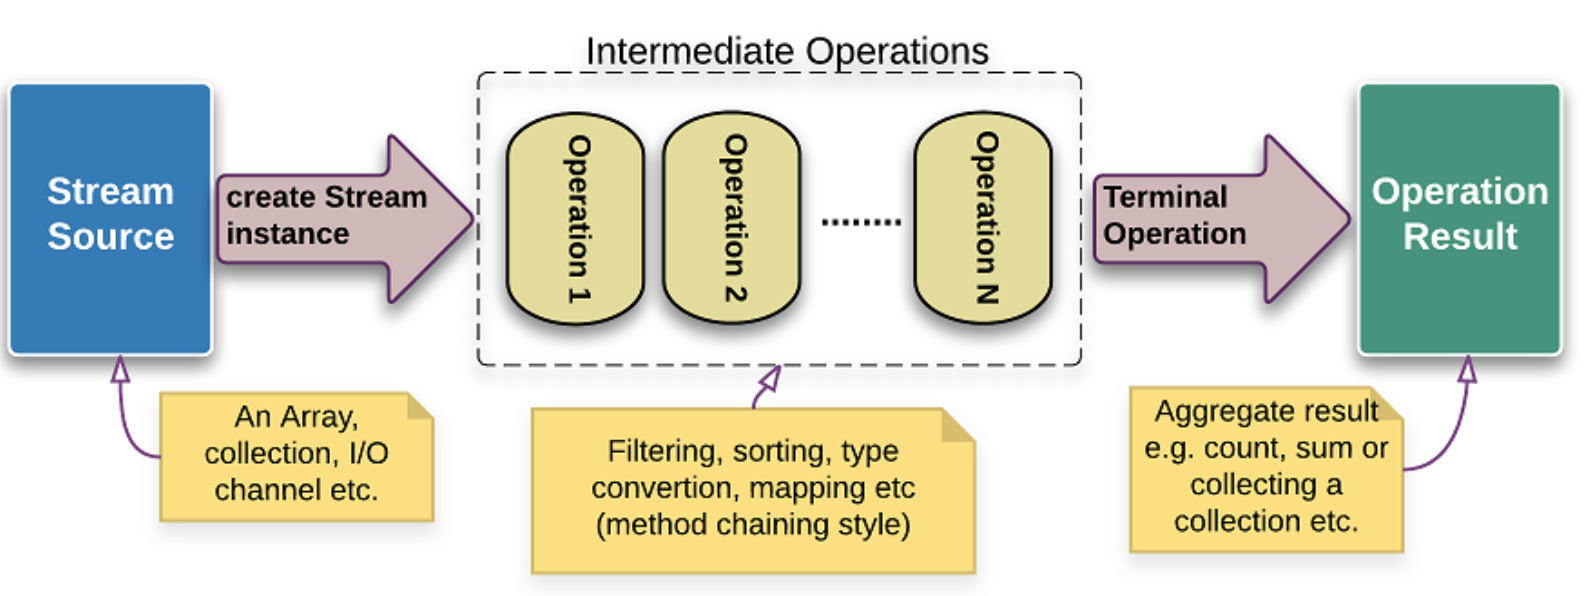
\includegraphics[width=\linewidth]{images/h6/stream_pipeline.png}
  \caption{Stream pipeline (logicbig.com)}
  \label{fig:stream_of}
\end{figure}


De intermediate operators verwerken de elementen van de stream \'e\'en voor \'e\'en. Alle intermediate operations zijn lui (lazy), ze worden enkel uitgevoerd als de stream wordt afgesloten door een terminal operation.

De internal iterator geniet meestal de voorkeur boven de external iterator.  Internal iterations kunnen korter geschreven worden en zijn daardoor ook makkelijker lees- en onderhoudbaar. Toch zijn er situaties, zoals wanneer je 2 verzamelingen gelijktijdig manipuleert, dat je kiest voor een external iterator.

\begin{figure}[H]
  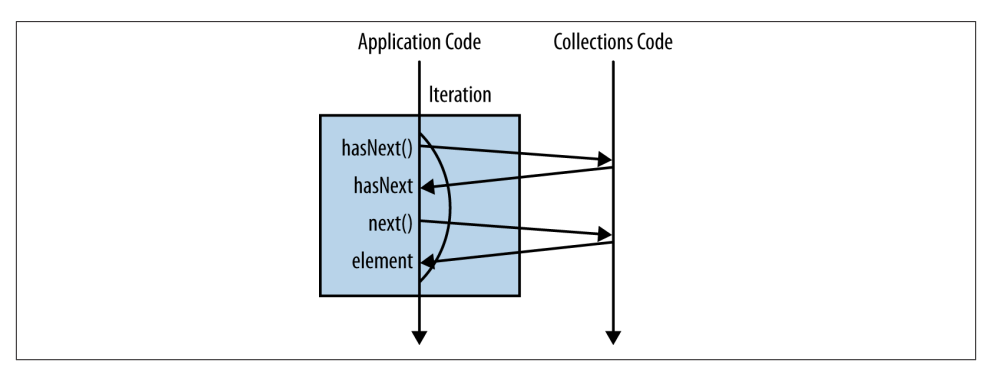
\includegraphics[width=\linewidth]{images/h6/external_iteration.png}
  \caption{External iteration}
  \label{fig:external_iteration}
\end{figure}

\begin{figure}[H]
  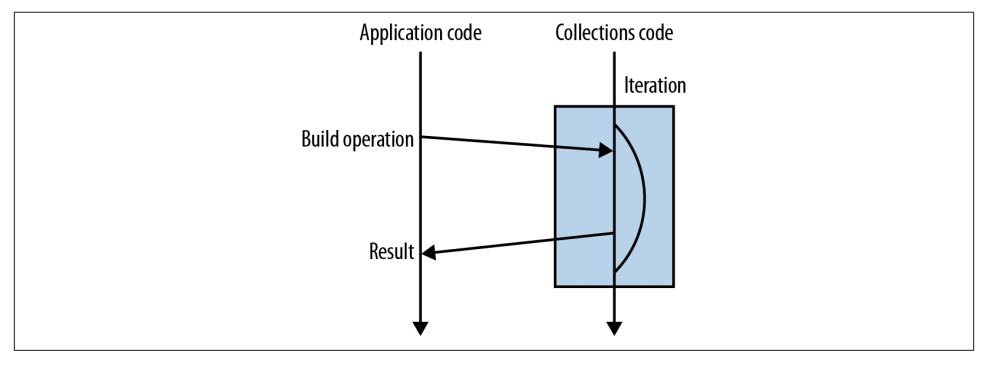
\includegraphics[width=\linewidth]{images/h6/internal_iteration.png}
  \caption{Internal iteration}
  \label{fig:internal_iteration}
\end{figure}



\section{Intermediate en terminal operations}

\subsection{Terminal operation .toList()}

\begin{lstlisting}
import java.util.List;
import java.util.stream.Collectors;
import java.util.stream.Stream;

public class DemoCollect {

	public static void main(String[] args) {

		List<String> theBeatles = 
				Stream.of("John Lennon", "Paul McCartney", "George Harrison", "Ringo Starr")
				.toList();
		System.out.println(theBeatles);
	}

}
\end{lstlisting}

Een stream is geen datastructuur of verzameling. Je moet een stream zien als een reeks objecten. E\'en van de manieren om zo'n reeks of stream te bouwen is met de static methode \textit{of} van de interface Stream.

\begin{figure}[H]
  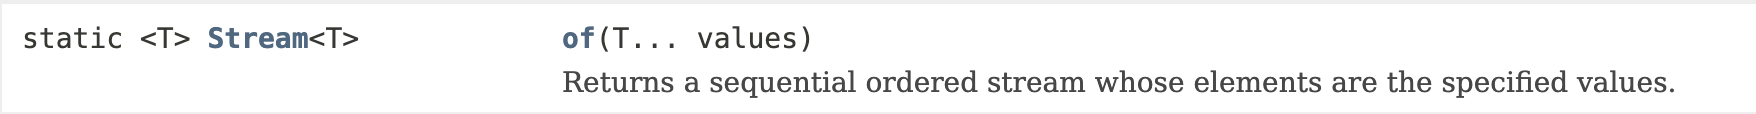
\includegraphics[width=\linewidth]{images/h6/stream_of.png}
  \caption{Static methode of() in de interface Stream}
  \label{fig:stream_of}
\end{figure}

Door gebruik te maken van de operation \textit{.toList()} kunnen we de objecten uit de stream verzamelen in een List.

\subsection{Intermediate operation .filter()}

Wanneer je bepaalde elementen uit een stream wil selecteren, gebruik je een filter. 

\begin{figure}[H]
  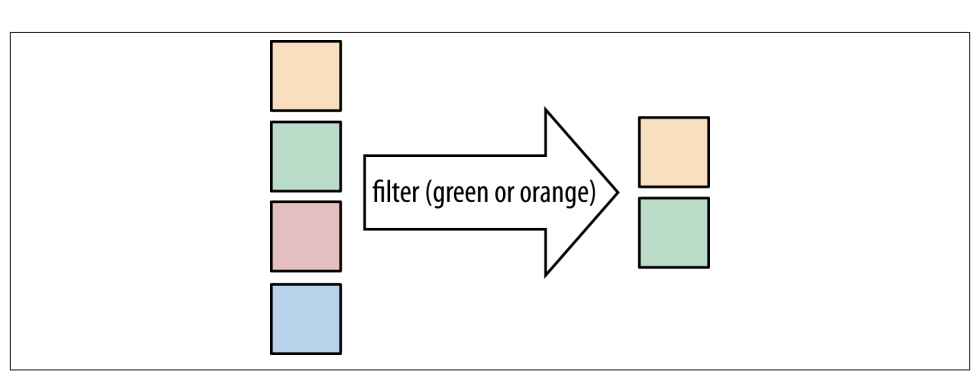
\includegraphics[width=\linewidth]{images/h6/illustration_filter.png}
  \caption{Filter operation}
  \label{fig:filter_operation}
\end{figure}

\begin{figure}[H]
  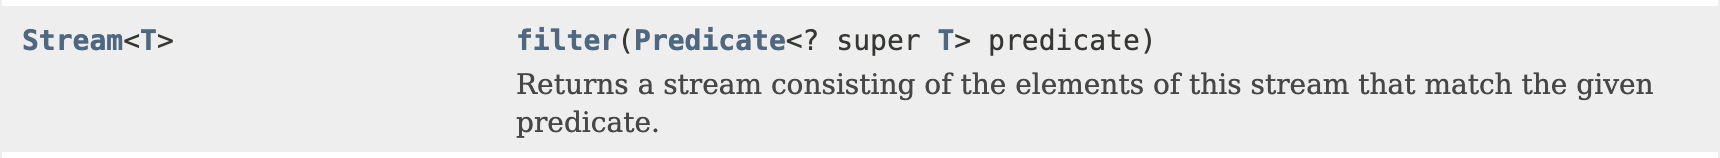
\includegraphics[width=\linewidth]{images/h6/stream_filter.png}
  \caption{Methode filter() in de interface Stream}
  \label{fig:stream_filters}
\end{figure}

Aan de hand van een Predicate wordt beslist welke elementen geselecteerd worden. 

In het onderstaande voorbeeld selecteren we de even getallen uit de verzameling numbers.

\begin{lstlisting}
List<Integer> numbers = Arrays.asList(1,2,3,4,5);

List<Integer> evenNumbers = numbers.stream()
				.filter(n -> n%2  == 0)
				.toList();
				
assertEquals(Arrays.asList(2,4), evenNumbers);
\end{lstlisting}

Nog een voorbeeld:

\begin{lstlisting}
List<String> animals = Stream.of("zebra", "dog", "dolphine")
				.filter(a -> a.contains("o"))
				.toList();

assertEquals(Arrays.asList("dog", "dolphine"), animals);
\end{lstlisting}

Alle String-objecten die een ``o'' bevatten mogen in de stream aanwezig blijven.

Merk op dat de functie filter() een intermediate operation is. De bewerking heeft als return-type Stream. We bouwen als het ware een pipeline. De filter()-operation is ook lazy en zal pas effectief uitgevoerd worden als er een terminal-operation aanwezig is.

Hier volgt nog een voorbeeld met een verzameling met objecten van een zelfgeschreven klasse Participant.

\begin{lstlisting}
public class Participant {
	private String name;
	private int points;

	public Participant(String name, int points) {
		this.name = name;
		this.points = points;
	}

	public int getPoints() {
		return points;
	}

	public String getName() {
		return name;
	}
}
\end{lstlisting}

\begin{lstlisting}
Participant john = new Participant("John P.", 15);
Participant sarah = new Participant("Sarah M.", 200);
Participant charles = new Participant("Charles B.", 150);
Participant mary = new Participant("Mary T.", 1);

List<Participant> participants = Arrays.asList(john, sarah, charles, mary);

List<Participant> over100Points = participants.stream()
     .filter(p -> p.getPoints() > 100)
     .toList();

assertEquals(Arrays.asList(sarah, charles), over100Points);
\end{lstlisting}

Je kan ook meerdere criteria gebruiken in een filter. Je kan in het Predicate de verschillende criteria samenvoegen via boolean operatoren.

\begin{lstlisting}
List<Participant> selection = participants.stream()
    .filter(p -> p.getPoints() > 100 && p.getName().startsWith("S"))
    .toList();
    
assertEquals(Collections.singletonList(sarah), selection);
\end{lstlisting}

Daarnaast kan je ook gebruikmaken van methodes als ``or'',  ``and'' en ``negate'' uit de interface Predicate.
		
\begin{lstlisting}
Predicate<Participant> over100Points = p -> p.getPoints() > 100;
Predicate<Participant> startingWithS = p -> p.getName().startsWith("S");

List<Participant> selection = participants.stream()
    .filter(over100Points.and(startingWithS))
    .toList();

assertEquals(Collections.singletonList(sarah), selection);
\end{lstlisting}

\subsection{Terminal operation .forEach()}

De methode .forEach() is een terminal operation en aanvaardt een implementatie van de functionele interface Consumer als parameter. Deze Consumer beschrijft een actie die met ieder element van de verzameling uitgevoerd zal worden.

\begin{figure}[H]
  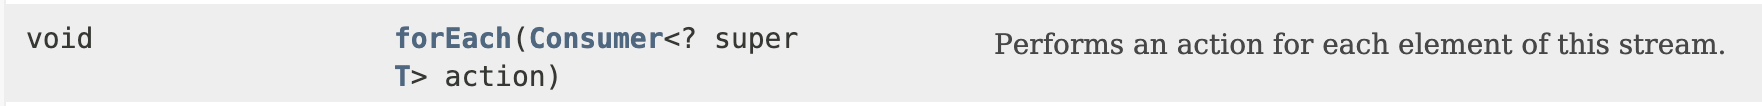
\includegraphics[width=\linewidth]{images/h6/stream_forEach.png}
  \caption{Methode forEach() in de interface Stream}
  \label{fig:stream_foreach}
\end{figure}

\begin{lstlisting}
public class DemoForEach {

	public static void main(String[] args) {
		Participant john = new Participant("John P.", 15);
		Participant sarah = new Participant("Sarah M.", 200);
		Participant charles = new Participant("Charles B.", 150);
		Participant mary = new Participant("Mary T.", 1);

		List<Participant> participants = Arrays.asList(john, sarah, charles, mary);

		participants.stream()
		    .filter(p -> p.getPoints() >= 200)
		    .forEach(System.out::println);

		System.out.println("* All participants *");

		participants.forEach(System.out::println);
	}
}
\end{lstlisting}

Iedere Collection biedt via de interface Iterable ook een forEach methode aan. Met beide forEach functies kan je hetzelfde resultaat bereiken.

\begin{lstlisting}
participants.forEach(System.out::println);
participants.stream().forEach(System.out::println);
\end{lstlisting}

Toch gaat in dit geval onze voorkeur uit naar de eerste optie. Omdat we hier itereren over alle elementen is de stream overbodig.


\subsection{Intermediate operation .map()}

Als je een functie hebt om objecten van \'e\'en datatype te transformeren naar een ander datatype, dan kan je met de bewerking .map(), deze functie loslaten op alle objecten van een stream. 

\begin{figure}[H]
  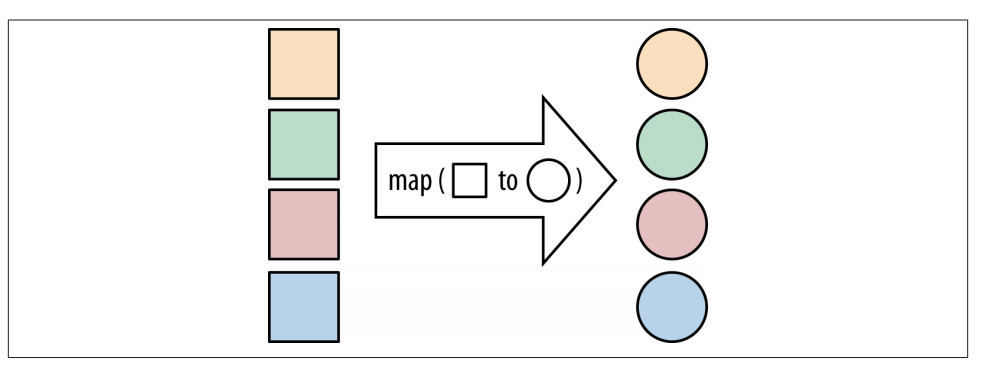
\includegraphics[width=\linewidth]{images/h6/illustration_map.png}
  \caption{Map operation}
  \label{fig:stream_foreach}
\end{figure}

\begin{figure}[H]
  
\includegraphics[width=\linewidth]{images/h6/stream_map.png}
  \caption{Methode map() in de interface Stream}
  \label{fig:stream_foreach}
\end{figure}

Map is een lazy operator. Zonder terminal operator zal de meegegeven functie niet uitgevoerd worden, en zal je dus ook geen resultaat krijgen. De functie die je meegeeft aan map is een implementatie van de generieke functionele interface Function$<$T,R$>$.

Hier volgen een twee voorbeelden. In het eerste voorbeeld wijzigt het datatype van de elementen van de stream niet. In het tweede voorbeeld wordt ieder String-object in de stream vervangen door een Integer-waarde.

\begin{lstlisting}
List<String> animals = Stream.of("zebra", "dog", "dolphine")
				.map(String::toUpperCase)
				.toList();

assertEquals(Arrays.asList("ZEBRA", "DOG", "DOLPHINE"), animals);
\end{lstlisting}

\begin{lstlisting}
List<Integer> lengths = Stream.of("zebra", "dog", "dolphine")
				.map(String::length)
				.toList();

assertEquals(Arrays.asList(5, 3, 8), lengths);
\end{lstlisting}

\subsection{Intermediate operation .sorted()}

Wanneer je de intermediate operation sorted() toevoegt aan een stream, worden de elementen in de stream gesorteerd. Zonder parameter zal sorted() de natuurlijke sortering gebruiken. Voor objecten van een zelfgeschreven klasse zorg je er dus voor dat de interface Comparable ge\"implementeerd wordt.

Het is ook mogelijk dat je aan de functie sorted() een parameter meegeeft waarmee je een andere volgorde kan afdwingen. In het tweede voorbeeld gebruiken we niet de natuurlijke (alfabetische) volgorde, maar worden de woorden van lang naar kort gesorteerd.


\begin{lstlisting}
List<String> sortedList = Stream.of("zebra", "dog", "dolphine")
				.sorted()
				.toList();

assertEquals(Arrays.asList("dog", "dolphine", "zebra"), sortedList);
\end{lstlisting}

\begin{lstlisting}
List<String> sortedList = Stream.of("zebra", "dog", "dolphine")
				.sorted((x, y) -> y.length() - x.length())
				.toList();
		
assertEquals(Arrays.asList("dolphine", "zebra", "dog"), sortedList);
\end{lstlisting}

\subsection{Intermediate operation .distinct()}

De operation .distinct() zorgt ervoor dat de elementen in de stream uniek zijn. Elementen die meermaals voorkomen worden verwijderd. Het is de implementatie van de equals() methode (en dus ook hashCode()) van een klasse die beslist of de elementen uniek zijn of niet.

\begin{lstlisting}
List<String> withoutDoubles = Stream.of("zebra", "dog", "zebra", "dolphine")
    .distinct()
    .toList();
    
assertEquals(3, withoutDoubles.size());
\end{lstlisting}

\subsection{Intermediate operation .limit()}

De operation .limit() heeft 1 parameter die het maximaal toegelaten elementen in de stream geeft.
De stream wordt dus als het ware afgekapt.

\begin{lstlisting}
List<String> animals = Stream.of("zebra", "dog", "elephant", "camel", "cat", "fish","dolphine")
    .limit(4)
    .toList();
assertEquals(4, animals.size());
\end{lstlisting}

Met de methode iterate kunnen we een oneindige stream maken. Dankzij de limit(5) worden slechts de eerste 5 nummers gegenereerd.

\begin{lstlisting}
List<Integer> numbers = Stream.iterate(1, n -> n + n)
    .limit(5)
    .toList();

assertEquals(Arrays.asList(1,2,4,8,16), numbers);
\end{lstlisting}


\subsection{Intermediate operation peek()}

De intermediate operation peek kan gebruikt worden om je pipeline te debuggen. Als je wilt controleren welke elementen er op een gegeven moment in de pipeline zitten, dan voeg je peek toe. Zolang je geen terminal operation hebt toegevoegd zal ook peek geen resultaat laten zien.

\begin{lstlisting}
Stream.of("one", "two", "three", "four")
  .filter(e -> e.length() > 3)
  .peek(e -> System.out.println("Filtered value: " + e))
  .map(String::toUpperCase)
  .peek(e -> System.out.println("Mapped value: " + e))
  .toList();
\end{lstlisting}

Je kan de operation peek() verder ook handig gebruiken om de elementen van je stream aan te passen.

\begin{lstlisting}
Stream<User> userStream = Stream.of(new User("Alice"), new User("Bob"), new User("Chuck"));
userStream.peek(u -> u.setName(u.getName().toLowerCase()))
  .forEach(System.out::println);
  \end{lstlisting}


\subsection{Terminal operation .count()}

\begin{lstlisting}
long over100Points = participants.stream().filter(p -> p.getPoints() > 100).count();

assertEquals(2, over100Points);
\end{lstlisting}
		
De terminal operation count gebruik je om het aantal elementen in de stream te tellen.
Indien je geen gebruik maakt van intermediate operations gebruik je de methode size() van je collection om het aantal elementen te achterhalen.

\begin{lstlisting}
System.out.println("Number of participants: " + participants.size());
\end{lstlisting}
		
\section{Intstream, LongStream en DoubleStream}
	
Er zijn ook een aantal afgeleide interfaces van de interface Stream. Deze bieden extra functionaliteit aan. Zo hebben we bijvoorbeeld de interface IntStream, die speciaal ontworpen is voor streams met gehele getallen. Deze stream bevat elementen met datatype \textit{int}. Naast IntStream hebben we ook de interfaces DoubleStream en LongStream. Al deze interfaces bevatten de methoden sum(), min(), max() en average(). 

\subsection{sum()}

Met de operation sum kan je eenvoudig de som berekenen van alle elementen in je stream.

\begin{lstlisting}
long totalPoints = participants.stream().mapToInt(Participant::getPoints).sum();

assertEquals(366, totalPoints);
\end{lstlisting}
		

\subsection{range() en rangeClosed()}
		
De static methoden range() en rangeClosed() zijn beschikbaar in de interfaces java.util.stream.IntStream en java.util.stream.LongStream. Je kan ze gebruiken om een stream te cre\"eren met gehele getallen vanaf een init\"ele waarde tot een stop waarde.
\begin{figure}[H]
  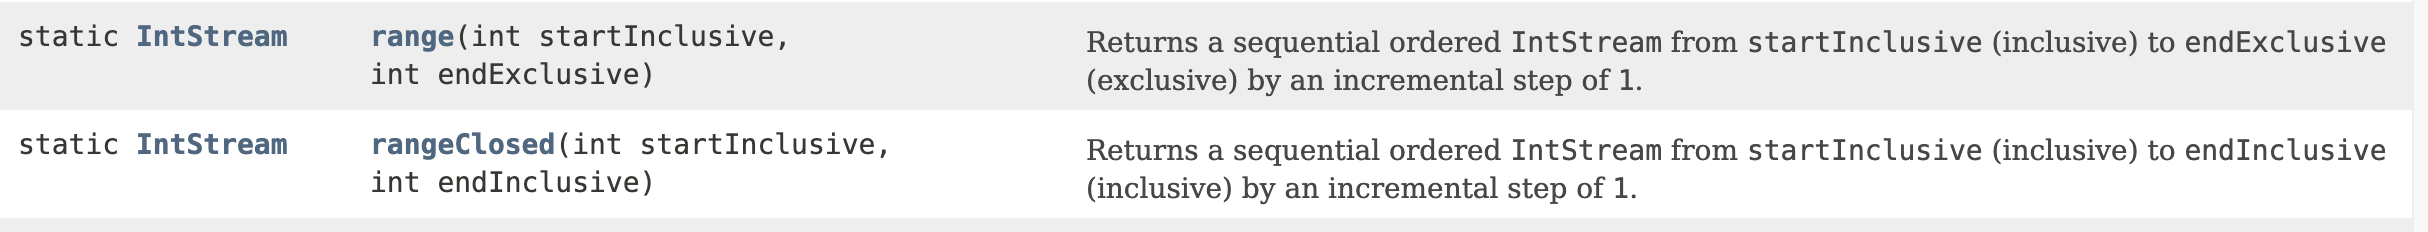
\includegraphics[width=\linewidth]{images/h6/intstream_range.png}
  \caption{Aanmaken van IntStream met range() of rangeClosed()}
  \label{fig:stream_foreach}
\end{figure}

\begin{lstlisting}
long count = IntStream.rangeClosed(10, 20).count();

assertEquals(11, count);
\end{lstlisting}

\subsection{min(), max() en average()}

\begin{figure}[H]
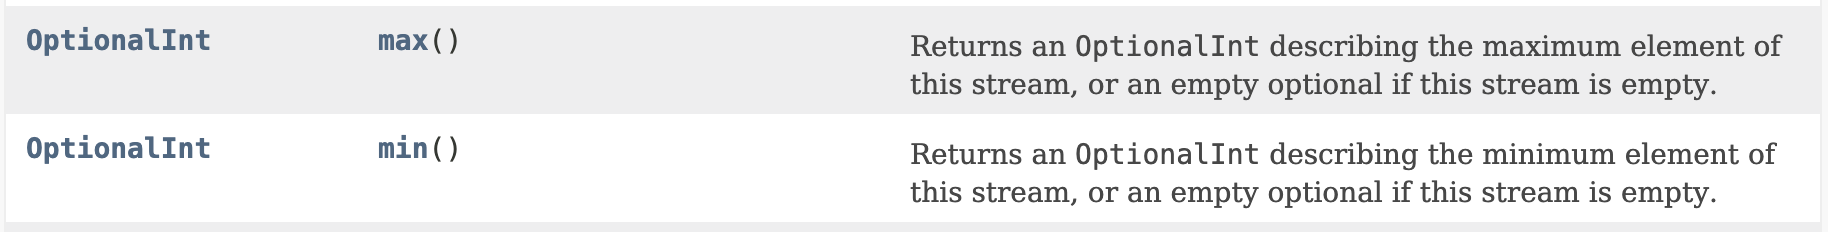
\includegraphics[width=\linewidth]{images/h6/intstream_max_min.png}
\caption{min() en max() uit de interface IntStream}
\label{fig:instream_min_max}
\end{figure}

\begin{figure}[H]

\includegraphics[width=\linewidth]{images/h6/intstream_average.png}
\caption{average() uit de interface IntStream}
\label{fig:instream_average}
\end{figure}

Merk op dat de methoden max() en min() een object van de klasse OptionalInt als return-type hebben. De methode average() heeft OptionalDouble als return-type. 

\begin{oefening}
Zoek de klasse OptionalInt en OptionalDouble op in de Java documentatie.
\end{oefening}

In de documentatie vind je terug dat dit een container-object is dat een int- of double-waarde kan bevatten. Indien we namelijk een lege stream hebben, dan bestaat er immers geen minimum, maximum of gemiddelde. In plaats van bijvoorbeeld een exception op te gooien wanneer we max() oproepen voor een lege IntStream, is er gekozen om steeds een OptionalInt als resultaat te geven. Bij een lege IntStream bevat het OptionalIInt-object geen waarde en \textit{isPresent()} geeft false als resultaat. Indien er wel een maximum berekend kan worden geeft \textit{isPresent()} true. De berekende waarde kan je bekomen via de methode \textit{getAsInt()}.

\begin{lstlisting}
Random random = new Random();
List<Integer> randomNumbers = random.ints(15, 0, 100).boxed().toList();
int max = randomNumbers.stream().mapToInt(x -> x).max().getAsInt();
int min = randomNumbers.stream().mapToInt(x -> x).min().getAsInt();
double average = randomNumbers.stream().mapToInt(x -> x).average().getAsDouble();
assertTrue(min <= average);
assertTrue(max >= average);

IntSummaryStatistics intSummaryStatistics = random.ints(15, 0, 100).summaryStatistics();
assertTrue(intSummaryStatistics.getMax() >= intSummaryStatistics.getMin());
\end{lstlisting}


\section{Method reference}

Method references zijn een speciaal type lambda expressies. Ze worden gebruikt om lambda expressies te vereenvoudigen door te verwijzen naar een bestaande methode, zonder dat je expliciet de parameters moet invullen.

Er zijn 4 soorten methodes in Java:
\begin{itemize}
\item static methods
\item constructoren
\item instance methods
\end{itemize}

\subsection{Static methods}
Syntax: 
\begin{verbatim}
ClassName::staticMethod
\end{verbatim}

\begin{lstlisting}
IntBinaryOperator min = (x, y) -> Math.min(x, y);
IntBinaryOperator max = Math::max;

System.out.println(min.applyAsInt(-3, 17));
System.out.println(max.applyAsInt(-3, 17));
\end{lstlisting}



\subsection{Instance method (unbounded)}
Syntax:
\begin{verbatim}
ClassName::instanceMethod
\end{verbatim}

\begin{lstlisting}
Function<String, String> toUpperCase = s -> s.toUpperCase();
Function<String, String> toLowerCase = String::toLowerCase;
System.out.println(toUpperCase.apply("abcdef"));
System.out.println(toLowerCase.apply("ABCDEF"));
\end{lstlisting}

\subsection{Instance method (bounded)}

Syntax:
\begin{verbatim}
instance::instanceMethod
\end{verbatim}

De klasse Random voorziet 2 versies van de methode nextInt(): een eerste versie zonder parameter en een tweede versie met \'e\'en parameter, de bovengrens. Dit principe noemen we methode overloading. Aan de hand van de functionele interface die je implementeert, kan je nu de gewenste methode als en lambda functie schrijven. Hier illustreren we hoe je deze lambda functie ook nog eens verkort kan schrijven door gebruik te maken van method reference.

\begin{lstlisting}
Random random = new Random();
IntSupplier randomInt = random::nextInt;
IntUnaryOperator randomIntWithBound = random::nextInt;
System.out.println(randomInt.getAsInt());
System.out.println(randomIntWithBound.applyAsInt(12));
\end{lstlisting}

\subsection{Constructor}

Je kan ook voor een constructor een method reference maken. De syntax van de method reference voor een constructor ziet er als volgt uit.

\begin{verbatim}
ClassName::new
\end{verbatim}

\begin{lstlisting}
System.out.println("Constructor");
Supplier<Random> randomCreator = Random::new;
Random random = randomCreator.get();
\end{lstlisting}

\begin{lstlisting}
public class Person {
    private String name;

    public Person() {
        this.name = "Unknown";
    }

    public Person(String name) {
        this.name = name;
    }

    public String getName() {
        return name;
    }
}
\end{lstlisting}

\begin{lstlisting}
public class ConstructorMethodReferenceExample {
    public static void main(String[] args) {
        // Using a constructor method reference to create a new Person object
        Supplier<Person> personSupplier = Person::new;
        Person person = personSupplier.get();
        System.out.println("Name: " + person.getName()); // Outputs: Name: Unknown
   
        // Using a constructor method reference to create a new Person object with a name
        Function<String, Person> personFunction = Person::new;
        Person person2 = personFunction.apply("Alice");

        System.out.println("Name: " + person2.getName()); // Outputs: Name: Alice
    }
}
\end{lstlisting}

\begin{oefening}

In de klasse be.pxl.ja.oefening1.StudentList vind je een static methode createStudents(). Voorzie nu een hoofdprogramma waarin je start met deze lijst en de volgende vragen beantwoordt met behulp van een stream.

\begin{itemize}
\item Welke studenten zijn er vandaag jarig. Toon hun naam. Je verandert best een geboortedata van de studenten om je stream uit te testen.
\item Toon alle gegevens van de student met de naam Carol.
\item Hoeveel studenten studeerden af in 2017?
\item Wat is de hoogste score ooit behaald? Wie behaalde deze hoogste score ooit?
\item Wie is de oudste persoon in de lijst?
\item Geef de namen van alle studenten gescheiden door komma (,) in  \'e\'en String.
\item Wie is de jongste student van afstudeerjaar 2018?
\item Maak een map met per afstudeerjaar de gemiddelde score.
\item Sorteer de studenten eerst op afstudeerjaar (recentste jaar eerst) en per afstudeerjaar volgens hun score (van hoog naar laag). Toon naam, afstudeerjaar en score.
\end{itemize}
\end{oefening}


\chapter{3-lagen architectuur: introductie van Spring Data JPA}

De Spring Boot applicaties die we tot nu toe hebben gebouwd bestaand uit 2 lagen. De RestController uit de router-laag gebruikt de functionaliteit of business-logica uit de service-laag.
Nu voegen we een derde laag toe aan de Spring Boot applicaties: de persistence-laag. Deze laag is verantwoordelijk om gegevens op te halen en weg te schrijven naar de databank.

Oze RESTful webapplicaties bestaan dus uit 3 lagen:
routerlaag (of API-laag), service- of bedrijfslogicalaag en persistentielaag.

\begin{itemize}
\item \textbf{Router- of presentatielaag:} Het afhandelen en verwerken van HTTP-verzoeken, het vertalen van JSON-parameters naar objecten, authenticatie van gebruikers en het beschermen van gegevens tegen kwaadwillige gebruikers, ... .
\item \textbf{Servicelaag:} Deze laag bevat de bedrijfslogica, de kernfunctionaliteit van je applicatie. Alle berekeningen, beslissingen, evaluaties, gegevensverwerking, ... worden door deze laag afgehandeld.
\item \textbf{Data- of persistentielaag:} Deze laag is verantwoordelijk voor de interactie met de database. Deze laag slaat de gegevens op en haalt deze op uit de database.
\end{itemize}

Elke laag heeft zijn eigen annotatie voor Spring Beans:

\begin{itemize}
\item @Component: generieke annotatie voor alle componenten beheerd door Spring
\item @RestController: voor de componenten in de router-laag
\item @Service: voor de componenten in de service-laag
\item @Repository: voor de componenten in de persistentielaag
\end{itemize}


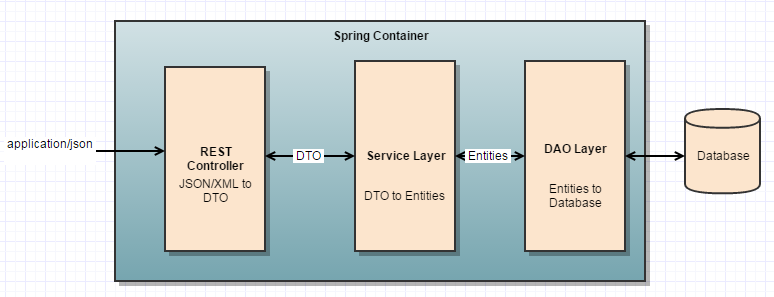
\includegraphics[width=\textwidth]{./images/Spring-REST-Web-Services.png} 

Bovenstaande afbeelding toont alle lagen die we ontwikkelen in een RESTful web applicatie. De RestController in de API-laag biedt REST-endpoints aan. De API-laag communiceert via DTO's of Data Transfer Objects met de servicelaag. De servicelaag implementeert alle bedrijfslogica. DTO's worden omgevormd naar entiteiten.  Entiteiten zijn  objecten uit het domein die we persisteren in de databank.  Deze entiteiten worden  doorgegeven aan de persistentielaag. De persistentielaag is verantwoordelijk voor het opslaan van de entiteiten in de database.

De Spring-container staat centraal in het Spring Framework. De container is verantwoordelijk voor het maken en beheren van objecten voor klassen die zijn geannoteerd met @Service, @Repository, ... De container zal deze objecten (beans) beschikbaar stellen wanneer ze nodig zijn.


\section{Een voorbeeld toepassing}

Dit hoofdstuk begeleidt je bij het ontwikkelen van een Spring Boot-toepassing waarbij we gegevens gaan wegschrijven naar en ophalen uit een databank. Je implementeert een RESTful web applicatie om de gegevens  maken om de informatie van de `Superhero Company' te beheren.  We zullen REST-endpoints implementeren voor het creëren,  aanpassen en verwijderen van superhelden. Later voeg je functionaliteit toe om missies voor de superhelden te creëren,  te updaten en te verwijderen. 

We gebruiken Spring Initializr om deze Spring Boot-toepassing op te zetten.

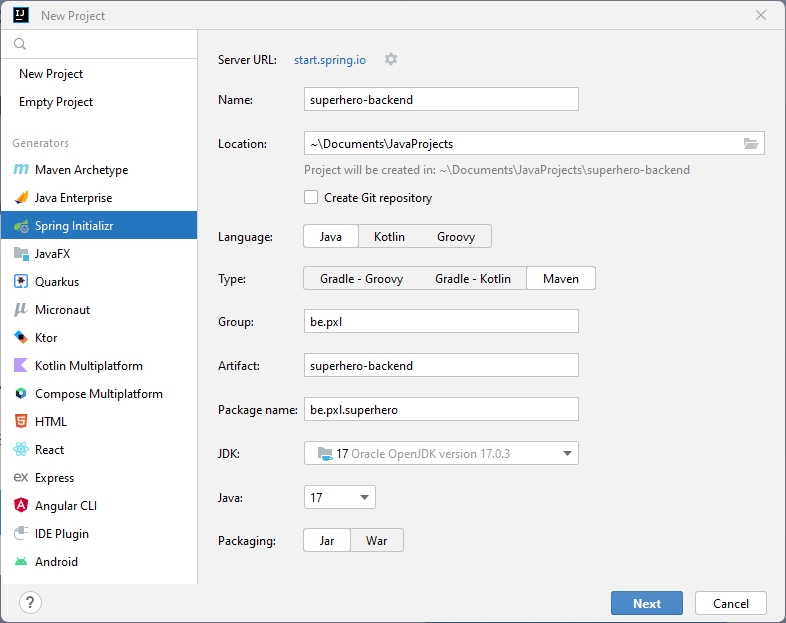
\includegraphics[width=\textwidth]{./images/chapter2/new_project.png} 

Vul de metadata voor het project in. Gebruik Maven als build tool. 


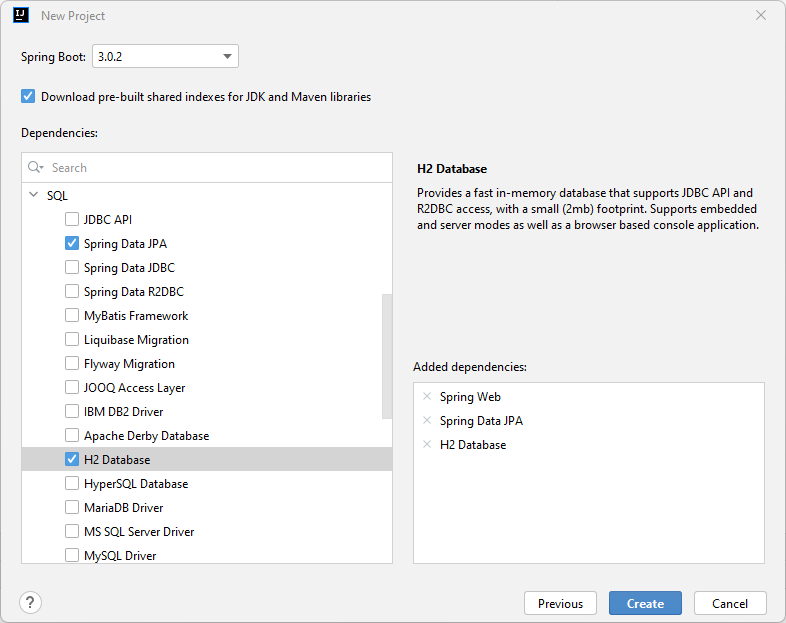
\includegraphics[width=\textwidth]{./images/chapter2/new_project_metadata.png}


\begin{oefening}
Maak het Spring Boot project met de naam `superhero-backend' aan.  Naast Spring Web en Spring Validation voeg je ook Spring Data JPA toe aan het project. Tenslotte voeg je nog de H2 Database dependency toe. Dit is een in-memory database en je hebt amper configuratie nodig om deze database te gebruiken. Dit is handig voor snelle prototyping, maar al je gegevens gaan verloren zodra je de toepassing opnieuw start.
\end{oefening}

\section{Gegevens opslaan en ophalen}

\subsection{Entiteitsklasse Superhero}

Allereerst hebben we een klasse nodig om de objecten te representeren die worden opgeslagen en opgehaald uit de database. Elk object van deze klasse zal overeenkomen met één rij van een tabel in de relationele database.
We implementeren de klasse Superheld. Om Superheld-objecten in de database op te slaan en deze later uit de database op te halen, annoteren we deze klasse als een entiteit. Een entiteitsklasse vertegenwoordigt een entiteit of object in het domeinmodel en wordt gemapt naar een tabel in de database. Elke instantie van deze klasse komt overeen met een rij in deze tabel, waardoor de eigenschappen van het object worden opgeslagen als kolommen in de database.

Hier is de enteitsklasse Superhero:

\begin{lstlisting}[frame=single]
package be.pxl.superhero.domain;

import jakarta.persistence.Entity;
import jakarta.persistence.GeneratedValue;
import jakarta.persistence.GenerationType;
import jakarta.persistence.Id;
import jakarta.persistence.Table;

@Entity
@Table(name="superheroes")
public class Superhero {
	
	@Id
	@GeneratedValue(strategy = GenerationType.IDENTITY)
	private Long id;
	
	private String firstName;
	private String lastName;
	private String superheroName;

	public Superhero() {
		// JPA only
	}

	public Superhero(String firstName, String lastName, String superheroName) {
		this.firstName = firstName;
		this.lastName = lastName;
		this.superheroName = superheroName;
	}

	public Long getId() {
		return id;
	}

	public String getFirstName() {
		return firstName;
	}

	public void setFirstName(String firstName) {
		this.firstName = firstName;
	}

	public String getLastName() {
		return lastName;
	}

	public void setLastName(String lastName) {
		this.lastName = lastName;
	}

	public String getSuperheroName() {
		return superheroName;
	}

	public void setSuperheroName(String superheroName) {
		this.superheroName = superheroName;
	}

	@Override
	public String toString() {
		return superheroName;
	}
}
\end{lstlisting}

De annotatie @Entity geeft aan dat de klasse Superhero een entiteitsklasse is. Spring is in staat om automatisch de databasetabel ('superheroes') te genereren met de nodige kolommen (velden) in de H2-database.
De primaire sleutel van de tabel is gemarkeerd met de annotatie @Id.  Met de annotatie @GeneratedValue(strategy = GenerationType.IDENTITY), hoeven we de primaire sleutels niet toe te wijzen aan de objecten. De database zelf is verantwoordelijk voor het genereren en toewijzen van de primaire sleutels.

\begin{oefening}
Voeg de enteitsklasse Superhero toe aan het project. Je voegt deze klasse toe in het package \textit{be.pxl.superhero.domain}.
\end{oefening}

\subsection{Repository}

Om query's in de database uit te voeren, hebben we een extra interface nodig die een \textbf{repository} wordt genoemd. Spring is in staat om automatisch databasequery's te genereren. Wanneer je de interface JpaRepository uitbreidt, zijn eenvoudige query's (zoals save, findById,...) al beschikbaar zonder dat je een regel code hoeft te schrijven.
De generieke interface JpaRepository hoeft alleen maar te weten welke gegevens het moet opslaan en ophalen.
Daarom moet het de naam van de entiteitsklasse en het gegevenstype van de primaire sleutel van de entiteitsklasse weten.

\begin{lstlisting}[frame=single]
package be.pxl.superhero.repository;

import be.pxl.superhero.domain.Superhero;
import org.springframework.data.jpa.repository.JpaRepository;
import org.springframework.stereotype.Repository;

@Repository
public interface SuperheroRepository extends JpaRepository<Superhero, Long> {
}
\end{lstlisting}



\begin{oefening}
Bestudeer de documentatie van de generieke interface JPARepository.
Voeg de repository SuperheroRepository toe  in het project.  Maak hiervoor het package \textit{be.pxl.superhero.repository} aan.
\end{oefening}

\subsection{Service-layer}

Zoals je al weet is de service-laag verantwoordelijk voor de implementatie van de businesslogica. De klassen in de service-laag zullen gebruik maken van repostories en andere service-klassen.  

Het is een goede idee om voor elke klasse in de servicelaag een interface te voorzien.
De serviceklassen mogen nooit entiteitsobjecten retourneren. We hebben DTO's (Data Transfer Objects) nodig om gegevens van de servicelaag naar de API-laag te sturen.

\begin{lstlisting}[frame=single]
package be.pxl.superhero.service;

import be.pxl.superhero.api.SuperheroDTO;
import be.pxl.superhero.api.SuperheroRequest;

import java.util.List;

public interface SuperheroService {

	List<SuperheroDTO> findAllSuperheroes();

	SuperheroDTO findSuperheroById(Long superheroId);

	Long createSuperhero(SuperheroRequest superheroRequest);

	SuperheroDTO updateSuperhero(Long superheroId, SuperheroRequest superheroRequest);

	boolean deleteSuperhero(Long superheroId);
}
\end{lstlisting}


\begin{lstlisting}[frame=single]
package be.pxl.superhero.api;

import be.pxl.superhero.domain.Superhero;

public class SuperheroDTO {

	private final Long id;
	private final String firstName;
    private final String lastName;
    private final String superheroName;

    public SuperheroDTO(Superhero superhero) {
	   this.id = superhero.getId();
        this.firstName = superhero.getFirstName();
        this.lastName = superhero.getLastName();
        this.superheroName = superhero.getSuperheroName();
    }

	public Long getId() {
		return id;
	}

	public String getFirstName() {
        return firstName;
    }

    public String getLastName() {
        return lastName;
    }

    public String getSuperheroName() {
        return superheroName;
    }

}
\end{lstlisting}

\begin{lstlisting}[frame=single]
package be.pxl.superhero.api;

public class SuperheroRequest {

	private String firstName;
	private String lastName;
	private String superheroName;

	public SuperheroRequest(String firstName, String lastName, String superheroName) {
		this.firstName = firstName;
		this.lastName = lastName;
		this.superheroName = superheroName;
	}

	public String getFirstName() {
		return firstName;
	}

	public void setFirstName(String firstName) {
		this.firstName = firstName;
	}

	public String getLastName() {
		return lastName;
	}

	public void setLastName(String lastName) {
		this.lastName = lastName;
	}

	public String getSuperheroName() {
		return superheroName;
	}

	public void setSuperheroName(String superheroName) {
		this.superheroName = superheroName;
	}

}

\end{lstlisting}

De klasse SuperheroServiceImpl, geannoteerd met @Service, biedt de implementatie voor de interface SuperheroService.
Alle CRUD-operaties (create-read-update-delete) voor Superhero-objecten worden hier aangeboden.
In de klasse SuperheroServiceImpl wordt alle bedrijfslogica geïmplementeerd. Als we bijvoorbeeld moeten controleren of de superheldennaam van een superheld uniek is, is deze klasse de plek om deze controle uit te voeren. 

De SuperheroRepository wordt door Spring Boot ter beschikking gesteld in de SuperheroServiceImpl. Daarom kan de serviceklasse gegevens opslaan en ophalen uit de database met behulp van deze repository.

\begin{lstlisting}[frame=single]
package be.pxl.superhero.service.impl;

import be.pxl.superhero.api.SuperheroDTO;
import be.pxl.superhero.api.SuperheroRequest;
import be.pxl.superhero.domain.Superhero;
import be.pxl.superhero.exception.ResourceNotFoundException;
import be.pxl.superhero.repository.SuperheroRepository;
import be.pxl.superhero.service.SuperheroService;
import org.springframework.stereotype.Service;

import java.util.List;
import java.util.stream.Collectors;

@Service
public class SuperheroServiceImpl implements SuperheroService {

	private final SuperheroRepository superheroRepository;

	@Autowired
	public SuperheroServiceImpl(SuperheroRepository superheroRepository) {
		this.superheroRepository = superheroRepository;
	}

	public List<SuperheroDTO> findAllSuperheroes() {
		return superheroRepository.findAll()
				.stream().map(SuperheroDTO::new)
				.toList();
	}

	public SuperheroDTO findSuperheroById(Long superheroId) {
		return superheroRepository.findById(superheroId)
		         .map(SuperheroDTO::new)
				.orElseThrow(() -> new ResourceNotFoundException("Superhero", "ID", superheroId));
	}

	public Long createSuperhero(SuperheroRequest superheroRequest) {
		Superhero superhero = new Superhero();
		superhero.setFirstName(superheroRequest.getFirstName());
		superhero.setLastName(superheroRequest.getLastName());
		superhero.setSuperheroName(superheroRequest.getSuperheroName());
		Superhero newSuperhero = superheroRepository.save(superhero);
		return newSuperhero.getId();
	}

	public SuperheroDTO updateSuperhero(Long superheroId, SuperheroRequest superheroRequest) {
		return superheroRepository.findById(superheroId).map(superhero -> {
			superhero.setFirstName(superheroRequest.getFirstName());
			superhero.setLastName(superheroRequest.getLastName());
			superhero.setSuperheroName(superheroRequest.getSuperheroName());
			return new SuperheroDTO(superheroRepository.save(superhero));
		}).orElseThrow(() -> new ResourceNotFoundException("Superhero", "id", superheroId));
	}

	public boolean deleteSuperhero(Long superheroId) {
		return superheroRepository.findById(superheroId)
				.map(superhero -> {
					superheroRepository.delete(superhero);
					return true;
				}).orElseThrow(() -> new ResourceNotFoundException("Superhero", "id", superheroId));

	}
}
\end{lstlisting}

\begin{lstlisting}
package be.pxl.superhero.exception;

@ResponseStatus(HttpStatus.NOT_FOUND)
public class ResourceNotFoundException extends RuntimeException {
    public ResourceNotFoundException(String resource, String field, String value) {
        super("Not found: " + resource + " with " + field + "=" + value);
    }

    public ResourceNotFoundException(String resource, String field, long value) {
        this(resource, field, Long.toString(value));
    }
}
\end{lstlisting}

\begin{oefening}
Maak het pakket \textit{be.pxl.superhero.api} aan en voeg het request-object SuperheroRequest en de DTO SuperheroDTO toe. Deze klassen worden gebruikt voor communicatie met de API-laag. Voeg de interface SuperheroService en de implementatie SuperheroServiceImpl toe aan je project. De interface bevindt zich in het pakket \textit{be.pxl.superhero.service}. De implementatie staat in het package \textit{be.pxl.superhero.service.impl}. Voeg tot slot de uitzonderingsklasse ResourceNotFoundException toe aan het package \textit{be.pxl.superhero.exception}.
\end{oefening}

\subsection{RESTController}

Nu kunnen we de REST-endpoints toevoegen voor het creëren, bijwerken, verwijderen en ophalen van superhelden.

Voor het creëren van een nieuwe superheld gebruiken we een POST-verzoek met een requestbody in JSON-formaat. Deze requestbody bevat alle informatie over de nieuwe superheld. Je hebt de klasse SuperheroRequest al aan het project toegevoegd. Deze klasse wordt gebruikt om de gegevens van de requestbody naar een object te mappen.

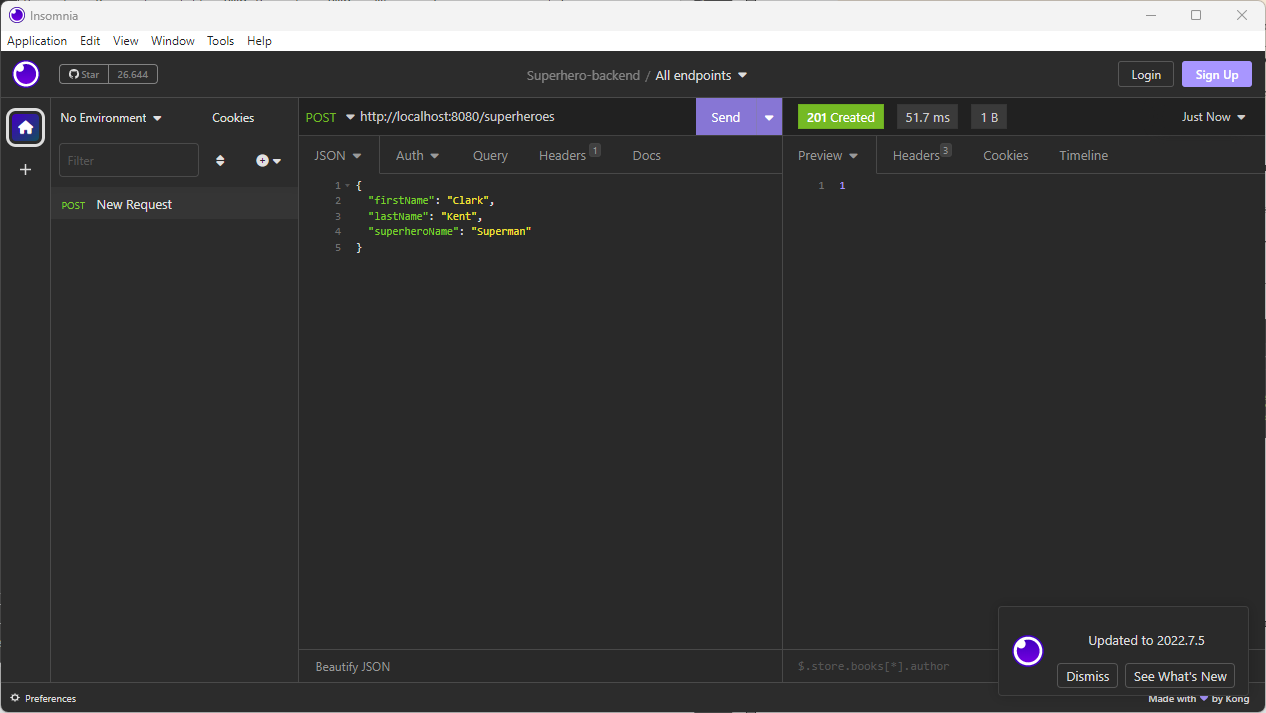
\includegraphics[width=\textwidth]{./images/chapter2/post-request-insomnia.png} 


\begin{lstlisting}[frame=single]
package be.pxl.superhero.api;

import be.pxl.superhero.service.SuperheroService;
import org.springframework.http.HttpStatus;
import org.springframework.http.ResponseEntity;
import org.springframework.web.bind.annotation.DeleteMapping;
import org.springframework.web.bind.annotation.GetMapping;
import org.springframework.web.bind.annotation.PathVariable;
import org.springframework.web.bind.annotation.PostMapping;
import org.springframework.web.bind.annotation.PutMapping;
import org.springframework.web.bind.annotation.RequestBody;
import org.springframework.web.bind.annotation.RequestMapping;
import org.springframework.web.bind.annotation.RestController;

import java.util.List;

@RestController
@RequestMapping("/superheroes")
public class SuperheroController {

	private final SuperheroService superheroService;

	public SuperheroController(SuperheroService superheroService) {
		this.superheroService = superheroService;
	}

	@GetMapping
	public List<SuperheroDTO> getSuperheroes() {
		return superheroService.findAllSuperheroes();
	}

	@GetMapping("/{superheroId}")
	public SuperheroDTO getSuperheroById(@PathVariable Long superheroId) {
		return superheroService.findSuperheroById(superheroId);
	}
	
	@PostMapping
	public ResponseEntity<Long> createSuperhero(@RequestBody SuperheroRequest superheroRequest) {
		return new ResponseEntity<>(superheroService.createSuperhero(superheroRequest), HttpStatus.CREATED);
	}
	
	@PutMapping("/{superheroId}")
	public SuperheroDTO updateSuperhero(@PathVariable Long superheroId, @RequestBody SuperheroRequest superheroRequest) {
		return superheroService.updateSuperhero(superheroId, superheroRequest);
	}
	
	@DeleteMapping("/{superheroId}")
	public ResponseEntity<Void> deleteSuperhero(@PathVariable Long superheroId) {
		boolean deleted = superheroService.deleteSuperhero(superheroId);
		return deleted? new ResponseEntity<>(HttpStatus.OK) : new ResponseEntity<>(HttpStatus.BAD_REQUEST);
	}
}
\end{lstlisting}

\begin{oefening}
Voeg @RestController SuperheroController toe aan je Spring Boot-toepassing. Herstart het project en maak een nieuwe superheld aan met Insomnia of Postman. Vervolgens roep je het REST-eindpunt aan om alle superhelden op te halen of om de superheld op te halen op basis van ID.

Hier is het JSON-formaat om een superheld te creëren:
\begin{lstlisting}
{
	"firstName": "Clark",
	"lastName": "Kent",
	"superheroName": "Superman"
}
\end{lstlisting}
\end{oefening}

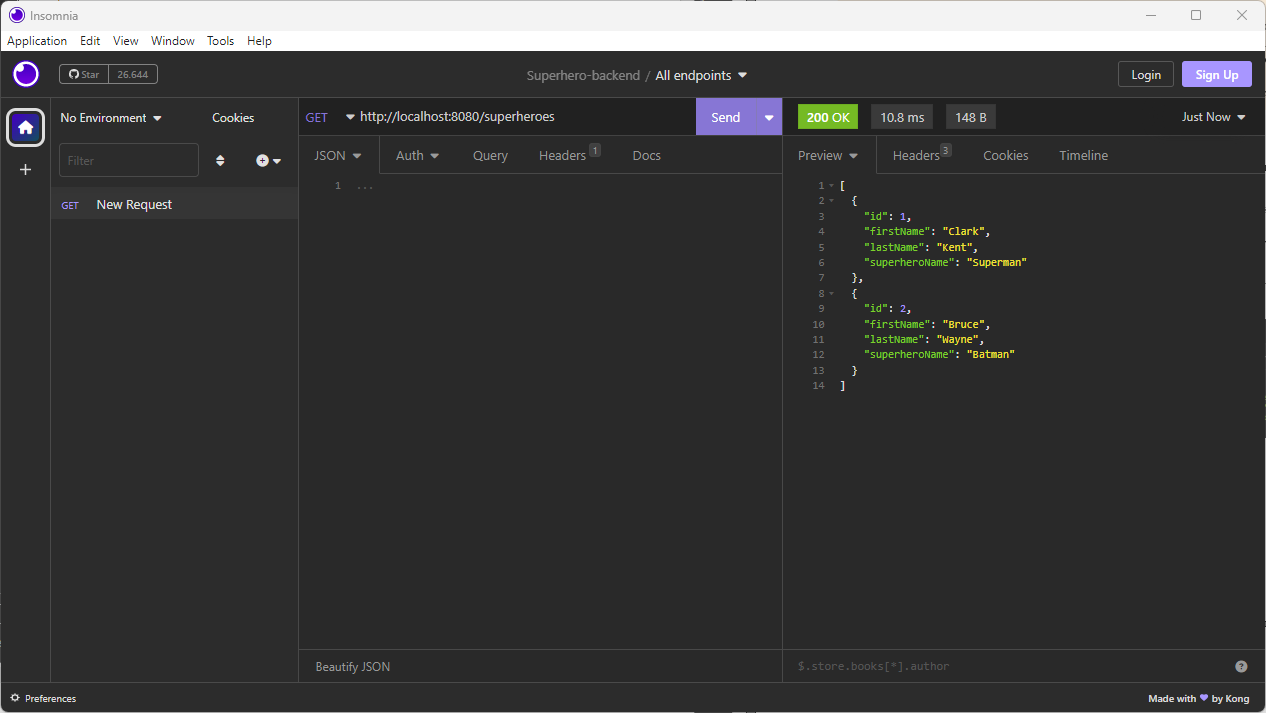
\includegraphics[width=\textwidth]{./images/chapter2/get-request-insomnia.png}

\section{URL context path}

Wanneer je een voorvoegsel (prefix), bijv. /api, aan alle URL's van de applicatie wilt toevoegen, kun je het volgende sleutel-waarde-paar toevoegen in het bestand application.properties:

\begin{lstlisting}[frame=single]
server.servlet.context-path=/api
\end{lstlisting}


\begin{oefening}
Verander het context-pad van je Spring Boot-applicatie. Het voorvoegsel /api moet worden gebruikt voor de applicatie. Herstart de applicatie en test de endpoints.
\end{oefening}

\section{API documentation}



\begin{lstlisting}[language=xml]
<dependency>
			<groupId>org.springdoc</groupId>
			<artifactId>springdoc-openapi-starter-webmvc-ui</artifactId>
			<version>2.2.0</version>
		</dependency>
\end{lstlisting}

De Swagger-documentatie in XML-formaat die te vinden is op de URL \url{http://localhost:8080/api/v3/api-docs} is niet gebruiksvriendelijk. Als je echter de URL \url{http://localhost:8080/api/swagger-ui.html} opent in je browser, kun je een gebruiksvriendelijke Swagger-pagina zien waar je zelfs je API kunt testen.

\begin{oefening}
Voeg swagger documentatie toe aan het project. Zoek eens op hoe je bijkomende Swagger documentatie in je RESTController kan toevoegen.
\end{oefening}


\begin{tcolorbox}[colback=blue!5!white,colframe=blue!75!black,title=H2 database]
De H2 in-memory database verdwijnt wanneer je de applicatie afsluit en alle data gaat verloren.
Je kunt bestanden gebruiken om de data permanent op te slaan. Als je de data van je in-memory database wilt bekijken, kun je de volgende eigenschap toevoegen aan het bestand application.properties:
\begin{lstlisting}[frame=single]
spring.h2.console.enabled=true
\end{lstlisting}
Als je de Spring Boot applicatie opstart, krijg je de unieke naam van de database. 
\begin{lstlisting}[frame=single]
H2 console available at '/h2-console'. Database available at 'jdbc:h2:mem:f5f92e54-3aff-4986-9d00-a0028b0eb6ed'
\end{lstlisting}
Als je de URL \url{http://localhost:8080/api/h2-console} in een browser browser open en de unieke naam van de databank invult en username ``sa'' en blanco paswoord ingeeft, dan krijg je toegang tot de tabellen en gegevens van de in-memory databank. 

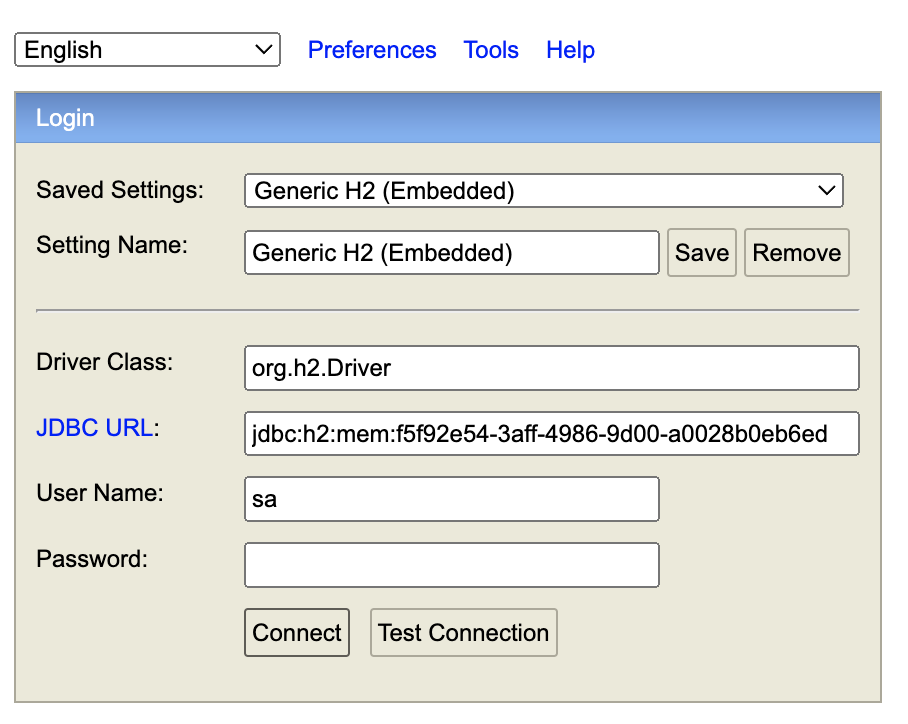
\includegraphics[width=\textwidth]{./images/chapter2/h2-database.png} 

\end{tcolorbox}

\section{Frontend}

Een frontend voor the superhero applicatie, geschreven in Angular,  kan je vinden op github.  (Credits to: \url{https://github.com/shoul10}).


 \fcolorbox{black}[HTML]{ADD8E6}{\parbox{\textwidth}{%
\noindent \textbf{Source code}\\
De frontend code is beschikbaar op: \url{https://github.com/custersnele/superhero-frontend.git}
}}

Zorg ervoor dat de nodige configuratie voorziet zodat de frontend de backend kan bereiken.  Denk eraan dat je ook CORS (Cross-Origin Resource Sharing) moet toestaan in je Spring Boot applicatie.

\begin{oefening}
Voeg CORS-ondersteuning toe aan je project. Voeg de configuratie toe in het package \textit{be.pxl.superhero.config}.  Herstart de Spring Boot applicatie.
Download de frontend code van github en open de code in een ontwikkelomgeving zoals   WebStorm.  Start de frontend toepassing op (ng serve) en cre\"er, update en verwijder je superhelden.
\end{oefening}

\chapter{Spring Data JPA}

\fcolorbox{black}[HTML]{E9F0E9}{\parbox{\textwidth}{%
\noindent \textbf{Learning goals}\\
The junior-colleague
\begin{enumerate}[nolistsep]
\item can describe the concept of ORM.
\item can explain what JPA is, and what it’s not.
\item can denominate different JPA providers.
\item can describe what a persistence unit is.
\item can explain the fundamental interfaces of JPA.
\item can explain what the persistence context is.
\item can implement entity classes.
\item can describe the entity objects’ lifecycle.
\item can implement different types of relationships between entity classes.
\item can implement CRUD operations.
\item can implement queries.
\item can implement named queries.
\item can explain, identify and solve the N + 1 query problem.
\end{enumerate}}}

  
\section{What is ORM?}

Object-Relational Mapping (ORM) is a technique that lets you query and manipulate data from a relational database using an object-oriented programming language.

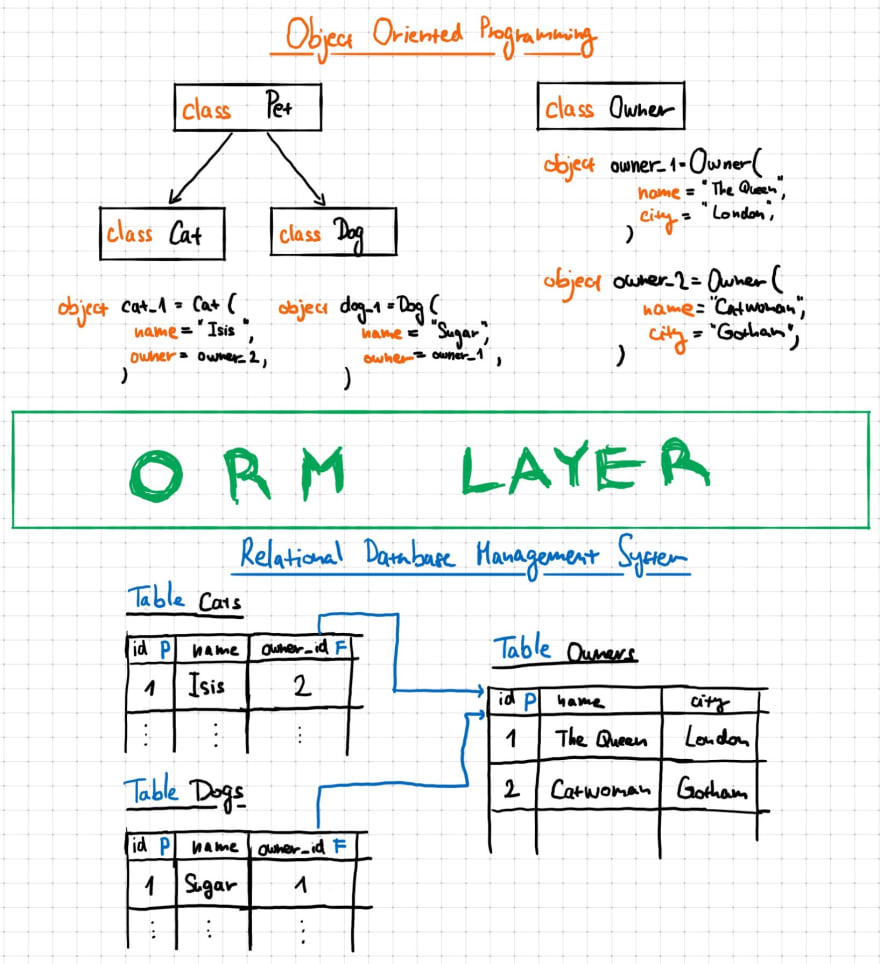
\includegraphics[width=\textwidth]{./images/chapter6/orm}


\section{What is JPA?}

The Java Persistence API (JPA; recently renamed to Jakarta Persistence API) is a specification that defines how to persist data in Java applications. JPA mainly focuses on the ORM layer and managing persistent objects.

JPA is a specification which means JPA consists of implementation guidelines for the Java ORM layer and the syntax. The specification only comes with interfaces, no actual implementation.  A reference implementation can be provided but other companies can create and distribute their own implementation of the specification.

\frame{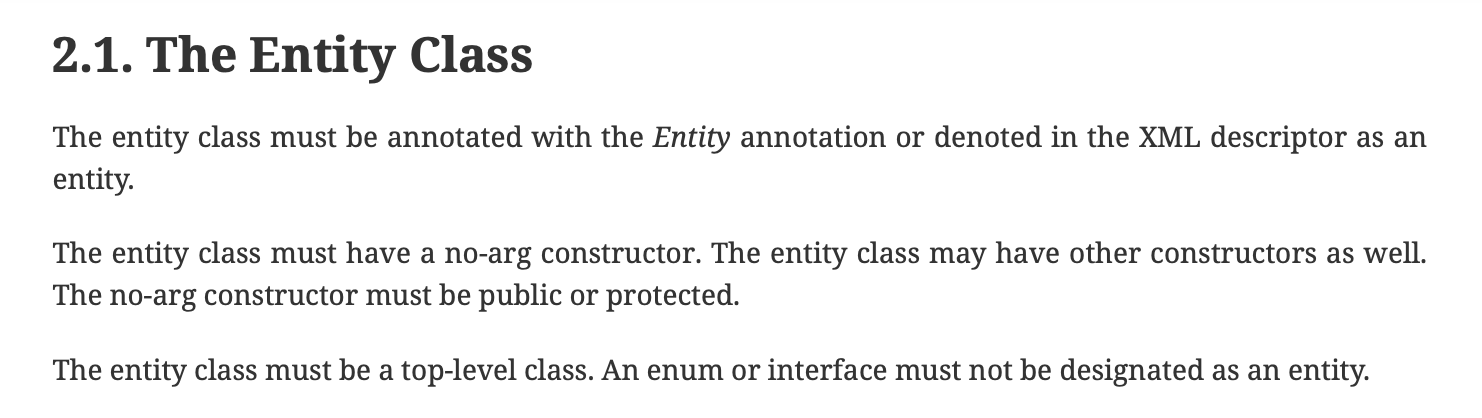
\includegraphics[width=\textwidth]{./images/chapter6/entity_class_specification}}

For our exercises and projects we will use Hibernate as the actual implementation of de JPA specification \footnote{\url{https://hibernate.org/ and https://hibernate.org/orm/}}.  

Spring Data JPA adds a layer on top of JPA. It uses all the features defined by the JPA specification, but adds no-code implementation of the repository pattern and the creation of database queries from method names.

JpaRepository extends PagingAndSortingRepository which in turn extends CrudRepository.

Their main functions are:

\begin{itemize}
\item CrudRepository mainly provides CRUD functions.
\item PagingAndSortingRepository provides methods to do pagination and sorting records.
\item JpaRepository provides some JPA-related methods such as flushing the persistence context and deleting records in a batch.
\end{itemize}


\section{Datasource}

In Spring Boot a DataSource-object is the preferred means of getting a connection to a database.
The interface jakarta.sql.DataSource is implemented by the database driver vendor. 

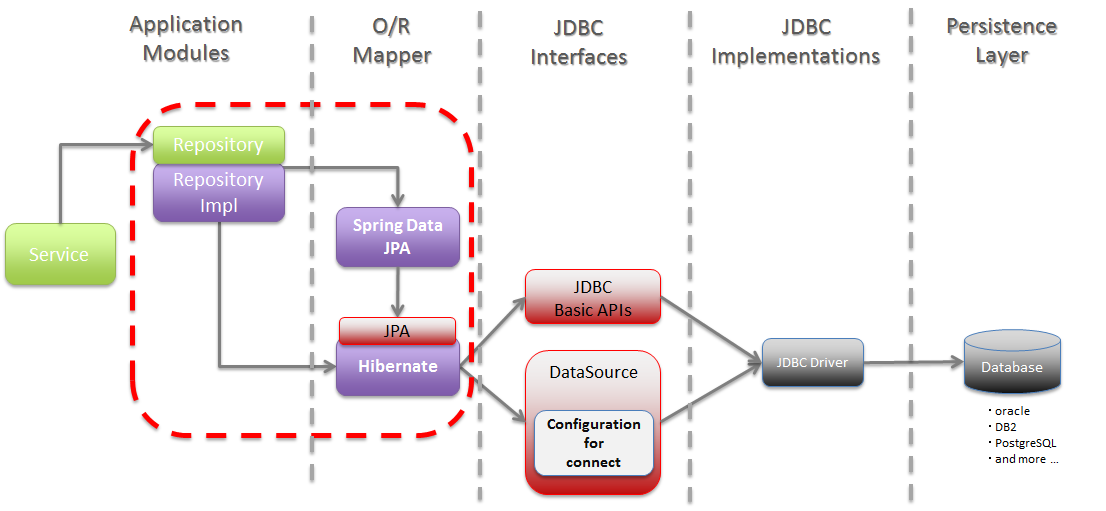
\includegraphics[width=\textwidth]{./images/chapter-jpa/springdatajpa}

The datasource can be specified in the application.properties file.
Here are some common database properties:

\begin{tabular}{|l|p{8cm}|}
\hline
spring.datasource.url & JDBC URL of the database.\\
spring.datasource.username & Login username of the database.\\
spring.datasource.password & Login password of the database.\\
spring.jpa.show-sql & Whether to enable logging of SQL statements. Default: false\\
spring.jpa.hibernate.ddl-auto & Possible values: none (production), create, create-drop, validate and update. \footnote{\url{https://stackoverflow.com/questions/42135114/how-does-spring-jpa-hibernate-ddl-auto-property-exactly-work-in-spring}}\\
\hline
\end{tabular}

Alternatively, the data source configuration can be programmatically.

The appropriate JDBC driver for your database must be included in your project. This is achieved by declaring the driver as a dependency in your project's Maven configuration file, pom.xml. The dependency ensures that the JDBC driver is available during runtime, allowing Spring Data JPA to establish and manage database connections.

Here is an example of how to include a JDBC driver for MySQL in your pom.xml file:

\begin{lstlisting}
<dependency>
<groupId>com.mysql</groupId>
<artifactId>mysql-connector-j</artifactId>
<scope>runtime</scope>
</dependency>
\end{lstlisting}

This configuration snippet includes the MySQL JDBC driver, mysql-connector-j.

Similarly,  to connect to a PostgreSQL database, you would use the PostgreSQL JDBC driver as shown below:

\begin{lstlisting}
<dependency>
<groupId>org.postgresql</groupId>
<artifactId>postgresql</artifactId>
<scope>runtime</scope>
</dependency>
\end{lstlisting}

Adjusting the driver version in your pom.xml may be necessary as you upgrade your database server or migrate to a newer version of Spring Data JPA.

\section{The Entity class}

\begin{lstlisting}[frame=single,language=java]
import jakarta.persistence.Entity;
import jakarta.persistence.Table;
import jakarta.persistence.Column;
import jakarta.persistence.Id;
import jakarta.persistence.GeneratedValue;
import jakarta.persistence.GenerationType;
import jakarta.persistence.Embedded;
import jakarta.persistence.Embeddable;

@Entity
@Table(name = "events")
public class Event {

    @Id
    @GeneratedValue(strategy = GenerationType.IDENTITY)
    private Long id;

    @Column(name = "name", nullable = false,  length = 200)
    private String title;

    @Embedded
    private EventDetails details;

    // Constructors, getters, and setters
}

@Embeddable
class EventDetails {
    private LocalDate date;
    @Column(length = 512)
    private String location;

    // Constructors, getters, and setters
}
\end{lstlisting}

A JPA entity class is a POJO (Plain Old Java Object) class  that is annotated as having the ability to represent objects in the database.
The \textbf{@Entity} annotation is used to declare that a class is an entity, so JPA will manage it and map it to a database table.

\textbf{@Table} specifies the table in the database with which the entity is mapped.

The \textbf{@Id} annotation marks a field as a primary key field.

The \textbf{@GeneratedValue} annotation is used to configure the primary key generation strategy for an entity. This annotation is usually combined with @Id to specify that the persistence provider should automatically generate a unique identifier for the entity objects. There are several strategies defined in the GenerationType enumeration that can be used with @GeneratedValue. Here's an overview:

\begin{itemize}
\item \textbf{GenerationType.AUTO}

This is the default strategy and the persistence provider will choose the generation strategy based on the specific database capabilities and dialect. 

\item \textbf{GenerationType.IDENTITY}

Indicates that the persistence provider must assign primary keys using the database identity column. This is typically supported by SQL databases with an auto-increment column.

\item \textbf{GenerationType.SEQUENCE}

Specifies that the primary key values will be generated using a database sequence. This is a special database object that generates numbers in sequential order. Not all databases support sequences.
This strategy is useful for databases supporting sequences, like Oracle, PostgreSQL, etc. It's beneficial for high-volume applications due to better performance compared to IDENTITY, as the sequence generation can be more efficiently managed.

\item \textbf{GenerationType.TABLE}

Uses a database table to simulate a sequence. This strategy uses a table to hold the next id incrementally. It's a portable solution but not as efficient as using database-specific features like sequences or identity columns.
\end{itemize}

The \textbf{@Column} annotation is used to specify the details of the column to which a field or property will be mapped. You can use column annotation with the following most commonly used attributes:
\begin{itemize}
\item \textbf{name}: specify the name of the column.
\item \textbf{length}: specify the size of thee column, particularly for a String value.
\item \textbf{nullable}: mark the column to be NOT NULL when the database schema is generated.
\item \textbf{unique}: mark the column to contain only unique values.
\end{itemize}


The \textbf{@Embeddable} annotation marks a class to be embedded within another entity.
In this example,  the EventDetails does not need its own table; instead, its properties are incorporated into the table of the entity that embeds it.

The annotation \textbf{@Embedded}  is used to denote a class whose instances are stored as an intrinsic part of an owning entity.
 All the fields of EventDetails class are embedded within the events table, avoiding the need for a separate table.


\section{Entity lifecycle}

The EntityManager is a core interface of JPA.  An instance of EntityManager is used to create and remove  entity instances, to find entities by their primary key,  and to query over entities.  In fact,  an instance of the EntityManager is used to interact with the persistence context. 

The persistence context is one of the main concepts in JPA.
It is a set of all entity object that you are currently using or used recently. You can think of the persistence context as some kind of first-level cache. Each entity object in the persistence context represents a record in the database.
The persistence context manages these entity objects and their lifecycle. Each entity object has one of 4 states: new, managed, removed, and detached.

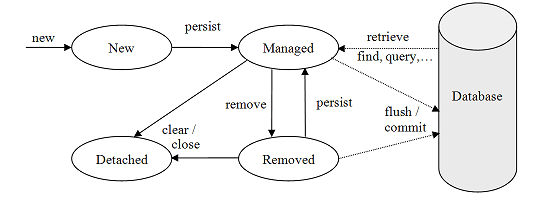
\includegraphics[width=\textwidth]{./images/chapter6/entity_states}

A newly instantiated entity object is in state \textbf{new} or \textbf{transient}. The entity object hasn't been persisted yet, so there's no database record yet. The persistence context does not know about the entity object yet. 

All entity objects that attached to the persistence context are in the lifecycle state \textbf{managed}. An entity object becomes managed when it is persisted to the database. Entity object retrieved from the database are also in the managed state.
If a managed entity object is modified (updated) within an active transaction, the change is detected by the persistence context and passed on to the database.

When a managed entity is removed within an active transaction, the state changes from managed to removed, and the record is physically deleted from the database (when the transaction commits).

An entity gets detached when it is no longer managed by the persistence context but still represents a record in the database.
Detached objects are limited in functionality.

 
Programmatically we need to use the entitymanager to change the state of the entity object in the persistence context which results in changes or updates in our database. 

When using Spring Data JPA you don't have to implement the interaction with the entitymanager. When you create a Repository, the SimpleJpaRepository class provided by Spring Data JPA provides the default implementation. SimpleJpaRepository class internally uses JPA entitymanager.

\begin{oefening}
Open the class SimpleJpaRepository and take a look at its implementation (e.g. save()-method).
\end{oefening}


\section{Relationships}

\subsection{OneToOne relationship}

A OneToOne relationship in JPA is used when one entity instance is associated with exactly one instance of another entity.  In this example a user has exactly one passport.

In a \textbf{uni-directional} OneToOne relationship, only one side of the relationship maintains knowledge of the other side’s existence. Consider a scenario where each Person has exactly one Passport. The Person entity holds a reference to the Passport, but the Passport does not hold any reference to the Person.

\begin{lstlisting}
@Entity
public class Person {
    @Id
    @GeneratedValue(strategy = GenerationType.IDENTITY)
    private Long id;
    
    @OneToOne(cascade = CascadeType.ALL)
    @JoinColumn(name = "passport_id", referencedColumnName = "id")
    private Passport passport;

    // Standard getters and setters
}

@Entity
public class Passport {
    @Id
    @GeneratedValue(strategy = GenerationType.IDENTITY)
    private Long id;
    
    private String number;

    // Standard getters and setters
}
\end{lstlisting}

In this example, the Person entity contains a Passport field annotated with @OneToOne. The @JoinColumn annotation specifies the column in the Person table that joins to the primary key of the Passport entity.

The concept of \"cascade types\" defines how persistence operations such as save, delete, and update performed on one entity should be propagated (or cascaded) to its associated entity. 

When using the @OneToOne annotation in JPA, you can specify a cascade type to automate the persistence lifecycle management of the associated entity. Here are the most common cascade types used in JPA:

\begin{itemize}
\item \textbf{CascadeType.PERSIST}: When persisting an entity, also persist the associated entity.  For example, when saving a Person object, also save its associated Passport.

\item \textbf{CascadeType.MERGE}: When merging the state of an entity into the current persistence context, also merge the entity held in this field.

\item \textbf{CascadeType.REMOVE}: When deleting an entity, also delete the associated entity. This is particularly useful when the associated entity no longer makes sense to exist independently.

\item \textbf{CascadeType.REFRESH}: When refreshing an entity, also refresh the entities held in this field. This means reloading the content of the associated entity from the database, which can be useful if the database might be changed by other processes.

\item \textbf{CascadeType.DETACH}: When an entity is detached from the persistence context, also detach the entities held in this field.

\item \textbf{CascadeType.ALL}: A convenience that cascades all the above operations (PERSIST, MERGE, REMOVE, REFRESH, DETACH). Using CascadeType.ALL is common for @OneToOne and @OneToMany associations.
\end{itemize}

In a \textbf{bi-directional} OneToOne relationship, both entities are aware of each other. This relationship allows navigation from either side. Using the same example as above, both the Person and Passport entities can have references to each other.

\begin{lstlisting}
@Entity
public class Person {
    @Id
    @GeneratedValue(strategy = GenerationType.IDENTITY)
    private Long id;

    @OneToOne(mappedBy = "person", cascade = CascadeType.ALL)
    private Passport passport;

    // Standard getters and setters
}

@Entity
public class Passport {
    @Id
    @GeneratedValue(strategy = GenerationType.IDENTITY)
    private Long id;

    private String number;

    @OneToOne
    @JoinColumn(name = "person_id")
    private Person person;

    // Standard getters and setters
}
\end{lstlisting}

In this bi-directional setup, the Person entity uses the mappedBy attribute in the @OneToOne annotation to indicate that the Person is not the owner of the relationship and that the Passport entity contains the foreign key.

\subsection{ManyToOne relationship}

A ManyToOne relationship in JPA is commonly used when one entity is related to multiple instances of another entity. For instance, in a blog system, many posts may belong to one category.

Uni-directional ManyToOne Relationship
In a uni-directional ManyToOne relationship, only the 'many' side of the relationship is aware of the 'one' side. This setup is often seen when the 'one' side doesn't need to directly access the 'many' side.

Example: Books and Authors
Suppose each book can have one author, but each author can write many books. Here, the relationship from books to authors is a typical example of a uni-directional ManyToOne relationship.

\begin{lstlisting}
@Entity
public class Book {
    @Id
    @GeneratedValue(strategy = GenerationType.IDENTITY)
    private Long id;

    private String title;

    @ManyToOne
    @JoinColumn(name = "author_id", nullable = false)
    private Author author;

    // Standard getters and setters
}

@Entity
public class Author {
    @Id
    @GeneratedValue(strategy = GenerationType.IDENTITY)
    private Long id;

    private String name;

    // Standard getters and setters, no reference back to Book
}
\end{lstlisting}

In this model, each Book entity holds a reference to its Author, which is annotated with @ManyToOne. The @JoinColumn annotation specifies the foreign key column in the Book table that links to the Author.

Repository Configuration
Repositories for each entity can be defined as follows:

\begin{lstlisting}
public interface BookRepository extends JpaRepository<Book, Long> {
}

public interface AuthorRepository extends JpaRepository<Author, Long> {
}
\end{lstlisting}

Bi-directional ManyToOne Relationship
In a bi-directional relationship, both sides of the relationship are aware of each other. This is useful when you want to navigate the relationship from either side.

Example: Books and Authors Continued
Expanding on the previous example, suppose now we want authors to also be aware of the books they've written.

Entity Definition
\begin{lstlisting}
@Entity
public class Book {
    @Id
    @GeneratedValue(strategy = GenerationType.IDENTITY)
    private Long id;

    private String title;

    @ManyToOne
    @JoinColumn(name = "author_id", nullable = false)
    private Author author;

    // Standard getters and setters
}

@Entity
public class Author {
    @Id
    @GeneratedValue(strategy = GenerationType.IDENTITY)
    private Long id;

    private String name;

    @OneToMany(mappedBy = "author")
    private Set<Book> books = new HashSet<>();

    // Standard getters and setters
}
\end{lstlisting}

In this bi-directional setup, the Author class includes a Set<Book> to hold the collection of books. The @OneToMany annotation in Author uses the mappedBy attribute to indicate that the Author entity is not the owner of the relationship and that the Book entity contains the foreign key.

\subsection{ManyToMany relationship}


A ManyToMany relationship is used when multiple instances of one entity are associated with multiple instances of another entity. Using the example of books and authors, a ManyToMany relationship would be appropriate if each book could have multiple authors and each author could write multiple books. 

In a uni-directional ManyToMany relationship, only one entity maintains the relationship information.

Imagine a scenario where each book can have multiple authors, but we are only interested in navigating from books to authors and not the other way around.

\begin{lstlisting}
@Entity
public class Book {
    @Id
    @GeneratedValue(strategy = GenerationType.IDENTITY)
    private Long id;

    private String title;

    @ManyToMany
    @JoinTable(
        name = "book_author",
        joinColumns = @JoinColumn(name = "book_id"),
        inverseJoinColumns = @JoinColumn(name = "author_id")
    )
    private Set<Author> authors = new HashSet<>();

    // Standard getters and setters
}

@Entity
public class Author {
    @Id
    @GeneratedValue(strategy = GenerationType.IDENTITY)
    private Long id;

    private String name;

    // Standard getters and setters, no reference back to Books
}
\end{lstlisting}
In this example, the Book entity defines a ManyToMany relationship to the Author entity. The @JoinTable annotation specifies the table that maps books to authors, including columns for each foreign key.


In a bi-directional ManyToMany relationship, both entities are aware of each other, and navigation is possible from either side.

This time, both books and authors are aware of each other and can navigate the relationship.

\begin{lstlisting}
@Entity
public class Book {
    @Id
    @GeneratedValue(strategy = GenerationType.IDENTITY)
    private Long id;

    private String title;

    @ManyToMany
    @JoinTable(
        name = "book_author",
        joinColumns = @JoinColumn(name = "book_id"),
        inverseJoinColumns = @JoinColumn(name = "author_id")
    )
    private Set<Author> authors = new HashSet<>();

    // Standard getters and setters
}

@Entity
public class Author {
    @Id
    @GeneratedValue(strategy = GenerationType.IDENTITY)
    private Long id;

    private String name;

    @ManyToMany(mappedBy = "authors")
    private Set<Book> books = new HashSet<>();

    // Standard getters and setters
}
\end{lstlisting}

In the bi-directional arrangement, the Author entity includes a Set<Book> to hold the collection of books. The mappedBy attribute indicates that the Author is not the owner of the relationship, and the mapping details are managed by the Book entity.

\section{Fetching strategy}

JPA provides two main fetching strategies to control how related entities are loaded from the database:

\begin{itemize}
\item \textbf{Eager Fetching}: With eager fetching, related entities are loaded immediately with the main entity, whether they are accessed in the application or not. This can lead to performance issues if the relationships involve large sets of data. Eager fetching is often used when the data sets are small or always used together with the main entity.

\item \textbf{Lazy Fetching}: Lazy fetching loads the related entities only when they are explicitly accessed in the application. This can improve performance by reducing the initial load time and the amount of memory consumed. However, it requires careful management of the persistence context to avoid LazyInitializationException.
\end{itemize}

java
Copy code
@ManyToMany(fetch = FetchType.LAZY)
private Set<Author> authors = new HashSet<>();
In the case of ManyToMany relationships, the default fetching strategy is lazy because eager fetching can result in very large numbers of joins and thus severe performance degradation.

Understanding and choosing the right fetching strategy based on the specific use case and data access patterns is crucial for developing efficient, scalable applications.

Consider the following method findBooksByAuthor() in a BookService.
When we look closely at the logging of the SQL-queries. We see that first, the author is retrieved and later, the author's books are retrieved on the moment we call author.getBooks(), not sooner. This is lazy loading or lazy fetching. When dealing with one-to-many or many-to-many relationships, lazy fetching is mostly the best solution in terms of performance.

\begin{lstlisting}
@Service
public class BookService {

    private static final Logger LOGGER = LogManager.getLogger(BookService.class);

    private final AuthorRepository authorRepository;

    public BookService(AuthorRepository authorRepository) {
        this.authorRepository = authorRepository;
    }

    public List<String> getBooksByAuthor(String authorName) {
        Author author = authorRepository.findAuthorByName(authorName).orElseThrow(() -> new NotFoundException("No author found"));
        LOGGER.info("Author retrieved...");
        return author.getBooks().stream().map(Book::getTitle).toList();
    }
}
\end{lstlisting}

\begin{verbatim}
2024-04-23T20:23:48.883+02:00  INFO 26656 --- [nio-8080-exec-8] be.pxl.helpdesk.service.BookService      : Starting getBooksByAuthor
Hibernate: 
    select
        a1_0.id,
        a1_0.name 
    from
        authors a1_0 
    where
        a1_0.name=?
2024-04-23T20:23:48.946+02:00  INFO 26656 --- [nio-8080-exec-8] be.pxl.helpdesk.service.BookService      : Author retrieved...
Hibernate: 
    select
        b1_0.author_id,
        b1_1.id,
        b1_1.title 
    from
        book_authors b1_0 
    join
        books b1_1 
            on b1_1.id=b1_0.book_id 
    where
        b1_0.author_id=?
\end{verbatim}

If we change the relationship between Author and Books to eager fetching, the books are retrieved on the moment we search the author by its name.


\begin{lstlisting}
@Entity
@Table(name = "authors")
public class Author {
    @Id
    @GeneratedValue(strategy = GenerationType.IDENTITY)
    private Long id;

    private String name;

    @ManyToMany(mappedBy = "authors", fetch = FetchType.EAGER)
    private Set<Book> books = new HashSet<>();

    // Standard getters and setters

    public void addBook(Book book) {
        books.add(book);
    }

    public Set<Book> getBooks() {
        return books;
    }
}
\end{lstlisting}

\begin{verbatim}
2024-04-23T20:21:02.145+02:00  INFO 19956 --- [nio-8080-exec-6] be.pxl.helpdesk.service.BookService      : Starting getBooksByAuthor
Hibernate: 
    select
        a1_0.id,
        a1_0.name 
    from
        authors a1_0 
    where
        a1_0.name=?
Hibernate: 
    select
        b1_0.author_id,
        b1_1.id,
        b1_1.title 
    from
        book_authors b1_0 
    join
        books b1_1 
            on b1_1.id=b1_0.book_id 
    where
        b1_0.author_id=?
2024-04-23T20:21:02.216+02:00  INFO 19956 --- [nio-8080-exec-6] be.pxl.helpdesk.service.BookService      : Author retrieved...
\end{verbatim}

Always be very carefull with bi-directional relationships and eager fetching. The performance cost may be underestimated. In this case, if an author has written many books, it may be beneficial, to only maintain the owning part of the relationship and search for in author's books with a query in the BookRepository.

\section{Transactions}

The @Transactional Annotation in Spring Boot
The @Transactional annotation in Spring Boot is used to declare that a method or a class should be executed within a transactional context. This is a powerful feature provided by the Spring Framework that manages the transaction management boilerplate that can complicate the application code and ensures that your transaction requirements are handled consistently.

Key Concepts:
Transaction: A sequence of actions that are treated as a single unit of work. These actions should either complete entirely or take no effect at all.
Transaction Management: Ensures that an application maintains data integrity and consistency in scenarios involving multiple transaction operations.
Usage of @Transactional
At the method level: When placed above a method, @Transactional ensures the method executes within a transaction. If a transaction is already running, the method by default runs within that transaction.
At the class level: If @Transactional is placed at the class level, it applies to all the public methods of that class.
Transaction Propagation
Transaction propagation behavior defines how transactions relate to each other. Common propagation types include:

REQUIRED: Use the current transaction or start a new one if none exists.
REQUIRES\_NEW: Always start a new transaction, suspending the current one if it exists.
SUPPORTS: Run within the current transaction if it exists; otherwise, run non-transactionally.
NEVER: Ensure no current transaction exists, throwing an exception if one exists.
Flowchart of How Transactions Work in Spring Boot
Here’s a simplified flowchart illustrating how transactions are managed in Spring Boot using the @Transactional annotation:

Method Invocation: A method annotated with @Transactional is called.
Check Existing Transaction: The transaction manager checks if a current transaction exists.
Transaction Propagation: Depending on the propagation setting:
Use current transaction or start a new one.
Suspend the current transaction and start a new one.
Run without a transaction if none exists.
Method Execution: The method executes. Database operations are performed as part of the transaction.
Commit/Rollback:
If the method completes successfully, the transaction is committed.
If an exception occurs, the transaction is rolled back.
Example: Book and Author Entities
Let’s consider an example with Book and Author entities. We want to ensure that adding a book linked to an author is transactional (either both the book and the author are saved, or neither).

Entity Classes
java
Copy code
@Entity
public class Author {
    @Id
    @GeneratedValue(strategy = GenerationType.AUTO)
    private Long id;
    private String name;
    // constructors, getters, and setters
}

@Entity
public class Book {
    @Id
    @GeneratedValue(strategy = GenerationType.AUTO)
    private Long id;
    private String title;
    @ManyToOne
    private Author author;
    // constructors, getters, and setters
}
Service Class with Transactional Methods
java
Copy code
@Service
public class LibraryService {
    @Autowired
    private BookRepository bookRepository;
    @Autowired
    private AuthorRepository authorRepository;

    @Transactional
    public void addBookAndAuthor(Book book, Author author) {
        authorRepository.save(author); // Save author
        book.setAuthor(author);
        bookRepository.save(book); // Save book
        // Both saves are part of the same transaction
    }
}

\section{Queries}

Basic CRUD queries are in Spring Data JPA available in the repositories. But there are multiple ways of creating custom queries in a Spring boot application. Let's discuss the different
types of queries.

\subsection{Query methods}

Spring Data JPA can create queries based on method names. You can use keywords like \textit{findBy}, \textit{findAllBy},
\textit{findBy...And...}, ...

An overview of the keywords can be found in spring documentation \url{https://docs.spring.io/spring-data/jpa/reference/jpa/query-methods.html}.

\begin{lstlisting}
public interface ProductRepository extends JpaRepository<Product, Long> {
    // Query method with parameters for finding products by name and price
    List<Product> findByNameAndPrice(String name, double price);
}
\end{lstlisting}

\subsection{JPQL queries}

JPQL, or Java Persistence Query Language, is a query language designed to abstract database details from the developer, allowing queries to be written based on entity model classes rather than on database tables.


\begin{lstlisting}
public interface UserRepository extends JpaRepository<User, Long> {
  @Query("SELECT u FROM User u WHERE u.age >= :minAge")
  List<User> findByAgeGreaterThan(@Param("minAge") int minAge);
}
\end{lstlisting}

\subsection{Native SQL queries}

\begin{lstlisting}

\end{lstlisting}


\section{Unit testing a repository}

Spring Data JPA offers an annotation @DataJpaTest which makes repository testing possible with a minimum of configuration. 

Add the h2 dependency with scope test in your pom.xml. This way the unit test for your repository will use the h2 database to test your queries.

\begin{lstlisting}
<dependency>
	<groupId>com.h2database</groupId>
	<artifactId>h2</artifactId>
	<scope>test</scope>
</dependency>
\end{lstlisting}

The builder pattern is used in this example to create entity objects for testing purpose. These entity objects are stored in the in-memory database. There is an IntelliJ IDEA plugin that generates the builder-classes for you (Generate Builder plugin).

\begin{lstlisting}
public final class AuthorBuilder {
    private String name;
    private Set<Book> books;

    private AuthorBuilder() {
    }

    public static AuthorBuilder anAuthor() {
        return new AuthorBuilder();
    }

    public AuthorBuilder withName(String name) {
        this.name = name;
        return this;
    }

    public AuthorBuilder withBooks(Set<Book> books) {
        this.books = books;
        return this;
    }

    public Author build() {
        Author author = new Author();
        author.setName(name);
        author.setBooks(books);
        return author;
    }
}
\end{lstlisting}

The @DataJpaTest annotation is used to test JPA repositories in Spring Boot applications. It’s a specialized test annotation that provides a minimal Spring context for testing the persistence layer. 

By default, each test method annotated with @DataJpaTest runs within a transactional boundary. This ensures that changes made to the database are automatically rolled back at the end of the test, leaving a clean slate for the next test.

The test class uses the entity managers, which is injected in the test with the @PersistenceContext annotation. The flush() forces to synchronize the persistence context to the database. The clear() empties the persistence context. Therefore, all entities are detached and can be fetched from the database.


\begin{lstlisting}[frame=single, language=java]
package be.pxl.helpdesk.repository;

import be.pxl.helpdesk.builder.AuthorBuilder;
import be.pxl.helpdesk.domain.Author;
import jakarta.persistence.EntityManager;
import jakarta.persistence.PersistenceContext;
import org.junit.jupiter.api.BeforeEach;
import org.junit.jupiter.api.Test;
import org.springframework.beans.factory.annotation.Autowired;
import org.springframework.boot.test.autoconfigure.orm.jpa.DataJpaTest;

import java.util.Arrays;
import java.util.Optional;

import static org.junit.jupiter.api.Assertions.assertEquals;
import static org.junit.jupiter.api.Assertions.assertTrue;

@DataJpaTest
public class AuthorRepositoryTest {

	@PersistenceContext
	protected EntityManager entityManager;

	@Autowired
	private AuthorRepository authorRepository;

	private final Author author1 = AuthorBuilder.anAuthor().withName("Famous Author").build();


	private final Author author2 = AuthorBuilder.anAuthor().withName("Not So Famous Author").build();

	@BeforeEach
	public void init() {
		authorRepository.saveAll(Arrays.asList(author1, author2));
		entityManager.flush();
		entityManager.clear();
	}

	@Test
	public void returnsAuthorByName() {
		Optional<Author> author = authorRepository.findAuthorByName("Famous Author");

		assertTrue(author.isPresent());
		assertEquals("Famous Author", author.get().getName());
	}

	@Test
	public void returnsEmptyOptionalWhenNoAuthorPlayerWithName() {
		Optional<Author> author = authorRepository.findAuthorByName("Bestseller Author");

		assertTrue(author.isEmpty());
	}
}
\end{lstlisting}


\section{Pagination}

Pageable is an interface provided by Spring Data that contains information about the pagination and sorting of data. It helps in structuring the way data is retrieved from the database in manageable chunks or pages, rather than pulling large quantities of data all at once, which can be inefficient and slow.


\begin{lstlisting}
@RestController
@RequestMapping("books")
public class BookController {

    private final BookService bookService;

    public BookController(BookService bookService) {
        this.bookService = bookService;
    }

    @GetMapping("search")
    public List<BookDto> searchBooks(@RequestBody FilterDto filter) {
        return bookService.searchBooks(filter);
    }

    @GetMapping
    public Page<BookDto> getBooks(Pageable pageable) {
        return bookService.findAllBooks(pageable);
    }
}
\end{lstlisting}

The parameter Pageable is automatically populated by Spring when the method is called. The Pageable object typically includes:
\begin{itemize}
\item page: The current page number (0-indexed, where 0 is the first page).
\item size: The number of records per page.
\item sort: Criteria for sorting the data (optional).
\end{itemize}

For example, a request URL might look like this: \textit{/books?page=0\&size=10\&sort=title,asc}. This tells the application to get the first page of books, with 10 books per page, sorted by title in ascending order.

\begin{lstlisting}
@Service
public class BookService {

    private static final Logger LOGGER = LogManager.getLogger(BookService.class);

    private final AuthorRepository authorRepository;
    private final BookRepository bookRepository;

    public BookService(AuthorRepository authorRepository, BookRepository bookRepository) {
        this.authorRepository = authorRepository;
        this.bookRepository = bookRepository;
    }

    public List<String> getBooksByAuthor(String authorName) {
        LOGGER.info("Starting getBooksByAuthor");
        Author author = authorRepository.findAuthorByName(authorName).orElseThrow(() -> new NotFoundException(""));
        LOGGER.info("Author retrieved...");
        return author.getBooks().stream().map(Book::getTitle).toList();
    }

    public Page<BookDto> findAllBooks(Pageable pageable) {
        Page<Book> books = bookRepository.findAll(pageable);
        return books.map(this::mapToBookDto);
    }


    private BookDto mapToBookDto(Book book) {
        return new BookDto(book.getTitle(), book.getCategory(), book.getAuthors().stream().map(Author::getName).toList());
    }
}
\end{lstlisting}

The Pageable parameter is passed to the bookService.findAllBooks(pageable) method. This method is expected to interact with the repository layer that extends Spring Data’s PagingAndSortingRepository or JpaRepository. These repositories natively support Pageable for pagination and sorting.
The repository method would use the Pageable object to construct a database query that fetches only the specified slice of data based on the page number, page size, and sorting criteria.
Return Type (Page<BookDto>):
The method returns a Page<BookDto>, which is a specialized implementation of the Slice interface. It provides not only the list of data for the current page but also additional information about the total number of pages, the total number of elements, whether there are more pages available, and so forth.
Benefits of Using Pageable
Efficiency: Only the necessary slice of data is fetched from the database, which can be crucial for performance when dealing with large datasets.
Flexibility: Clients of your API can specify how many records they want per page and how the data should be sorted.
Ease of Use: Spring Data handles much of the heavy lifting, making it easier to implement robust pagination and sorting without much boilerplate code.


\begin{lstlisting}

\end{lstlisting}

\begin{verbatim}
{
	"content": [
		{
			"title": "Whispers of the Ancient",
			"category": null,
			"authors": [
				"Tessa Fairwind",
				"Elara Thornwood"
			]
		},
		{
			"title": "The Last Ember",
			"category": null,
			"authors": [
				"Milo Ventris"
			]
		},
		{
			"title": "Beneath the Starless Sky",
			"category": null,
			"authors": [
				"Tessa Fairwind"
			]
		},
		{
			"title": "Echoes of the Forgotten",
			"category": null,
			"authors": [
				"Quentin Ashlore"
			]
		},
		{
			"title": "The Glass Fortress",
			"category": null,
			"authors": [
				"Nora Spellbound",
				"Quentin Ashlore"
			]
		}
	],
	"pageable": {
		"pageNumber": 0,
		"pageSize": 5,
		"sort": {
			"empty": true,
			"sorted": false,
			"unsorted": true
		},
		"offset": 0,
		"paged": true,
		"unpaged": false
	},
	"last": false,
	"totalPages": 2,
	"totalElements": 10,
	"size": 5,
	"number": 0,
	"sort": {
		"empty": true,
		"sorted": false,
		"unsorted": true
	},
	"numberOfElements": 5,
	"first": true,
	"empty": false
}
\end{verbatim}

\section{Searching and filtering data}







\chapter{Relationships with JPA}


\fcolorbox{black}[HTML]{E9F0E9}{\parbox{\textwidth}{%
\noindent \textbf{Learning goals}\\
The junior-colleague
\begin{enumerate}[nolistsep]
\item can implement entity classes.
\item can implement different types of relationships between entity classes: one-to-one, one-to-many and many-to-many in a unidirectional and bi-directional way.
\item can implement queries.
\item can explain, identify and solve the N + 1 query problem.
\item can use lazy loading, even when OSIV is not enabled.
\end{enumerate}}}

\section{Relationships}

JPA supports the same associations as you know from relational databases.

 You can use:
\begin{itemize}
\item one-to-one associations,
\item many-to-one associations and
\item many-to-many associations.
\end{itemize}
You can map each of them as a uni- or bidirectional association.


\subsection{One-to-One relationship}

In a one-to-one relationship, one record in a table is associated with one and only one record in another table.

\begin{lstlisting}[frame=single, language=java]
package be.pxl.demo.domain;

import jakarta.persistence.*;

@Entity
@Table(name = "contact_info")
public class ContactInformation {
    @Id
    @GeneratedValue(strategy = GenerationType.IDENTITY)
    private Long id;
    private String phone;
    private String email;
    private String linkedIn;

    public Long getId() {
        return id;
    }

    public String getPhone() {
        return phone;
    }

    public void setPhone(String phone) {
        this.phone = phone;
    }

    public String getEmail() {
        return email;
    }

    public void setEmail(String email) {
        this.email = email;
    }

    public String getLinkedIn() {
        return linkedIn;
    }

    public void setLinkedIn(String linkedIn) {
        this.linkedIn = linkedIn;
    }

    @Override
    public String toString() {
        return "ContactInformation{" +
                "id=" + id +
                ", phone='" + phone + '\'' +
                ", email='" + email + '\'' +
                ", linkedIn='" + linkedIn + '\'' +
                '}';
    }
}
\end{lstlisting}

The member variable with the type of the associated entity class is annotated with @OneToOne. You can customize the name of the foreign key column with the @JoinColumn annotation.

\begin{lstlisting}[frame=single, language=java]
package be.pxl.demo.domain;

import jakarta.persistence.*;

@Entity
public class Researcher {

	@Id
	@GeneratedValue(strategy = GenerationType.IDENTITY)
	private Long id;
	@Column(length = 40, nullable = false)
	private String firstname;
	@Column(length = 40, nullable = false)
	private String lastname;
	@OneToOne(cascade = CascadeType.ALL)
	private ContactInformation contactInformation;

	public Long getId() {
		return id;
	}

	public String getFirstname() {
		return firstname;
	}

	public void setFirstname(String firstname) {
		this.firstname = firstname;
	}

	public String getLastname() {
		return lastname;
	}

	public void setLastname(String lastname) {
		this.lastname = lastname;
	}

	public ContactInformation getContactInformation() {
		return contactInformation;
	}

	public void setContactInformation(ContactInformation contactInformation) {
		this.contactInformation = contactInformation;
	}

	@Override
	public String toString() {
		return "Researcher{" +
				"id=" + id +
				", firstname='" + firstname + '\'' +
				", lastname='" + lastname + '\'' +
				", contactInformation=" + contactInformation +
				'}';
	}
}

\end{lstlisting}

The meaning of CascadeType.ALL is that the persistence context will propagate (cascade) all EntityManager operations (PERSIST, REMOVE, REFRESH, MERGE, DETACH) to the relating entities.

\subsection{Many-to-one relationship}

Next an example of a many-to-one relationship.  
Suppose there are multiple researchers working on one project, but every researcher is assigned to one project. 

Here is the entity class Project.

\begin{lstlisting}[frame=single, language=java]
package be.pxl.demo.domain;

import jakarta.persistence.*;

import java.time.LocalDate;
import java.util.ArrayList;
import java.util.List;

@Entity
public class Project {
	@Id
	@GeneratedValue(strategy = GenerationType.IDENTITY)
	private Long id;
	private String name;
	private LocalDate start;
	@Enumerated(value= EnumType.STRING)
	private ProjectPhase projectPhase;

	public Project() {
	    // JPA only
	}

	public Project(String name) {
		this.name = name;
		this.start = LocalDate.now();
		this.projectPhase = ProjectPhase.INITIATING;
	}

	public Long getId() {
		return id;
	}

	public String getName() {
		return name;
	}

	public void setName(String name) {
		this.name = name;
	}

	public LocalDate getStart() {
		return start;
	}

	public void setStart(LocalDate start) {
		this.start = start;
	}

	public ProjectPhase getProjectPhase() {
		return projectPhase;
	}

	public void setProjectPhase(ProjectPhase projectPhase) {
		this.projectPhase = projectPhase;
	}

	@Override
	public boolean equals(Object o) {
		if (this == o) {
			return true;
		}
		if (o == null || getClass() != o.getClass()) {
			return false;
		}

		Project project = (Project) o;

		return id != null ? id.equals(project.id) : project.id == null;
	}

	@Override
	public int hashCode() {
		return id != null ? id.hashCode() : 0;
	}

	@Override
	public String toString() {
		return name;
	}
}

\end{lstlisting}

\begin{lstlisting}[frame=single, language=java]
package be.pxl.paj.domain;

public enum ProjectPhase {
	INITIATING,
	PLANNING,
	EXECUTING,
	CLOSING;
}
\end{lstlisting}

The most common option to map an enum value to and from its database representation in JPA is to use the @Enumerated annotation. This way, we can instruct a JPA provider to convert an enum to its ordinal or String value.  When using the String value,  we can safely add new enum values or change our enum's order.  However, renaming an enum value will still break the database data.

To create the relationship between a researcher and the project he's working on, we add a @ManyToOne relationship in the entity class Researcher.

\begin{lstlisting}[frame=single,language=java]
package be.pxl.demo.domain;

import jakarta.persistence.*;
import org.apache.logging.log4j.LogManager;
import org.apache.logging.log4j.Logger;

@Entity
public class Researcher {

	private static final Logger LOGGER = LogManager.getLogger(Researcher.class);

	@Id
	@GeneratedValue(strategy = GenerationType.IDENTITY)
	private Long id;
	@Column(length = 40, nullable = false)
	private String firstname;
	@Column(length = 40, nullable = false)
	private String lastname;
	@OneToOne(cascade = CascadeType.ALL)
	private ContactInformation contactInformation;
	@ManyToOne
	private Project project;

	public Long getId() {
		return id;
	}

	public String getFirstname() {
		return firstname;
	}

	public void setFirstname(String firstname) {
		this.firstname = firstname;
	}

	public String getLastname() {
		return lastname;
	}

	public void setLastname(String lastname) {
		this.lastname = lastname;
	}

	public ContactInformation getContactInformation() {
		return contactInformation;
	}

	public void setContactInformation(ContactInformation contactInformation) {
		this.contactInformation = contactInformation;
	}

	public void setProject(Project project) {
		if (this.project != null) {
			if (this.project.equals(project)) {
				LOGGER.info("Researcher [" + id + "] already assigned to [" + project.getName() + "]");
				return;
			}
		}
		this.project = project;
	}

	@Override
	public String toString() {
		return String.format("%s %s (%d)", firstname, lastname, id);
	}
}
\end{lstlisting}

At the moment, it's not possible to see which researchers are working on a project. To make this possible we have to make the relationship between project and researcher bi-directional.  Researcher is defined the \textbf{owner} of the relationship. To make this association bi-directional, all we'll have to do is to define the referencing side. The inverse or the referencing side simply maps to the owning side.  The value of mappedBy is the name of the association-mapping attribute on the owning side.  The fetch type of this @OneToMany relationship is by default \textbf{lazy}. This means the researcher for a project are only retrieved from the database when the getResearchers() method is called.

\begin{lstlisting}[frame=single, language=java]
package be.pxl.demo.domain;

import jakarta.persistence.*;

import java.time.LocalDate;
import java.util.ArrayList;
import java.util.List;

@Entity
public class Project {
	@Id
	@GeneratedValue(strategy = GenerationType.IDENTITY)
	private Long id;
	private String name;
	private LocalDate start;
	@OneToMany(mappedBy = "project")
	private List<Researcher> researchers = new ArrayList<>();
	@Enumerated(value= EnumType.STRING)
	private ProjectPhase projectPhase;

	public Project() {
	}

	public Project(String name) {
		this.name = name;
		this.start = LocalDate.now();
		this.projectPhase = ProjectPhase.INITIATING;
	}

	public Long getId() {
		return id;
	}

	public String getName() {
		return name;
	}

	public void setName(String name) {
		this.name = name;
	}

	public LocalDate getStart() {
		return start;
	}

	public void setStart(LocalDate start) {
		this.start = start;
	}

	public List<Researcher> getResearchers() {
		return researchers;
	}

	public ProjectPhase getProjectPhase() {
		return projectPhase;
	}

	public void setProjectPhase(ProjectPhase projectPhase) {
		this.projectPhase = projectPhase;
	}

	@Override
	public boolean equals(Object o) {
		if (this == o) {
			return true;
		}
		if (o == null || getClass() != o.getClass()) {
			return false;
		}

		Project project = (Project) o;

		return id != null ? id.equals(project.id) : project.id == null;
	}

	@Override
	public int hashCode() {
		return id != null ? id.hashCode() : 0;
	}

	public void addResearcher(Researcher researcher) {
		researchers.add(researcher);
	}

	public void removeResearcher(Researcher researcher) {
		researchers.remove(researcher);
	}

	@Override
	public String toString() {
		return name;
	}
}
\end{lstlisting}

When using a bi-directional relationship, both ends of the relationship must be managed carefully.
Therefore we need to rewrite the method \textit{setProject()} in the class Researcher.

\begin{lstlisting}
public void setProject(Project project) {
	if (this.project != null) {
		if (this.project.equals(project)) {
			LOGGER.info("Researcher [" + id + "] already assigned to [" + project.getName() + "]");
			return;
		}
		this.project.removeResearcher(this);
	}
	this.project = project;
	project.addResearcher(this);
}
\end{lstlisting}
 
It's not a good idea to make Project owner of the relationship between Projects and Researchers.  You may end up with an inefficient database schema. More information can be found in this post: 

\url{https://vladmihalcea.com/the-best-way-to-map-a-onetomany-association-with-jpa-and-hibernate/}.


\subsection{Many-to-many relationship}

Actually, we want our researchers to work on multiple projects. Therefore,  we have to introduce a @ManyToMany relationship in the class Researcher. 

\begin{lstlisting}[frame=single,language=java]
package be.pxl.demo.domain;

import org.apache.logging.log4j.LogManager;
import org.apache.logging.log4j.Logger;

import jakarta.persistence.*;
import java.util.ArrayList;
import java.util.List;

@Entity
public class Researcher {

	// all other properties left out intentionally
	
	@ManyToMany
	private List<Project> projects = new ArrayList<>();


	public void addProject(Project project) {
		if (this.projects.contains(project)) {
				LOGGER.info("Researcher [" + id + "] already assigned to [" + project.getName() + "]");
				return;
		}
		this.projects.add(project);
		project.addResearcher(this);
	}

	public List<Project> getProjects() {
		return projects;
	}

	// all other methods left out intentionally
}
\end{lstlisting}


If we want the relationship to be bi-directional, Researcher remains the owner of the relationship.  

\begin{lstlisting}[frame=single,language=java]
package be.pxl.demo.domain;

import jakarta.persistence.*;
import java.time.LocalDate;
import java.util.ArrayList;
import java.util.List;

@Entity
public class Project {
	
	// all other properties left out intentionally
	
	@ManyToMany(mappedBy = "projects")
	private List<Researcher> researchers = new ArrayList<>();


	public void addResearcher(Researcher researcher) {
		researchers.add(researcher);
	}


	// all other methods left out intentionally

}
\end{lstlisting}


Keep in mind that a \textbf{link table} is created for storing the many-to-many relationship.



\section{N + 1 query problem}

Suppose we have the entity-class Post and the entity-class PostComment. There is a uni-directional many-to-one relationship between PostComment and Post.  A PostComment belongs to exactly one Post however for one Post there may exist multiple PostComments.

\begin{lstlisting}[frame=single,  language=java]
package be.pxl.demo.domain;

import jakarta.persistence.Entity;
import jakarta.persistence.GeneratedValue;
import jakarta.persistence.Id;

@Entity
public class Post {
	@Id
	@GeneratedValue
	private Long id;
	private String title;

	public Post() {
		// JPA only
	}

	public Post(String title) {
		this.title = title;
	}

	public Long getId() {
		return id;
	}

	public String getTitle() {
		return title;
	}
}
\end{lstlisting}

\begin{lstlisting}[frame=single,  language=java]
package be.pxl.demo.domain;

import jakarta.persistence.Entity;
import jakarta.persistence.GeneratedValue;
import jakarta.persistence.Id;
import jakarta.persistence.ManyToOne;

@Entity
public class PostComment {
	@Id
	@GeneratedValue
	private Long id;
	@ManyToOne
	private Post post;
	private String review;

	public PostComment() {
		// JPA only
	}

	public PostComment(Post post, String review) {
		this.post = post;
		this.review = review;
	}

	public Long getId() {
		return id;
	}

	public Post getPost() {
		return post;
	}

	public String getReview() {
		return review;
	}
}
\end{lstlisting}

We have a JpaRepository for both entity-classes.
The PostService implements a method to create a post, a method for creating comments, and a method for retrieving all comments from the database.

\begin{lstlisting}
package be.pxl.demo.service;

import be.pxl.demo.api.dto.PostCommentDTO;
import be.pxl.demo.domain.Post;
import be.pxl.demo.domain.PostComment;
import be.pxl.demo.exception.ResourceNotFoundException;
import be.pxl.demo.repository.PostCommentRepository;
import be.pxl.demo.repository.PostRepository;
import org.springframework.stereotype.Service;

import java.util.List;

@Service
public class PostService {

    private final PostCommentRepository postCommentRepository;
    private final PostRepository postRepository;

    public PostService(PostCommentRepository postCommentRepository,
                       PostRepository postRepository) {
        this.postCommentRepository = postCommentRepository;
        this.postRepository = postRepository;
    }

    public long createPost(String title) {
        return postRepository.save(new Post(title)).getId();
    }

    public void createPostComment(long postId, String review) {
        Post post = postRepository.findById(postId).orElseThrow(() -> new ResourceNotFoundException("Post", "id", postId));
        PostComment postComment = new PostComment(post, review);
        postCommentRepository.save(postComment);

    }

    public List<PostCommentDTO> findAll() {
        List<PostComment> allComments = postCommentRepository.findAll();
        return allComments.stream().map(pc -> new PostCommentDTO(pc.getPost().getTitle(), pc.getReview())).toList();
    }
}
\end{lstlisting}

Then we have the PostController where we implement two endpoints. One endpoint for generating testdata and another endpoint for retrieving all the post comments.

\begin{lstlisting}
package be.pxl.demo.api;

import be.pxl.demo.api.dto.PostCommentDTO;
import be.pxl.demo.service.PostService;
import org.springframework.web.bind.annotation.GetMapping;
import org.springframework.web.bind.annotation.RequestMapping;
import org.springframework.web.bind.annotation.RestController;

import java.util.List;

@RestController
@RequestMapping("posts")
public class PostController {

    private final PostService postService;

    public PostController(PostService postService) {
        this.postService = postService;
    }

    @GetMapping("init")
    public void init() {
        long post1Id = postService.createPost("PXL'er Ward Lemmelijn kroont zich tot wereldkampioen indoorroeien.");
        long post2Id = postService.createPost("PXL naar finale in Cybersecurity challenge.");
        long post3Id = postService.createPost("Luister naar PXLRadio!!");

        postService.createPostComment(post1Id, "Schitterend ***");
        postService.createPostComment(post1Id, "Proficiat!");
        postService.createPostComment(post2Id, "Ik ben zeker van de partij!");
        postService.createPostComment(post2Id, "Ik hou van uitdagingen!");
        postService.createPostComment(post3Id, "Leuke muziek!");
        postService.createPostComment(post3Id, "Toffe radiozender!");
        postService.createPostComment(post3Id, "Zet die plaat af.");
    }

    @GetMapping
    public List<PostCommentDTO> getAllComments() {
        return postService.findAll();
    }
}
\end{lstlisting}

In application.properties file make sure to enable show-sql.

\begin{lstlisting}
spring.jpa.show-sql=true
# Following property can be used to format the sql shown
# spring.jpa.properties.hibernate.format_sql=true 
\end{lstlisting}

After we call the endpoint to generate testdata, we retrieve all comments from the database.
In the log-files you will find the following log messages.

\begin{lstlisting}
Hibernate: select p1_0.id,p1_0.post_id,p1_0.review from post_comment p1_0
Hibernate: select p1_0.id,p1_0.title from post p1_0 where p1_0.id=?
Hibernate: select p1_0.id,p1_0.title from post p1_0 where p1_0.id=?
Hibernate: select p1_0.id,p1_0.title from post p1_0 where p1_0.id=?
\end{lstlisting}

After retrieven the comments from the database, every post that's involved in the comments is retrieved as well. So, if you have N posts involved, N+1-queries will be executed. That's not efficient!

You should tackle this problem by re-writing the query to retrieve all post comments.

\begin{lstlisting}
package be.pxl.demo.repository;

import be.pxl.demo.domain.PostComment;
import org.springframework.data.jpa.repository.EntityGraph;
import org.springframework.data.jpa.repository.JpaRepository;

import java.util.List;

public interface PostCommentRepository extends JpaRepository<PostComment, Long> {

    @Override
    @EntityGraph(
            type = EntityGraph.EntityGraphType.FETCH,
            attributePaths = {
                    "post"
            }
    )
    List<PostComment> findAll();
}
\end{lstlisting}

When retrieving comments using PostCommentRepository.findAll(), the @EntityGraph annotation causes Spring Data JPA and Hibernate to fetch the associated entities included in attributePaths.

Only one query is executed.

\begin{lstlisting}
Hibernate: select p1_0.id,p2_0.id,p2_0.title,p1_0.review from post_comment p1_0 left join post p2_0 on p2_0.id=p1_0.post_id
\end{lstlisting}

Being able to see what Hibernate is actually doing with the database is very important.
It's good practice to enable SQL output when working on a Spring Boot project, just as a sanity check. 
You will definitly find problems you were unaware of by examining the SQL output.

An extended example of the N+1 query problem and the solution can be found in this post: \url{https://tech.asimio.net/2020/11/06/Preventing-N-plus-1-select-problem-using-Spring-Data-JPA-EntityGraph.html}.

\section{Lazy loading and OSIV}

The associated entities in a @OneToMany and @ManyToMany relationships are lazy loaded. Loading the data is only done when and if it is needed. Lazy loading improves the performance. You need a transaction (or session) to retrieve the associated data from the database.
Spring boot however enables a mechanism called OSIV (Open Session in View) by default. In Spring Boot applications using JPA, transactions are created even before requests arrive at the handling restcontroller, even if the request is not doing any database operations at all. Spring OpenSessionInViewInterceptor class manages these sessions. OSIV is really a bad idea from a performance and scalability perspective.

So, make sure that in the application.properties configuration file, you have the following entry:

\begin{lstlisting}
spring.jpa.open-in-view=false
\end{lstlisting}

What happens when you retrieve data from a lazy loaded association without this session.

Let's make the association between Post and PostComment bi-directional.

\begin{lstlisting}
package be.pxl.demo.domain;

import jakarta.persistence.Entity;
import jakarta.persistence.GeneratedValue;
import jakarta.persistence.Id;
import jakarta.persistence.OneToMany;

import java.util.List;

@Entity
public class Post {
	@Id
	@GeneratedValue
	private Long id;
	private String title;
	@OneToMany(mappedBy = "post")
	private List<PostComment> commentList;

	public Post() {
		// JPA only
	}

	public Post(String title) {
		this.title = title;
	}

	public Long getId() {
		return id;
	}

	public String getTitle() {
		return title;
	}

	public List<PostComment> getCommentList() {
		return commentList;
	}
}
\end{lstlisting}

\begin{lstlisting}
package be.pxl.demo.service;

import be.pxl.demo.api.dto.PostCommentDTO;
import be.pxl.demo.api.dto.PostDTO;
import be.pxl.demo.domain.Post;
import be.pxl.demo.domain.PostComment;
import be.pxl.demo.exception.ResourceNotFoundException;
import be.pxl.demo.repository.PostCommentRepository;
import be.pxl.demo.repository.PostRepository;
import org.springframework.stereotype.Service;

import java.util.List;

@Service
public class PostService {

    private final PostCommentRepository postCommentRepository;
    private final PostRepository postRepository;

    public PostService(PostCommentRepository postCommentRepository,
                       PostRepository postRepository) {
        this.postCommentRepository = postCommentRepository;
        this.postRepository = postRepository;
    }

   

    public PostDTO getPost(long postId) {
        Post post = postRepository.findById(postId)
               .orElseThrow(() -> new ResourceNotFoundException("Post", "id", postId));
        return new PostDTO(post.getTitle(), 
                 post.getCommentList().stream().map(PostComment::getReview).toList());
    }
}
\end{lstlisting}

\begin{lstlisting}
package be.pxl.demo.api.dto;

import java.util.List;

public record PostDTO(String title, List<String> review) {
}
\end{lstlisting}


\begin{lstlisting}
package be.pxl.demo.api;

import be.pxl.demo.api.dto.PostCommentDTO;
import be.pxl.demo.api.dto.PostDTO;
import be.pxl.demo.service.PostService;
import org.springframework.web.bind.annotation.GetMapping;
import org.springframework.web.bind.annotation.PathVariable;
import org.springframework.web.bind.annotation.RequestMapping;
import org.springframework.web.bind.annotation.RestController;

import java.util.List;

@RestController
@RequestMapping("posts")
public class PostController {

    private final PostService postService;

    public PostController(PostService postService) {
        this.postService = postService;
    }

    @GetMapping(path = "{postId}")
    public PostDTO getPost(@PathVariable long postId) {
        return postService.getPost(postId);
    }
}
\end{lstlisting}


When we call the endpoint to retrieve a post. The following exception will occur:

\begin{lstlisting}[basicstyle=\tiny]
org.hibernate.LazyInitializationException: failed to lazily initialize a collection of role: be.pxl.demo.domain.Post.commentList: could not initialize proxy - no Session
	at org.hibernate.collection.spi.AbstractPersistentCollection.throwLazyInitializationException(AbstractPersistentCollection.java:635) ~[hibernate-core-6.1.7.Final.jar:6.1.7.Final]
	at org.hibernate.collection.spi.AbstractPersistentCollection.withTemporarySessionIfNeeded(AbstractPersistentCollection.java:218) ~[hibernate-core-6.1.7.Final.jar:6.1.7.Final]
	at org.hibernate.collection.spi.AbstractPersistentCollection.initialize(AbstractPersistentCollection.java:615) ~[hibernate-core-6.1.7.Final.jar:6.1.7.Final]
	at org.hibernate.collection.spi.AbstractPersistentCollection.read(AbstractPersistentCollection.java:136) ~[hibernate-core-6.1.7.Final.jar:6.1.7.Final]
	at org.hibernate.collection.spi.PersistentBag.iterator(PersistentBag.java:366) ~[hibernate-core-6.1.7.Final.jar:6.1.7.Final]
	at java.base/java.util.Spliterators$IteratorSpliterator.estimateSize(Spliterators.java:1865) ~[na:na]
	at java.base/java.util.Spliterator.getExactSizeIfKnown(Spliterator.java:414) ~[na:na]
	at java.base/java.util.stream.AbstractPipeline.exactOutputSizeIfKnown(AbstractPipeline.java:470) ~[na:na]
	at java.base/java.util.stream.AbstractPipeline.evaluate(AbstractPipeline.java:574) ~[na:na]
	at java.base/java.util.stream.AbstractPipeline.evaluateToArrayNode(AbstractPipeline.java:260) ~[na:na]
	at java.base/java.util.stream.ReferencePipeline.toArray(ReferencePipeline.java:616) ~[na:na]
	at java.base/java.util.stream.ReferencePipeline.toArray(ReferencePipeline.java:622) ~[na:na]
	at java.base/java.util.stream.ReferencePipeline.toList(ReferencePipeline.java:627) ~[na:na]
	at be.pxl.demo.service.PostService.getPost(PostService.java:39) ~[classes/:na]
	...
\end{lstlisting}

In the method getPost() in our PostService the comments on our post are lazy loaded, but no session (or transaction) is defined at that moment. 
The correct solution is to define a transaction for the getPost() method in de PostService. However, it is possible to define the relationship EAGER instead of LAZY, but this is seldom a good solution.



\begin{lstlisting}
package be.pxl.demo.service;

import be.pxl.demo.api.dto.PostCommentDTO;
import be.pxl.demo.api.dto.PostDTO;
import be.pxl.demo.domain.Post;
import be.pxl.demo.domain.PostComment;
import be.pxl.demo.exception.ResourceNotFoundException;
import be.pxl.demo.repository.PostCommentRepository;
import be.pxl.demo.repository.PostRepository;
import org.springframework.stereotype.Service;

import java.util.List;

@Service
public class PostService {

    private final PostCommentRepository postCommentRepository;
    private final PostRepository postRepository;

    public PostService(PostCommentRepository postCommentRepository,
                       PostRepository postRepository) {
        this.postCommentRepository = postCommentRepository;
        this.postRepository = postRepository;
    }

   
	@Transactional(readOnly = true)
    public PostDTO getPost(long postId) {
        Post post = postRepository.findById(postId)
               .orElseThrow(() -> new ResourceNotFoundException("Post", "id", postId));
        return new PostDTO(post.getTitle(), 
                 post.getCommentList().stream().map(PostComment::getReview).toList());
    }
}
\end{lstlisting}


More information on this topic can be found in the following articles:
\begin{itemize} 
\item \url{
https://www.baeldung.com/spring-open-session-in-view}
\item \url{https://techiemanas.wordpress.com/2020/12/01/spring-open-session-in-view-osiv/}

\end{itemize}


 


\printbibliography



\end{document}
